%======================================================================
% University of Waterloo Thesis Template for LaTeX 
% Last Updated August 2022
% by IST Client Services, 
% University of Waterloo, 200 University Ave. W., Waterloo, Ontario, Canada
% FOR ASSISTANCE, please send mail to helpdesk@uwaterloo.ca

% DISCLAIMER
% To the best of our knowledge, this template satisfies the current uWaterloo thesis requirements.
% However, it is your responsibility to assure that you have met all requirements of the University and your particular department.

% Many thanks for the feedback from many graduates who assisted the development of this template.
% Also note that there are explanatory comments and tips throughout this template.
%======================================================================
% Some important notes on using this template and making it your own...

% The University of Waterloo has required electronic thesis submission since October 2006. 
% See the uWaterloo thesis regulations at
% https://uwaterloo.ca/graduate-studies/thesis.
% This thesis template is geared towards generating a PDF version optimized for viewing on an electronic display, including hyperlinks within the PDF.

% DON'T FORGET TO ADD YOUR OWN NAME AND TITLE in the "hyperref" package configuration below. 
% Search for: PDFTITLE, PDFAUTHOR, PDFSUBJECT, and PDFKEYWORDS.
% THIS INFORMATION GETS EMBEDDED IN THE FINAL PDF DOCUMENT.
% You can view the information if you view properties of the PDF document.

% Many faculties/departments also require one or more printed copies. 
% This template attempts to satisfy both types of output. 
% See additional notes below.
% It is based on the standard "book" document class which provides all necessary sectioning structures and allows multi-part theses.

% If you are using this template in Overleaf (cloud-based collaboration service), then it is automatically processed and previewed for you as you edit.

% For people who prefer to install their own LaTeX distributions on their own computers, and process the source files manually, the following notes provide the sequence of tasks:
 
% E.g. to process a thesis called "mythesis.tex" based on this template, run:

% pdflatex mythesis	-- first pass of the pdflatex processor
% bibtex mythesis	-- generates bibliography from .bib data file(s)
% makeindex         -- should be run only if an index is used 
% pdflatex mythesis	-- fixes numbering in cross-references, bibliographic references, glossaries, index, etc.
% pdflatex mythesis	-- it takes a couple of passes to completely process all cross-references

% If you use the recommended LaTeX editor, Texmaker, you would open the mythesis.tex file, then click the PDFLaTeX button. Then run BibTeX (under the Tools menu).
% Then click the PDFLaTeX button two more times. 
% If you have an index as well,you'll need to run MakeIndex from the Tools menu as well, before running pdflatex
% the last two times.

% N.B. The "pdftex" program allows graphics in the following formats to be included with the "\includegraphics" command: PNG, PDF, JPEG, TIFF
% Tip: Generate your figures and photos in the size you want them to appear in your thesis, rather than scaling them with \includegraphics options.
% Tip: Any drawings you do should be in scalable vector graphic formats: SVG, PNG, WMF, EPS and then converted to PNG or PDF, so they are scalable in the final PDF as well.
% Tip: Photographs should be cropped and compressed so as not to be too large.

% To create a PDF output that is optimized for double-sided printing: 
% 1) comment-out the \documentclass statement in the preamble below, and un-comment the second \documentclass line.
% 2) change the value assigned below to the boolean variable "PrintVersion" from " false" to "true".

%======================================================================
%   D O C U M E N T   P R E A M B L E
% Specify the document class, default style attributes, and page dimensions, etc.
% For hyperlinked PDF, suitable for viewing on a computer, use this:
\documentclass[letterpaper,12pt,titlepage,oneside,final]{book}
 
% For PDF, suitable for double-sided printing, change the PrintVersion variable below to "true" and use this \documentclass line instead of the one above:
%\documentclass[letterpaper,12pt,titlepage,openright,twoside,final]{book}

% Some LaTeX commands I define for my own nomenclature.
% If you have to, it's easier to make changes to nomenclature once here than in a million places throughout your thesis!
\newcommand{\package}[1]{\textbf{#1}} % package names in bold text
\newcommand{\cmmd}[1]{\textbackslash\texttt{#1}} % command name in tt font 
\newcommand{\href}[1]{#1} % does nothing, but defines the command so the print-optimized version will ignore \href tags (redefined by hyperref pkg).
%\newcommand{\texorpdfstring}[2]{#1} % does nothing, but defines the command
% Anything defined here may be redefined by packages added below...

% This package allows if-then-else control structures.
\usepackage{ifthen}
\newboolean{PrintVersion}
\setboolean{PrintVersion}{false}
% CHANGE THIS VALUE TO "true" as necessary, to improve printed results for hard copies by overriding some options of the hyperref package, called below.

%\usepackage{nomencl} % For a nomenclature (optional; available from ctan.org)
\usepackage{amsmath,amssymb,amstext} % Lots of math symbols and environments
\usepackage[pdftex]{graphicx} % For including graphics N.B. pdftex graphics driver 

% Packages added for Kirsten's dissertation

% Hyperlinks make it very easy to navigate an electronic document.
% In addition, this is where you should specify the thesis title and author as they appear in the properties of the PDF document.
% Use the "hyperref" package 
% N.B. HYPERREF MUST BE THE LAST PACKAGE LOADED; ADD ADDITIONAL PKGS ABOVE
\usepackage[pdftex,pagebackref=false]{hyperref} % with basic options
%\usepackage[pdftex,pagebackref=true]{hyperref}
		% N.B. pagebackref=true provides links back from the References to the body text. This can cause trouble for printing.
\hypersetup{
    plainpages=false,       % needed if Roman numbers in frontpages
    unicode=false,          % non-Latin characters in Acrobat’s bookmarks
    pdftoolbar=true,        % show Acrobat’s toolbar?
    pdfmenubar=true,        % show Acrobat’s menu?
    pdffitwindow=false,     % window fit to page when opened
    pdfstartview={FitH},    % fits the width of the page to the window
%    pdftitle={uWaterloo\ LaTeX\ Thesis\ Template},    % title: CHANGE THIS TEXT!
%    pdfauthor={Author},    % author: CHANGE THIS TEXT! and uncomment this line
%    pdfsubject={Subject},  % subject: CHANGE THIS TEXT! and uncomment this line
%    pdfkeywords={keyword1} {key2} {key3}, % list of keywords, and uncomment this line if desired
    pdfnewwindow=true,      % links in new window
    colorlinks=true,        % false: boxed links; true: colored links
    linkcolor=blue,         % color of internal links
    citecolor=green,        % color of links to bibliography
    filecolor=magenta,      % color of file links
    urlcolor=cyan           % color of external links
}
\ifthenelse{\boolean{PrintVersion}}{   % for improved print quality, change some hyperref options
\hypersetup{	% override some previously defined hyperref options
%    colorlinks,%
    citecolor=black,%
    filecolor=black,%
    linkcolor=black,%
    urlcolor=black}
}{} % end of ifthenelse (no else)

\usepackage[automake,toc,abbreviations]{glossaries-extra} % Exception to the rule of hyperref being the last add-on package
% If glossaries-extra is not in your LaTeX distribution, get it from CTAN (http://ctan.org/pkg/glossaries-extra), 
% although it's supposed to be in both the TeX Live and MikTeX distributions. There are also documentation and 
% installation instructions there.

% Setting up the page margins...
% uWaterloo thesis requirements specify a minimum of 1 inch (72pt) margin at the
% top, bottom, and outside page edges and a 1.125 in. (81pt) gutter margin (on binding side). 
% While this is not an issue for electronic viewing, a PDF may be printed, and so we have the same page layout for both printed and electronic versions, we leave the gutter margin in.
% Set margins to minimum permitted by uWaterloo thesis regulations:
\setlength{\marginparwidth}{0pt} % width of margin notes
% N.B. If margin notes are used, you must adjust \textwidth, \marginparwidth
% and \marginparsep so that the space left between the margin notes and page
% edge is less than 15 mm (0.6 in.)
\setlength{\marginparsep}{0pt} % width of space between body text and margin notes
\setlength{\evensidemargin}{0.125in} % Adds 1/8 in. to binding side of all 
% even-numbered pages when the "twoside" printing option is selected
\setlength{\oddsidemargin}{0.125in} % Adds 1/8 in. to the left of all pages when "oneside" printing is selected, and to the left of all odd-numbered pages when "twoside" printing is selected
\setlength{\textwidth}{6.375in} % assuming US letter paper (8.5 in. x 11 in.) and side margins as above
\raggedbottom

% The following statement specifies the amount of space between paragraphs. Other reasonable specifications are \bigskipamount and \smallskipamount.
\setlength{\parskip}{\medskipamount}

% The following statement controls the line spacing.  
% The default spacing corresponds to good typographic conventions and only slight changes (e.g., perhaps "1.2"), if any, should be made.
\renewcommand{\baselinestretch}{1} % this is the default line space setting

% By default, each chapter will start on a recto (right-hand side) page.
% We also force each section of the front pages to start on a recto page by inserting \cleardoublepage commands.
% In many cases, this will require that the verso (left-hand) page be blank, and while it should be counted, a page number should not be printed.
% The following statements ensure a page number is not printed on an otherwise blank verso page.
\let\origdoublepage\cleardoublepage
\newcommand{\clearemptydoublepage}{%
  \clearpage{\pagestyle{empty}\origdoublepage}}
\let\cleardoublepage\clearemptydoublepage

% Define Glossary terms (This is properly done here, in the preamble and could also be \input{} from a separate file...)
% Main glossary entries---definitions of relevant terminology

% \newglossaryentry{}
% {
% name=,
% description={}
% }
% \newglossaryentry{}
% {
% name=,
% description={}
% }
% \newglossaryentry{}
% {
% name=,
% description={}
% }
% \newglossaryentry{}
% {
% name=,
% description={}
% }

\newglossaryentry{margin}
{
name=margin,
description={edge or boundary. In economics the term has an expanded metaphorically supported technical usage. Ricardo referred to the \gls{extensive margin} as the geographical limit of production and emphasised that that limit was the limit of profitable cultivation. It was where a sensible person would stop expanding the area of cultivation for economic reasons. Later economists extended the notion to the stopping point for all kinds of decisions. Using calculus they identified the conditions under which going farther adding more const more than it added.  Margin   appeared as a metaphor in the adjective  \gls{marginal} and in compound terms like \gls{marginal product}, where it refers to the effect of a small change on some variable  such as a small increase in output  from a small increase fertilizer or labour employed. Focus on such quantities is the main feature of the \gls{marginalist} approach. }
}

\newglossaryentry{consumer surplus}
{
name=consumer surplus,
description={}
}

\newglossaryentry{excess profits}
{
name=excess profits,
description={}
}

\newglossaryentry{free entry}
{
name=free entry,
description={}
}

\newglossaryentry{the second circuit of capital}
{
name=the second circuit of capital,
description={}
}

\newglossaryentry{producer surplus}
{
name=producer surplus,
description={}
}

\newglossaryentry{marginalism}
{
name=marginalism,
description={see \gls{marginalist}}
}

\newglossaryentry{produit net}
{
name=produit net,
description={Profit from a sale after having deducted the costs and charges related to the manufacture and marketing of a product.}
}

\newglossaryentry{competitive}
{
name=competitive,
description={See \gls{perfect competition}.}
}

\newglossaryentry{commodity}
{
name=commodity,
description={1) Any product  made for exchange on the market; 2) a basic good used in commerce that is interchangeable with other goods of the same type, usually  as inputs to the production of other goods or services; 3) raw materials or primary agricultural products.}
}

\newglossaryentry{marginalist}
{
name=marginalist,
description={A style of economic analysis that emphasizes marginal values as opposed to total values or average values. The significance of the distinction lies in the fact maximizing a function like the profit function or utility gives rise to expression in terms of marginal quantities like marginal cost, marginal revenue, and marginal utility. It is then possible to say a person wishing to maximize their profit or utility should want to satisfy the derived conditions on marginal values (prescription). Another step allows economists to assume that those conditions are likely to be satisfied (description). The style of argument generally relies on the use of calculus. The systematic shift to marginalist analysis is seen as the dividing line between classical and modern economics.}
}

\newglossaryentry{profit}
{
name=profit,
description={The amount retained from sale of a product after all costs including the normal cost of capital  been paid. This amount is the income of the enterprise. The normal cost of capital is thought of a price paid to the investors who lent their capital to the enterprise and must be paid as  much for its use as they would have received if they had lent to another project. }
}

\newglossaryentry{surplus value}
{
name=surplus value,
description={See \gls{surplus} and \dots value?}
}

\newglossaryentry{pseudo-rent}
{
name=pseudo-rent,
description={A term for profits used by Alfred Marshall to emphasize that profits are a form of rent, but differ in being subject to competitions  because capital, unlike land, is a produced input and is therefor only scarce in the short term. }
}

\newglossaryentry{scarcity}
{
name=scarcity,
description={}
}

\newglossaryentry{spatial rent}
{
name=spatial rent,
description={ See \gls{locational rent}}
}

\newglossaryentry{quasi-rent}
{
name=quasi-rent,
description={}
}

\newglossaryentry{Henry George Theorem}
{
name=Henry George Theorem,
description={A proof by Arnott and Stiglitz \cite{arnottAggregateLandRents1979} of the proposition that  that if economic activity is efficiently organized over a "large" space, aggregate land rents equal the aggregate losses from the decreasing returns to scale activities. In other words, consistent with the assertions of Henry George, under certain circumstances the \gls{single tax} would finance all the infrastructure costs of a city. }
}

\newglossaryentry{ground rents}
{
name=ground rents,
description={ all economic value accruing to owners of land, regardless of whether payments are explicitly made or the rents are imputed.}
}

\newglossaryentry{single tax}
{
name=single tax,
description={a tax on land and resources that Henry George and his followers suggest is capable of replacing all other taxes since, if properly implemented,it would capture all resource rents. }
}

\newglossaryentry{digitization}
{
name=digitization,
description={The process. of converting stored information to digital form or the processof replacing human mental and physical actions with digital processing and digitally directed actions. }
}

\newglossaryentry{market}
{
name=market,
description={a means by which the exchange of goods and services takes place as a result of buyers and sellers being in contact with one another, either directly or through mediating agents or institutions.}%Britannica
}

\newglossaryentry{landowner}
{
name=landowner,
description={the class of people who receive income from their ownership of land. Usually reserved for those who receive all or most of their income from land ownership and who do not work their land themselves.}
}

\newglossaryentry{working class}
{
name=working class,
description={In Classical and Marxist theory, the category of people who had only their labour to sell were called working class}
}


\newglossaryentry{petite bourgeoisie}
{
name=petty bourgeoisie,
description={a French term that refers to a social class composed of semi-autonomous peasants and small-scale merchants. They are characterized by their ownership of small amounts of productive capital - land or property and equipment.}
}

\newglossaryentry{classical rent}
{
name=classical rent,
description={This term is sometimes used to refer to Ricardos definition of rent ans the value of the original newt productivity of land, as distinct from rental price for a property or the more general notion of economic rent. See \gls{classical rent theory}, or \gls{economic rent}.}
}

\newglossaryentry{economic rent}
{
name=economic rent,
description={is any payment to the owner of a factor of production in excess of the cost needed to bring that factor into production. In classical economics, economic rent is any payment  or benefit received for non-produced inputs such as location  and through creating official privilege over natural opportunities. See \gls{rent}}
}

\newglossaryentry{locational rent}
{
name=locational rent,
description={Income or payment for the use of location. Locational value is largely created by access to people not by landowners, hence any payment for locational advantages is a rent. See \gls{rent} or \gls{land rent}.}
}

\newglossaryentry{land rent}
{
name=land rent,
description={Ricardo payment for  the natural productivity of the land, but also considered proximity to markets (locational advantages) as a source of rent. }
}

\newglossaryentry{intensive margin}
{
name=intensive margin,
description={Distinguished from the \gls{extensive margin}, which is a locational concept. Intensive refers to  enhancing the productivity of  the land by adding labour, fertilizers or other inputs, i.e. by intensifying cultivation efforts.  The intensive margin refers to the maximum intensity of additional factors of production that makes sense economically. }
}

\newglossaryentry{extensive margin}
{
name=extensive margin,
description={A term from Ricardian rent theory that refers to either land at the greatest distance from the market or land that has the minimum fertility that justifies bringing them into commercial production. A feature of land at the margin is that it generates no \gls{economic rent}. }
}

\newglossaryentry{generalized arithmetic mean}
{
name=generalized arithmetic mean,
description={ a family of functions for aggregating sets of numbers. One special case is the geometric mean,  and the Cobb-Douglas function is a special case of that. Wikipedia provides a \href{https://en.wikipedia.org/wiki/Generalized_mean}{useful discussion}. }
}

\newglossaryentry{transmission mechanism}
{
name=transmission mechanism,
description={A general term to describe the sequence of processes through which an action at one point in a system  affects a variable at another point in the system. It is commonly used when discussing  monetary policy and how  expanding the money supply eventually affects employment.}
}

\newglossaryentry{real asset}
{
name=real asset,
description={Real assets are physical assets that have an intrinsic worth due to their substance and properties. Real assets include precious metals, commodities, real estate, land, equipment, and natural resources. }
}

% % Do we want to just make this feedback loop and feedback cycle and make uses in glossary consistent?

\newglossaryentry{feedback}
{
name=feedback,
description={The result of a causal loop. A term used in cybernetics and systems theory referring to a situation in which a change in one variable affects a second variable that then affects the first one.}
}

\newglossaryentry{surplus}
{
name=surplus,
description={Any amount or production or value in excess of what  is needed to pay for all the required inputs. Profit or rent. }
}

\newglossaryentry{Ricardian rent theory}
{
name=Ricardian rent theory,
description={The version of classical rent theory propounded by David Ricardo in his essay on the corn laws and generally seen as the  canonical version of land rent theory.}
}

\newglossaryentry{land market}
{
name=land market,
description={The entire complex of institutions, agents, and rules involved in transferring ownership of land. A land market exists wherever it is possible to exchange rights in land for agreed amounts of money or services rendered.}
}

\newglossaryentry{Alonso-Jacobs cycle}
{
name=Alonso-Jacobs cycle,
description={A positive \gls{feedback} cycle that occurs when city population is increasing in the wage, as in the Alonso model, where the wage is increasing in city population, as implied by the Jacobs component of the \gls{Alonso-Jacobs model}.}
}

\newglossaryentry{Public-Private Partnerships}
{
name=Public-Private Partnerships,
description={A long-term arrangement between a government and private sector institutions, often  employed for building, equipping, operating and maintaining schools, hospitals, transport, water, and sewerage systems. PPPs are used for projects with high social but low private returns when government is unwillling or unable to provide the up-front capital cost. The private rate of return is often subsidized by a guarantee that the private investor will receive a share of the social return over the course of the project's operation.}
}

\newglossaryentry{rent-seeking}
{
name=rent-seeking,
description={An economic concept that refers to the activity, seeking to gain wealth without contributing to productivity. Gordon Tullock, who introduced  the term, identified it as a form of theft\cite{tullockWelfareCostsTariffs1967}.  %Rent-seeking is the act of growing one's existing wealth without creating new wealth by manipulating the social or political environment. 
\Gls{rent-seeking} activities have negative effects on the rest of society. They result in reduced economic efficiency through misallocation of resources, reduced wealth creation, lost government revenue, heightened income inequality.}
}

\newglossaryentry{middle class}
{
name=middle class,
description={A broad and fuzzy term used by sociologists to describe the members of the working classes who have equity and a standard of living above the subsistence level. The OECD includes anyone who earns between 75 per cent and 200 percent of median household income after tax. Based on the most recent data available from Statistics Canada, in this country that means anywhere from about \$45,000 to \$120,000. The middle class is usually defined in terms of income level. The middle class defined this way, once the economic stratum of a clear majority of North American adults, has steadily contracted in the past five decades according to
Rakesh Kochhar and  Stella Sechopoulos of the \href{https://www.pewresearch.org/fact-tank/2022/04/20/how-the-american-middle-class-has-changed-in-the-past-five-decades/}{Pew Research Centre}  in 2022.}
}

\newglossaryentry{rentier}
{
name=rentier,
description={A person living on income from property or investments rather than from current income. The term is from the  French \textit{rentier}, ``holder of rental properties or investments that pay income,'' from \textit{rente} ``profit, income'' \cite{GET_rentier_defn_quote}. %``Financial engineering has created a rentier class, a modern feudal system, and the biggest beneficiaries of all that extra debt have been the bankers.'' Times, Sunday Times (2016) 
}
}

\newglossaryentry{rate of return}
{
name=rate of return,
description={or return on investment: the money made or lost on an investment over some period of time. Expressed nominally as the change in dollar value of an investment over time or  as a percentage derived from the ratio of profit to investment. We compute the nominal return, convert it to a percentage and compare that to the investor's best alternative return or required return.}
}

\newglossaryentry{joint-stock company}
{
name=joint-stock company,
description={A joint-stock company is a business owned by its investors, with each investor owning a share of the company based on the amount that they've invested. It is a predecessor to the modern-day corporation and other types of registered companies. A joint-stock company is an artificial person; it has legal existence separate from persons composing it. It can sue and can be sued in its own name. The shareholders are usually not liable for any of the company debts that extend beyond the company's ability to pay up to the amount of them.}
}

\newglossaryentry{REIT}
{
name=REIT,
description={Real Estate Investment Trust. A REIT is a financial instrument that  makes it possible for individual investors to earn dividends from real estate investments without having to buy, manage, or finance properties themselves. Structured as a company that owns and sometimes operates income-producing real estate or related assets, REITs are modeled after mutual funds \cite[GET-reit-like-mortgages].} %cite REITs are modeled after mutual funds? 
}

\newglossaryentry{financial instrument}
{
name=financial instrument,
description={A financial instrument is a monetary contract, which confers a right or claim against some counterparty in the form of a payment (checks, bearer instruments), equity ownership or dividends (stocks), debt (bonds, loans, deposit accounts), currency (foreign exchange or forex), or derivatives (futures, forwards, options, and swaps). There are %\href{https://www.investopedia.com/terms/f/financialinstrument.asp}{many types} 
many types of financial instrument \cite[WEB-investment-types].}
}

\newglossaryentry{compound interest rate}
{
name=compound interest rate,
description={Where an interest rate is specified for a single term, such as a year, the rate for a longer, multi-period term is larger. If the calculation for a later period includes interest on the interest from earlier periods, the interest is said to ``compound.'' This is how interest is usually charged. Compound interest for a given period is calculated by multiplying the initial principal amount by one plus the annual interest rate raised to the number of compound periods minus one.}
}

\newglossaryentry{amortize}
{
name=amortize,
description={to reduce an amount gradually by making payment in installments: a to pay off (as a loan) gradually usually by periodic payments of principal and interest. }
}

\newglossaryentry{appraised value}
{
name=appraised value,
description={an evaluation of a property's value based on a given point in time. The evaluation is performed by a professional appraiser during the mortgage origination process.}
}

\newglossaryentry{premium}
{
name=premium,
description={The difference between the base price and the price paid in a particular market or buy a particular buyer. In our model is is the difference between the wage of rural workers and the wage of urban workers required to induce workers to live in the city and incur commuting costs. See \gls{urban wage},\gls{urban wage premium}, \gls{rent premium}.}
}

\newglossaryentry{subsistence frontier}
{
name=subsistence frontier,
description={The minimum income or lowest standard of living that can sustain people in the economy. Rather than thinking of the limit as a single value---say the minimum survival income---it is more realistic to recognize that the limit can be achieved with different combinations of goods. For example, if clean water is freely available in a local stream, the subsistence income does not include the cost of bottled water. All the combinations can be seen as a \gls{frontier}. \newline In classical economics, the frontier was summarized as a subsistence wage. Subsistence theorists like Malthus argued that the market price of labour would not vary from the natural price for long: if wages rose above subsistence, the number of workers would increase and bring the wage rates down. The classical economist recognized that the limit was in part set by social convention, but it was analytically convenient to assume a subsistence wage, and it could be argued, following Malthus that a subsistence wage  represented a long-term limit or \gls{equilibrium}. As an analytical convenience in our model, we employ a subsistence wage that includes housing and a conventional standard of living.  }
}

\newglossaryentry{political economy}
{
name=political economy,
description={Political economy is a branch of social science that studies the relationship  between government and the economy. As a discipline, it dates back the  16$^{th}$ but is usually associated with the political economists of the mid-18$^{th}$ and  early 19$^{th}$  century like Adam Smith who began to explore the economic implications of free markets and industrialization. Departments of political economy persisted well into the mid 20$^{th}$ C before splitting into separate departments of economics politics \cite{helleiner20PoliticalEconomy2018}.}
}

\newglossaryentry{expected market price}
{
name=expected market price,
description={The price is expected to emerge in a \gls{market} at a future point in time as a result of the interaction of buyers and sellers. It may vary as the mixture of buyers and sellers changes or as their information changes.}
}

\newglossaryentry{market price}
{
name=market price,
description={The price that emerges in a \gls{market} as a result of the interaction of buyers and sellers. It may vary as the mixture of buyers and sellers changes or as their information changes.}
}

\newglossaryentry{expectation}
{
name=expectation,
description={in our model, an agent's estimate of an unobserved or future value of a variable such as price. In simple statistical analysis the expectation of a variable may be taken as the average of the previously observed values.  }
}

% \newglossaryentry{perfect}
% {
% name=perfect,
% description={}
% }

\newglossaryentry{total factor productivity}
{
name=total factor productivity,
description={total-factor productivity (TFP), also called multi-factor productivity, is usually measured as the ratio of aggregate output  to aggregate inputs. It is a scale factor used to explain why the same combination of inputs produces different quantities of output at different places or times. It appears the factor  $A$ discussed in Chapter~\ref{chapter-growth} and in cities is influenced by the size of the population.  }
}

\newglossaryentry{factor of production}
{
name=factor of production,
description={(such as labour, land, financial capital,  and human capital)}
}

\newglossaryentry{perfect competition}
{
name= perfect competition,
description={An imaginary but analytically useful ideal market condition with the following  characteristics: 1. Large numbers of buyers and sellers in each market so that no individual buyer or seller can affect the price. 2. Free entry and exit of firms in the market. 3. Firms in each market sell a homogeneous product. 4. Buyers and sellers possess complete knowledge of the market. 5. No price controls.\newline  Economists often compare the markets they study to the` idealized, perfectly competitive market structure.}
}

\newglossaryentry{frontier}
{
name=frontier,
description={In mathematical economics, the limit of what is possible. Like the frontier of a country, even if you can't cross it, you can move along it to find the best location  subject to that constraint. In elementary economics, the budget-line and the production possibilities frontier (PPF) are  frontiers. Tf you spend less than the budget are operating inside the PPF, you could do better. Your solution is inefficient. }
}

\newglossaryentry{attractor}
{
name=attractor,
description={In \gls{dynamical system} theory as described by difference or differential equations, an attractor is a point or orbit inside a region of the phase space. The phase space is a representation of all possible states of the system each corresponding to a unique point in the phase space. If there is an attractor in the region, if the system starts at any point in the region,  it will eventually evolve to the attractor.}
}

\newglossaryentry{dynamical system}
{
name=dynamical system,
description={any system that changes over time. Typically we mean a  system that is described by a set of interrelated equations, one of which is time-dependent. }
}

\newglossaryentry{agent-based}
{
name=agent-based,
description={a term for a model that is a  collection of autonomous decision-making entities called agents. In practice the agents are little sub-programs (automata, robots) that each separately use some information about their environment and follow some internal rules to choose a response in each model cycle. See \gls{agent-based model}}
}

\newglossaryentry{price formation}
{
name=price formation,
description={The process of selecting a price based on the conditions in a system. The classic problem is the simple supply and demand model, in which sellers and buyers, each group with its own wants represented by an equation, interact to find a a price. The model  identifies a combination of price and quantity that would be acceptable to both at the same time, but doesn't say how they get to the price. It lacks a price formation mechanism.  \newline The fundamental problem is that the agents don't have complete information and may have limited computational ability, especially with multiple interacting markets. A theory of price formation has to describe the process of adjustment. This is usually represented as a set of individual adjustment rules, which makes any theory of price formation a dynamical system It may not always lead to a steady state equilibrium.}
}

\newglossaryentry{classical}
{
name=classical,
description={Referring to the period of economic theorizing primarily in Britain roughly between 1750 and 1870, prior to the neoclassical period in economics. See \gls{classical economics}.   }
}

\newglossaryentry{market rent}
{
name=market rent,
description={The amount a landlord charges a tenant for the use of a property in a competitive market. }
}

\newglossaryentry{mill rate}
{
name=mill rate,
description={The municipal tax rate: the amount per \$1,000 of the assessed value of a property which will be due as property tax.}
}

\newglossaryentry{financialization}
{
name=financialization,
description={Something is financialized when a financial instrument representing it is created. The  home mortgage market was financialized when financial institutions developed markets that let let investors buy and sell mortgages between themselves. These transactions gave investors ownership of the stream of income established by the mortgage contract. The transaction did not affect the mortgage conditions or the home: they simply added a new product for investors to speculate on. }
}

\newglossaryentry{amenity}
{
name=amenity,
description={a desirable or useful feature or facility of a building or place.}
}

\newglossaryentry{population}
{
name=population,
description={In our model, the number of city residents. }
}

\newglossaryentry{financialize}
{
name=financialize,
description={Something is financialized when a financial instrument representing it is created. For example, mortgages originated in England when people did not have the resources to purchase land in one transaction. Buyers would get loans directly from the seller---no banks or outside parties were involved. Home mortgages were financialized when financial institutions developed markets that let them buy and sell mortgages between themselves.  See \gls{financialization}}
}

\newglossaryentry{housing market}
{
name=housing market,
description={A market is defined as the sum total of all the buyers and sellers engaged in the transfer of ownership of an asset, good or service, plus all of the institutional machinery that supports the transactions. }
}

\newglossaryentry{urban center}
{
name=urban center,
description={In our model the urban centre is a point at the center of a population agglomeration where all employment is located. More generally it is the area within an urban agglomeration with with the largest  concentration of employment and or commercial activities.} 
}

\newglossaryentry{functional form}
{
name=functional form,
description={the algebraic form of a relationship between a dependent variable and explanatory variables.}
}

\newglossaryentry{production}
{
name=production,
description={The process of converting a set of \glspl{input} into a desired \gls{output}. See\gls{factor of production}.}
}

\newglossaryentry{perfectly elastic}
{
name=perfectly elastic,
description={Producing more won't affect the product's price. The term describes a  horizontal supply or demand curve. See \gls{elasticity}.} % On a \gls{supply demand curve} (is that the right name?) ***}
}

\newglossaryentry{elasticity}
{
name=elasticity,
description={The ratio of the percentage change in a quantity to the percentage change in another quantity. The price elasticity of demand, for  example, would be the percentage change in the quantity demanded that accompanies a one-percent change in price. It is a (local) property of a demand curve and would typically be a negative number like $-0.3$ or $-1.5$, since demand typically slopes downward. See \gls{perfectly elastic}.}
}

\newglossaryentry{labour augmenting agglomeration}
{
name=labour augmenting agglomeration,
description={The situation in which bringing more workers together increases their average productivity.}
}

\newglossaryentry{present discounted value}
{
name=present discounted value,
description={The amount that someone should be willing to pay, in the present, for a stream of expected future payments.}
}

\newglossaryentry{wealth}
{
name=wealth,
description={In our model, wealth is the set of valuable economic resources owned, by an individual or organization as measured in either real goods or money value, that the bank considers in lending decisions. We model only housing and aggregate financial wealth (savings), but more generally, wealth includes stocks of human capital, equities, land, and other more subtle assets.}
}

\newglossaryentry{input}
{
name=input,
description={In production theory, an input is any good or service used to produce another another good or service. % anything  that is among the collections of goods and services that is used to produce a desire  product or service. 
For example, labour is a necessary input for producing food. }
}

\newglossaryentry{output}
{
name=output,
description={In production theory, an output anything produced.} % Often symbolized by $Y$ or $Q$  in relations like $Y= F(K,L,N)$.}
}

\newglossaryentry{subsistence wage}
{
name=subsistence wage,
description={In most urban models the subsistence wage is treated as base cost that is the opportunity cost of agricultural land. We have extended the technique to include the opportunity cost of urban labour. It is one of the simplifications which makes our model tractable and focuses it on the question of rents and the specifically urban productivity premium. In our model, the subsistence wage is a wage available inside and outside the urban area, which covers the cost of buildings, food, core living costs, and a base cost of land.}
}

\newglossaryentry{urban wage premium}
{
name=urban wage premium,
description={The wage premium is the premium above the \gls{subsistence wage} payed by employers to attract workers. An urban wage premium appears when workers in larger cities earn higher average wages than workers in smaller cities. In both the U.S. and Sweden a wage premium has been shown to follow a power-law relationship that scales superlinearly with city size. In other words, workers in larger cities not only earn higher average wages, they do so systematically as a power law function of the size of the city. Bettencourt  \cite{bettencourtIntroductionUrbanScience2021}, has demonstrated theoretically that a wage premium should manifest as a power law function and predicted the value of its exponent.}
}

\newglossaryentry{urban wage}
{
name=urban wage,
description={The \gls{urban wage} is the \gls{urban wage premium} plus the \gls{subsistence wage}.}
}

\newglossaryentry{product}
{
name=product,
description={A product is anything produced. It is an \gls{output} of a production process. % Our model has no specific products. 
Rather than specific products, the city in our model produces an aggregate output, which is not a variable in our analysis. Instead of producing explicit list of discrete products, output is defined by an implicit production function relating labour as an input to aggregate productivity and thus to wages. % as part of urban incomes.
}
}

\newglossaryentry{imperfect competition}
{
name=imperfect competition,
description={A market in which any of the conditions required for \gls{perfect competition} are not met.}
}



\newglossaryentry{demand function}
{
name=demand function,
description={An equation describing how much a potential buyer or group of buyers will purchase at any given price. It can express price as a function of quantity or quantity as a function of price. In either case it will usually include other variables that are said to "shift" demand.   }
}

% \newglossaryentry{supply demand curve}
% {
% name=supply demand curve,
% description={}
% }

\newglossaryentry{increasing returns to scale}
{
name=increasing returns to scale,
description={a property of a production process  such that that when all the inputs are increased in the same proportion, the quantity of \gls{output} increases by a greater proportion.}
}

\newglossaryentry{decreasing returns to scale}
{
name=decreasing returns to scale,
description={a property of a production process  such that that when all the inputs are increased in the same proportion, the quantity of \gls{output} increases by a lesser proportion.}
}

\newglossaryentry{constant returns to scale}
{
name=constant returns to scale \gls{CRS}. ***,
description={a property of a production process such that that when all
the \glspl{input}s are increased in the same proportion, the quantity of \gls{output} increases by the same proportion.  }
}

\newglossaryentry{equilibrium condition}
{
name=equilibrium condition,
description={A condition that must be satisfied if a resultant variables of the system are to remain constant. ``For an equilibrium of prices and quantities in normal free \gls{market}, supply must equal demand.''}
}

\newglossaryentry{population equilibrium}
{
name=population equilibrium,
description={an \gls{equilibrium condition} that ensures population will not rise or fall  for the region under consideration. In urban model it is the condition that people cannot make themselves better off by moving to another location in the system. Formally it can be expressed by the requirement that the utility of people with the same  assets and tastes is equal at every location. }
}

\newglossaryentry{urban labour supply}
{
name=urban labour supply,
description={in our model this is simply the urban population, but more generally it is all those in the general population willing to work at the location or occupation.}
}

\newglossaryentry{stochastic}
{
name=stochastic,
description={Having a random probability distribution or pattern that may be analyzed statistically but may not be predicted precisely. Introducing even a small amount of random nose into even one variable in a model of a deterministic system converts the model into a stochastic model.}
}

\newglossaryentry{aggregate}
{
name=aggregate,
description={Formed or calculated by the combination of many separate units or items; a total.}
}

\newglossaryentry{agglomeration economies}
{
name=agglomeration economies,
description={Economic efficiencies resulting from \gls{agglomeration effects}.}
}

\newglossaryentry{agglomeration}
{
name=agglomeration,
description={A collection of similar items in one location. A city is an agglomeration of people and generally of firms. Agglomeration may have properties that individuals do not have, giving rise to \gls{agglomeration effects} or gls{agglomeration economies}.}
}

\newglossaryentry{locational equilibrium}
{
name=locational equilibrium,
description={A situation in which no resident will make herself better off by moving to another location. A Nash equilibrium with housing efficiently allocated  given market prices. See \gls{migration equilibrium}.}
}

\newglossaryentry{agglomeration effects}
{
name=agglomeration effects,
description={An effect of increasing the number of firms  or workers in one place. A larger, deeper, more specialized labour pool enables workers to better match their skills to the needs of firms or creates knowledge spillovers in which firms and workers learn from each other.}
}

\newglossaryentry{monopolistic competition}
{
name=monopolistic competition,
description={A type of  \gls{imperfect competition}. \gls{Perfect competition} is a description of a market with many seller, all of whom are price-takers. Monopoly is a market with a single seller, who therefore has the power to set the selling price. Monopolistic competition describes cases in between, with sellers that have some power to set prices within a segment of the market. It occurs when many companies offer competing products or services that are similar, but are not perfect, substitutes.}
}

\newglossaryentry{labour adjustment cost}
{
name=labour adjustment cost,
description={Costs associated with hiring, firing or training that prevent or slow the rate at which a firm will increase or decrease the number of workers it employs.}
}

\newglossaryentry{frictional unemployment}
{
name=frictional unemployment,
description={the part of total unemployment  due to people being in the process of voluntarily moving from one job to another.}
}

\newglossaryentry{marginal product}
{
name=marginal product,
description={the amount that the last unit of any factor  adds to output while holding all other factors constant. See \gls{marginal product of labour}.}
}

% \newglossaryentry{marginal product of labour}
% {
% name=marginal product of labour,
% description={Firms calculate what the next worker is worth to them. That's what they're willing to pay for labour. 
% This is the labour \gls{demand function} based on the \gls{marginal product} which is declining. When a firm has only a few workers, it is high on that demand function, and has to move down. It cuts workers. If it's too low, it expands and hires. %This says something about the geometry of what employers could pay. 
% % Firms can't pay workers more than they can earn in the long term, unless that money comes from somewhere, but they could push down wages and extract more profit, invest more in other factors of production, etc.
% }
% }

\newglossaryentry{marginal product of labour}
{
name=marginal product of labour (MPL),
description={the amount that the last worker  adds to output without changing the quantities of other inputs used. The firm's \gls{demand function} for labour in a competitive market is identically  the \gls{marginal product} of labour function, represented as a downward sloping curve due to the diminishing marginal productivity of labour. See \gls{marginal}.}
}

\newglossaryentry{monopoly}
{
name=monopoly,
description={ Market power means you can price above marginal costs. Need free entry to get rid of it---it doesn't drive out profit---profits can be sustained over longer. Monopolist can charge a higher price but pays a competitive price for all \glspl{input} including labour. If a firm also had a monopoly on offering jobs, they could drive down wages.}
}

\newglossaryentry{duopoly}
{
name=duopoly,
description={A market with two sellers. Under one set of assumptions the result will be the monopoly price, under others, the situation will generate lower  than monopoly prices, ore even competitive pricing and may result in market instability.}
}

\newglossaryentry{monopsony}
{
name=monopsony,
description={A market with one buyer who therefore has some power to determine the purchase price by varying the quantity purchased. An example of \gls{imperfect competition}.}
}

\newglossaryentry{imperfect information}
{
name=imperfect information,
description={ the buyers and/or sellers do not have all the information necessary to make an informed decision.}
}

\newglossaryentry{externalities}
{
name=externalities,
description={any indirect costs or benefit to uninvolved third parties that are an effect of a decision-makers activity but are not included in the decision-maker's cost-benefit calculations. Lawn mowers may wake the neighour, emissions from vehicles cause emphysema, burning fossil fuels may contribute to climate change, or painting your house may raise the value of the neighbour's house. In our model, when employers increase their workforce there is a positive effect on the productivity of all other workers in the city. This is an external effect}
}

\newglossaryentry{competitive market}
{
name=competitive market,
description={**FIX Everybody is a price taker. Price takers don't assume anything they do affects other producers or suppliers, so they act in terms of their internal prices and costs. 
This means their decision making process doesn't take into account any one else's behaviour.
? The easy way to see that is assume prices are fixed - all that's required to get the behaviour \dots  have a few other things like free exit and entry, perfect information etc---to get the efficiency result.} % (or to ensure price taking)}
}

\newglossaryentry{effective labour}
{
name=effective labour,
description={FIX - Effective labour is the productive \gls{output} from labour. As soon as you introduce agglomeration economies, labour becomes a more complex phenomena. There is the benefit of the single worker which should be perfectly declining on that nice concave production function and there is the diagonal movement as a result of increasing productivity because you keep adding people to the market. That means that your productivity of the worker isn't' just attached to the worker and your plant. It has this other component \dots 'effective labour'---the output including the A term.}
}

\newglossaryentry{spillover effects}
{
name=spillover effects,
description={ \Gls{externalities} are the most commonly discussed form of spillover effects but any economic event in one context that occurs because of something else in a seemingly unrelated context can be considered a spillover. It is a looser term than externality because an externality is a consequence, at least in economic theory, of rational optimizing behaviour.}
}

\newglossaryentry{substitutable}
{
name=substitutable,
description={One good may be substituted for another without loss of benefit. Two brands of motor oil are good substitutes for each other. Oranges are somewhat subsitutable for apples , but not for screwdrivers.}
}

\newglossaryentry{neoclassical distribution theory}
{
name=neoclassical distribution theory,
description={A theory that states that in perfect competition the owner of every unit of every  \gls{factor of production} will be paid precisely the  value of the \gls{marginal product} of that factor for each unit unit they contribute to production.}
}

\newglossaryentry{Solow-Swan model}
{
name=Solow-Swan model,
description={a  model of macro-economy developed and analysed by Robert Solow and Trevor Swan independently to explain long-run economic growth \cite{dimandTrevorSwanNeoclassical2009}. It attempts to explain  growth in terms of the growth of three contributing factors, capital, labor (population),  and  productivity.}
}



\newglossaryentry{migration equilibrium}
{
name=migration equilibrium,
description={The theoretical situation in which no resident can  make themselves better off by moving to another location. It is a logical consequence of utility maximization and free mobility that results in a Pareto optimal allocation of housing. Technically it is a Nash equilibrium, While extremely useful in analysing urban systems, the concept does not closely describe real cities.
% A situation in which not resident will make herself better off by migrating to or between cities or countries. Similar to a migration equilibrium.
}
}

\newglossaryentry{commuter shed}
{
name=commuter shed,
description={For a city, the area over which people will travel to work in a city. In the \gls{Alonso-Jacobs model}, it is sharply defined by the maximum distance commuters can travel before transportation costs exceed the wage premium. In  practice, the duration of commutes is highly variable. It is greater in the case of men, singles, educated and foreign workers, persons living in rented housing, using public transport, living or working in large cities, or working in large firms,  and when the  unemployment rate is high\cite{axisaFactorsInfluencingCommute2012} .}
}

\newglossaryentry{circular city}
{
name=circular city,
description={In urban theory, an idealized city form predicted by models with uniform travel costs in all directions and a fixed household commuting budget. If a city is laid out on a rectangular grid, the same travel-cost logic yields a rectangular city. Recently the term is applied to cities committed to achieving a circular economy. }
}

\newglossaryentry{radial city}
{
name=radial city,
description={A radial concentric city plan is formed by streets that extend outward from a defined center and reach the outer edge of the city, together with concentrically arranged roads that connect the radial streets to the lots. it is an idealized pattern that traces back to ancient times and appears  today in planned cities and districts. See \gls{circular city}.}
}

% \newglossaryentry{surplus}
% {
% name=surplus,
% description={Or economic surplus. Any social product in excess of the minimum required to reproduce society. In value terms the surplus appears as profit or rent and accrues to the owner of a  scarce \gls{input} that varys in quality, such as land. In the mid-19th century, French engineer Jules Dupuit first extended the concept of economic surplus to what came to be called producer- and consumer-surplus.}
% }

\newglossaryentry{Alonso-Jacobs model}
{
name=Alonso-Jacobs model,
description={A model combining the \gls{Alonso model} of the urban land use  \cite{alonsoModelUrbanLand1960} with the \gls{agglomeration} theory of Jane Jacobs \cite{jacobsEconomyCities1969} which explains the productivity of cities.}
}

\newglossaryentry{monopsonist}
{
name=monopsonist,
description={A single buyer, usually in an input market. A monopsonist is not a price-taker, knowing that buying more well result in  higher prices. This rleads the monopsonist to purchase less than is socially efficient.}
}

\newglossaryentry{financial return}
{
name=financial return,
description={MAYBE ADD what is best definition? - there may be other returns. Assessed by comparing the net rent $\mathcal{R}_N$ to the costs of acquiring a property, in particular to the cost of borrowing money. CLARIFY}
}

\newglossaryentry{home services}
{
name=home services,
description={A property offers two kinds of services: home services and \gls{locational services}. Home services describes the value offered by living in a house: a place to sleep, to prepare food, the amenity of being in the home, etc. Since people require housing inside and outside the city, home services are modeled as paid for as a share of the subsistence wage ($a \psi$).}
}

\newglossaryentry{locational services}
{
name=locational services,
description={A property offers two kinds of services: \gls{home services} and locational services. Locational services are services accessed by right of location. They include access to the central city job, access to locational amenity, and the benefit of services and connections associated with a location. In the core model, Locational services are, on an annual basis, the rent premium $w$, minus the transportation costs $c$ for a property a given distance, $d$, from the center, $\omega- {dc}$.}
}

\newglossaryentry{rent share}
{
name=rent share,
description={}
}

\newglossaryentry{Pareto efficiency}
{
name=Pareto efficiency,
description={An economic state where resources cannot be reallocated to make one individual better off without making at least one individual worse off.}
}

\newglossaryentry{efficiency conditions}
{
name=efficiency conditions,
description={Conditions derived in neoclassical economic theory that must be satisfied if a system or activity is to achieve Pareto efficiency. Under somewhat reasonable conditions the efficiency conditions are achieved by agents acting in a decentralized manner to maximize their own profit or utility.}
}

\newglossaryentry{neoclassical economics}
{
name=neoclassical economics,
description={An approach to the study of the economy and economic behaviour that attempts to explain the production, pricing, and the consumption of goods and services through supply and demand, and to explain agent behaviour using a theory of rational agents who satisfy \gls{marginal} efficiency conditions. It integrates, within a mathematical framework, the cost-of-production theory from classical economics with a consumer demand theory based on utility maximization.}
}


\newglossaryentry{neoclassical}
{
name=neoclassical,
description={refers to a period in economic theorizing that overlaps with  but largely follows classical economics and dominates economic theory to  today. See \gls{classical economics}, \gls{neoclassical economics}.}
}

\newglossaryentry{classical economics}
{
name=classical economics,
description={Also called classical \gls{political economy}. A school of thought in political economy that flourished, primarily in Britain, in the late 18th and early-to-mid 19th century. It was part of the intellectual  development of  Western liberal democracies in the 18th and 19th centuries and  brought into the mainstream by Scottish economist Adam Smith. Its main thinkers include Adam Smith, Jean-Baptiste Say, David Ricardo, Thomas Robert Malthus, and John Stuart Mill. After 1850, key features of the classical approach were carried forward by  Karl Marx and his followers, and by Henry George. Classical economics  provided the foundation for the development of \gls{neoclassical economics}.}
}

\newglossaryentry{socioeconomic status}
{
name=socioeconomic status,
description={Socioeconomic status is typically broken into three levels, high, middle, and low,  commonly referred to as ``upper class,'' ``middle class,'' and ``working or lower class,'' it differs from `\gls{class}' in the more traditional sense, which is a functional classification. See \gls{Ricardian class}, being based on occupation, income, family wealth.}
}

\newglossaryentry{Ricardian class}
{
name=Ricardian class,
description={The conception of class in \gls{classical economics} including Marx, where class is based on the types and amounts of productive capital the individual owns. See \gls{class}.}
}

\newglossaryentry{rent profile}
{
name=rent profile,
description={see \gls{bid-rent function} or \gls{bid-rent curve}}
}

\newglossaryentry{class}
{
name=class,
description={This term has a wide range of sometimes conflicting meanings. In our usage, which is consistent with classical economics including Marx, class is based on the types and amounts of productive capital the individual owns. This is a functional definition quite distinct from socioeconomic status which is more common in the current discussion. Our treatment of the evolution of class structure with financialization draws on We allow  people in different functional classes to own financial capital, producing intermediate classes \`a la Roemer\cite{roemerGeneralTheoryExploitation1982}.}
}
\newglossaryentry{capitalize}
{
name=capitalize,
description={To capitalize a stream of expected income is to compute it's capitalized value. Capitalized value is the current worth of an asset, usually real estate, based on a calculation of present value of expected income over the course of its economic lifespan.}
}

\newglossaryentry{agglomeration effect}
{
name=agglomeration effect,
description={The external economies associated with size and concentration. The benefits of size and concentration vary for different cross-sections of the urban population. Three such groupings may be identified: 1. Consumer agglomeration economies; Business agglomeration economies; Social agglomeration economies \cite{carlinoAgglomerationEconomiesSurvey1978}.}
}

\newglossaryentry{price bubble}
{
name=price bubble,
description={The sustained rise in the price of an asset above its ``normal'' market value'' caused by agents (mainly speculators) forecasting further price increases base on previous increases, rather than on estimates on intrinsic value.  Price bubbles are sustained by expectations of future increases in the price of an asset. They may end sharply, or crash, when expectations shift.}
}

\newglossaryentry{marginal value-product}
{
name=marginal value-product,
description={Also known as the marginal revenue product. The marginal revenue created due to an addition of one unit of productive resource, such as one more worker. Calculated by multiplying the marginal physical product by the price, or the marginal revenue in the case of a non-competitive market.}
}

\newglossaryentry{neoclassical growth theory}
{
name=neoclassical growth theory,
description={An economic theory that outlines how a steady economic growth rate results from a combination of three driving forces---labour, capital, and technology. Robert Solow and Trevor Swan developed and introduced the model of long-run economic growth in 1956. It is the  foundation of most empirical and theorical attempts to explain macroeconomic growth.}
}


\newglossaryentry{capital}
{
name= capital,
description={The word "capital" has many different meanings in economics and finance.  In economics, real capital is durable produced goods that are in turn used as productive inputs. \Gls{financial capital} is wealth that can be used to lend to others in exchange for interest payments or to purchase assets. Both these forms of capital are represented in the economy by extensive legal organizational structures that represent the interests of their owners. Other forms of capital recognized by economists are human capital, social capital natural capital, and intellectual capital. The distinctive  features of capital include that it takes time and energy to create (natural capital, however is  `a free gift of nature''), lasts a long time, deprecates, produces a stream of benefits over time,  and may be transferable as property}
}

\newglossaryentry{financial capital}
{
name=financial capital,
description={Financial capital is simply lendable purchasing power. Owners of financial capital provide their liquidity to borrowers in exchange for a future return. Interest rates are the prices charged for the use of financial capital. It is generally based on (secured by) ownership of tradable assets.  Anything can be a form of financial capital as long as it has a monetary value and can be  used in the pursuit of future revenue. Marx distinguished  financial capital (then called circulating capital or money capital) from fixed or real capital.}
}

\newglossaryentry{agent-based model}
{
name=agent-based model,
description={Agent-based models are computer simulations used to study the interactions between people, things, places, and time. They are usually stochastic models built from the `bottom up,' meaning by modelling individual agents (people, institutions, etc). Agents essentially sub-programs that respond to other agents and the environment in certain ways. These interactions produce emergent effects that may differ from the results of traditional, regression-based methods in that, like systems dynamics modeling, it allows for the exploration of complex systems that display non-independence of individuals and \gls{feedback} loops in causal mechanisms.}
}

\newglossaryentry{urban scaling}
{
name=urban scaling,
description={Urban scaling laws reliably relate socio-economic, behavioural and physical variables to the population size of cities. They allow for approaches  to city planning and for an understanding of urban resilience and economics. In this thesis we use the well-established relationship between population and urban productivity \cite{GET_doi:10.1098/rsif.2020.0705}}.
}

\newglossaryentry{classical rent theory}
{
name=classical rent theory,
description={explained how land generated surplus value for its owner and how this surplus explained the wealth and income of the land-owning class. David Ricardo produced the classic description in 1815 based on extensive prior analysis by others in the preceding century. The key notion is the ``marginal'' unit of land. It is just barely worth putting this land into production because it just barely produces enough to justify the cost of production, and transportation. More productive land or better located land produces a surplus that the landowner  collects in the form of land rent collected from tenant farmers. No tenant would pay to cultivate the  i unit of land. The theory employed the basic logic of later the later ``marginalist''  school of economic analysis. = See \gls{class}, \gls{rent}.}
}

\newglossaryentry{rent}
{
name=rent,
description={The economic  surplus generated in production as a result of differences in the quality of some \gls{factor of production}. Often described as the difference between the opportunity cost of a factor of production and the income it earns. In this thesis we focus on rents generated by \glspl{agglomeration effect}. According to \gls{classical rent theory}, rent is the price paid for the use of land. More generally it is the  surplus generated by any natural resource, up to and including the athletic talents of basketball stars \cite{lackmanClassicalBaseModern1976}. Land, talent, and mineral resources are seen as ``the free gift of nature,'' forms of capital which the owners do not create but do appropriate. Like the productivity of agricultural land in classical theory,  urban \gls{agglomeration effect}s produce land rents that are not created but are appropriated by the landowners. See \gls{class}.}
}

\newglossaryentry{maximum bid function}
{
name=maximum bid function,
description={A function that generates the maximum that an investor would bid for a property.  See \gls{bid-rent curve}, \gls{bid-rent function}.}
}

\newglossaryentry{bid-rent function}
{
name=bid-rent function ,
description={See \gls{bid-rent curve}.}
}

\newglossaryentry{reservation price}
{
name=reservation price,
description={Seller's minimum price of to accept a bid. If no offer is at least as large as the reservation price, the seller is effectively the buyer. It is lowest price that a prospective seller will accept, and is computed as seller's maximum bid price, which incorporates the net rent achievable.}
}

\newglossaryentry{bid-rent curve}
{
name=bid-rent curve,
description={The height of a graph showing distance from employment horizontally and the amount that residents will pay to rent land at that distance. It is also also called a \gls{rent profile}. With varying agents and property attributes can be seen a set of functions of location, each of which  generates a bid price for one category of agent.   See \gls{rent premium}, .}
}

\newglossaryentry{borrowing ratio}
{
name=borrowing ratio,
description={$m$. The maximum fraction of the price of a property that may be mortgaged. Determined by the bank (the lender) based on individual wealth and income. }
}

\newglossaryentry{rent premium}
{
name=rent premium,
description={or \gls{warranted economic rent} is the excess rent  that might be charge for the use of urban land relative the non-urban land. In our model the rent premium for an urban property is equal to the urban wage premium minus the transportation costs. }
}

\newglossaryentry{warranted rent}
{
name= warranted rent,
description={$\mathcal{R}_N$, at an  urban location  $d$ units from the centre, is the the value of the flow of services provided by the property, including the locational value, or \gls{warranted economic rent}. It is level of land rent that would be expected in equilibrium based on location and transportation costs.  (It may not be the rent actually charged to a tenant.) }
}

\newglossaryentry{warranted price}
{
name= warranted price,
description={, $P_W$, at an  urban location  $d$ units from the centre, \gls{capitalize}d value of the flow of services provided by the property, the \gls{warranted rent}.  
It   includes  the locational value, or \gls{warranted economic rent}, (It may differ from the market price) }}

\newglossaryentry{warranted economic rent}
{
name=warranted economic rent,
description={The locational value of an urban property. A surplus generated by \glspl{agglomeration effect}, equal to the urban (wage premium) minus transportation costs, $\omega-{c} d$). This is the the amount that an equilibrium market rent for a property would be expected to exceed the market rent for a similar non-urban property.}
}

\newglossaryentry{net rent}
{
name=net rent,
description={Or net market rent. The \gls{warranted rent} minus taxes and maintenance costs.}
}

% \newglossaryentry{rent share}
% {
% name=rent share,
% description={\dots}
% }

% rent paid
% economic rent
% locational rent

\newglossaryentry{marginal}
{
name=marginal,
description={relating to or situated at the edge or margin of something. In the marginalist approach to economics, it  refers to technique of focusing on the cost or benefit of the next unit or individual. See \gls{extensive margin}, \gls{intensive margin}, \gls{marginal product}, \gls{marginal value-product}, \gls{inframarginal}.}
}

\newglossaryentry{inframarginal}
{
name=inframarginal,
description={Coming before the margin is reached. For example, if the wage is $x$, all workers willing to work for less than $x$ are inframarginal. They are selling their time for more that it is worth to them. They come out ahead on the bargain. Workers who will work for $x$ but not a penny less are marginal. Similarly, with land, the most remote or the least productive land in use is ``marginal'' while  inframarginal land is more productive and generates a \gls{surplus}.}
}

\newglossaryentry{overlapping generations}
{
name=overlapping generations,
description={In the \gls{OLG} model individuals live a finite length of time, long enough to overlap with at least one period of another agent's life. The OLG model is the natural framework for the study of life-cycle behavior (investment in human capital, work and saving for retirement).}
}

\newglossaryentry{stylized facts}
{
name=stylized facts,
description={Economists use this term for observations that are widely understood to be empirical truths, to which theories must fit.  Also described as, ``broad tendencies that aim to summarize the data, offering essential truths while ignoring individual details.'' The term "stylized facts" was introduced by the economist Nicholas Kaldor in the context of a debate on economic growth theory in 1961 \cite{kaldorCapitalAccumulationEconomic1961}.}
}

\newglossaryentry{perfect foresight}
{
name=perfect foresight,
description={The correct prediction of future events. If agents have  all relevant information and  a correct model to use for prediction. When there is uncertainty it is not possible to have perfect foresight. In solving a complex intertemporal model, economists may assume agents have perfect foresight. This is called the rational expectations approach.}
}

\newglossaryentry{equilibrium reasoning}
{
name=equilibrium reasoning,
description={Gls{equilibrium} analysis identifies variable values of particular interest because they are likely to exhibit stability or capture the implications of the goals of agents. Using these equilibrium values and how they are likely to change in the regions of an equilibrium draw conclusions to is `equilibrium reasoning' because it bases the conclusions on assumptions about the behaviour of the variables near an equilibrium. Equilibrium reasoning implicitly  assumes that the variables will tend to stay near and smoothly approach the equilibrium.}
}

\newglossaryentry{equilibrium}
{
name=equilibrium,
description={In economics and other sciences, an equilibrium is a situation in which forces such as supply and demand are balanced, and in the absence of external influences the (equilibrium) values of variables will not change. In economics an equilibrium is usually understood behaviourally as a situation in which no agent has an incentive to change behaviour given what others are doing. Such a situation is called a Nash Equilibrium or a Cournot-Nash equilibrium.}
}

\newglossaryentry{expectations}
{
name=expectations,
description={Predictions of future events or values, formed by agents for use in decision-making. Agents may form their expectations by looking backward at data on previous values, or by projecting forward using a mental model of how the system works. If agents are fully informed about the state of the system and how it works, their expectations are essentially the same as the predictions of the relevant economic theory and they are termed `rational expectations' \cite{muthRationalExpectationsTheory1961}. In probability theory, the expected value of a variable is the mean of its true distribution (the rational expectation), which is usually estimated using the observed realizations (a backward-looking estimate).}
}

\newglossaryentry{Alonso model}
{
name=Alonso model,
description={The model credited to William Alonso, also called the Alonso-Muth model. A full development of the theory is presented in Alonso's doctoral dissertation \cite{alonsoTheoryUrbanLand1960}.} %, A MODEL OF THE URBAN LAND MARKET: LOCATIONS AND DENSITIES OF DWELLINGS AND BUSINESSES, University of Pennsylvania, 1960.}
}

\newglossaryentry{asking price}
{
name=asking price,
description={The price a seller initially posts on deciding to sell a property. It will be higher than the seller's maximum bid price.}
}

\newglossaryentry{bid price}
{
name=bid price,
description={In the computational model, any price that an agent bids for a property in the transaction process. It will be less than or equal to the agent's maximum bid price and less than or equal to the asking price.}
}

\newglossaryentry{maximum bid price}
{
name=maximum bid price,
description={The maximum price that investors will bid for a property. A bid that makes the expected return exactly the required or  target return.}
}

\newglossaryentry{bargaining}
{
name=bargaining,
description= {in the computational model during price setting for a particular property, there is a bargaining process that takes as arguments the highest bid price, reservation price, and asking price, returning a sale price for the property, as well as property transfer instructions.}
}
%The reservationn prices  is  the seller  own bid. If the max bid of the highest bid received is lower than the own bid the seller is the buyer- remains the owner. 
%Otherwisesimplest rule is  (reservation bid+maxbid)/2


\newglossaryentry{model}
{
name=model,
description={A system, A, which is useful for understanding another system, B. as the model we present is useful for understanding the effect of growing finacialization working through the system of urban land ownership.}
}

\newglossaryentry{specification}
{
name=specification,
description={With respect to a model or a theory, associating the theoretical constructs or relationships in a theory with a specific model, or associating specific model elements with observables.}
}

\newglossaryentry{distribution}
{
name=distribution,
description={The way total \gls{output}, income, \gls{wealth} or assets are distributed among individuals, each \gls{factor of production}, or the \glspl{class} of society. The term may refer to a theoretical approach  or to an empirical distribution of any of these. Theories of distribution are systematic attempts to account for the sharing of the national income.  Distributions across classes is known as a functional distribution distribution and  corresponds to the the approach of the \gls{classical economics}. Neoclassical economics examined distribution through the payment to factors of their \gls{marginal value-product}.}
}

\newglossaryentry{production function}
{
name=production function,
description={A representation of the technology of production, often a functional relationship between the \glspl{input} that enable production and the quantity of \gls{output}.}
}

\newglossaryentry{Cobb-Douglas}
{
name=Cobb-Douglas,
description={A specific production function. commonly used for illustrative or estimation in economics. Essentially a form of geometric mean.}
}

\newglossaryentry{productivity}
{
name=productivity,
description={The ratio of \gls{output} to \glspl{input}. Which outputs and inputs are considered varies. \gls{total factor productivity} refers to aggregate outputs and inputs in value terms. Marginal productivity refers to the addition to total output produced by one additional unit of input.} 
}

\newglossaryentry{growth}
{
name=growth,
description={The rate of increase in aggregate \gls{output} for a given production unit, such as a nation  or a city.}
}

\newglossaryentry{regime}
{
name=regime,
description={A distinct state of a system, a region of the system's phase space. In dynamical system theory, a phase space is a space in which all possible states of a system are represented, with qualitatively distinct  states corresponding to one region in the phase space.}
}

\newglossaryentry{resilience}
{
name=resilience,
description={The ability of a system to return to its original state when shocked by a change in its determining variables. May refer to smoothly or successfully adapting to a change in  determining variables.}
}

\newglossaryentry{hysteresis}
{
name=hysteresis,
description={An event in the economy that persists even after the factors that led to that event have been removed or otherwise run their course.}
}

\newglossaryentry{present value}
{
name=present value,
description={The value in cash today of a future sum of money or stream of cash flows, given a specified rate of return.}
}

\newglossaryentry{capital gain}
{
name=capital gain,
description={The difference between the future sale price and the current purchase price.}
}

\newglossaryentry{discount factor}
{
name=discount factor,
description={The present value of a dollar at a specified time in the future. It is a compounded value calculated using the individual discount rate.}
}

\newglossaryentry{mortgage term}
{
name=mortgage term,
description={The length time after a house purchase until a sum for a house purchase, the mortgage, must be returned to the lender with interest.}
}

\newglossaryentry{use value}
{
name=use value,
description={The monetary value of being allowed to live at a certain location ignoring potential speculative gains or losses.}
}

\newglossaryentry{wealth trajectories}
{
name=wealth trajectories,
description={A term for the people's  asset portfolios change over time. As their \gls{wealth} changes, an individual's \gls{class} position may change. For example, if a household is able to make  a down payment on a house,  the person's wealth will generally increase more rapidly than t the wealth of a person who does not purchase a house. The wealth trajectories differ. Savings out of labour income may enable a member of the \gls{working class} to move into the \gls{middle class} and enjoy income from his or her financial assets. The collection  of wealth trajectories at any time characterizes a society. Changes in the ensemble of wealth trajectories reflect the evolution and class structure of society.   } 
}

% % Nomenclature glossary entries---New definitions, or unusual terminology
% \newglossary*{nomenclature}{Nomenclature}
% \newglossaryentry{dingledorf}
% {
% type=nomenclature,
% name=dingledorf,
% description={A person of supposed average intelligence who makes incredibly brainless misjudgments}
% }

% List of Abbreviations (abbreviations type is built in to the glossaries-extra package)

% \newabbreviation{}{}{}
% \newabbreviation{}{}{}
% \newabbreviation{}{}{}
% \newabbreviation{}{}{}
% \newabbreviation{}{}{}
% \newabbreviation{}{}{}

% \newabbreviation{REIT}{REIT}{real estate investment trust}

\newabbreviation{ABM}{ABM}{agent-based model}

\newabbreviation{CRS}{CRS}{constant returns to scale}

\newabbreviation{OLG}{OLG}{overlapping generations}

% List of Symbols
\newglossary*{symbols}{List of Symbols}
\newglossaryentry{rvec}
{
name={$\mathbf{v}$},
sort={label},
type=symbols,
description={Random vector: a location in n-dimensional Cartesian space, where each dimensional component is determined by a random process}
}
\makeglossaries

%======================================================================
%   L O G I C A L    D O C U M E N T
% The logical document contains the main content of your thesis.
% Being a large document, it is a good idea to divide your thesis into several files, each one containing one chapter or other significant chunk of content, so you can easily shuffle things around later if desired.
%======================================================================
\begin{document}

%----------------------------------------------------------------------
% FRONT MATERIAL
% title page,declaration, borrowers' page, abstract, acknowledgements,
% dedication, table of contents, list of tables, list of figures, nomenclature, etc.
%----------------------------------------------------------------------
%% T I T L E   P A G E
% -------------------
\pagestyle{empty}
\pagenumbering{roman}

\begin{titlepage}
        \begin{center}
        \vspace*{1.0cm}

        \Huge
        {\bf Financialization of the Housing Market: A Contribution to Modern Urban Rent Theory}

        \vspace*{1.0cm}

        \normalsize
        by \\

        \vspace*{1.0cm}

        \Large
        Kirsten Wright \\

        \vspace*{3.0cm}

        \normalsize
        A thesis \\
        presented to the University of Waterloo \\ 
        in fulfillment of the \\
        thesis requirement for the degree of \\
        Doctor of Philosophy \\
        in \\
        Systems Design Engineering \\

        \vspace*{2.0cm}

        Waterloo, Ontario, Canada, 2023 \\

        \vspace*{1.0cm}

        \copyright\ Kirsten Wright 2023 \\
        \end{center}
\end{titlepage}

% The rest of the front pages should contain no headers and be numbered using Roman numerals starting with `ii'
\pagestyle{plain}
\setcounter{page}{2}

\cleardoublepage % Ends the current page and causes all figures and tables that have so far appeared in the input to be printed.
% In a two-sided printing style, it also makes the next page a right-hand (odd-numbered) page, producing a blank page if necessary.
\phantomsection    % allows hyperref to link to the correct page
 
% E X A M I N I N G   C O M M I T T E E (Required for Ph.D. theses only)
% Remove or comment out the lines below to remove this page
\addcontentsline{toc}{chapter}{Examining Committee}
\begin{center}\textbf{Examining Committee Membership}\end{center}
  \noindent
The following served on the Examining Committee for this thesis. The decision of the Examining Committee is by majority vote.
  \bigskip
  
  \noindent
\begin{tabbing}
Internal-External Member: \=  \kill % using longest text to define tab length
External Examiner: \>  Tara Vinodrai \\ 
\> Associate Professor, Department of Geography and Planning, \\
\> University of Toronto \\
\end{tabbing} 
  \bigskip
  
  \noindent
\begin{tabbing}
Internal-External Member: \=  \kill % using longest text to define tab length
Supervisor(s): \> Jangho Yang \\
\> Assistant Professor, Department of Management Science and \\ 
\> Engineering, University of Waterloo \\
\> Sean Geobey \\
\> Associate Professor, School of Environment, Enterprise and \\
\> Development, University of Waterloo \\
\end{tabbing}
  \bigskip

  \noindent
\begin{tabbing}
Internal-External Member: \=  \kill % using longest text to define tab length
Internal Member: \> Chrystopher Nehaniv \\
\> Professor, Department of Systems Design Engineering, \\
\> University of Waterloo \\
\end{tabbing}
  \bigskip

  \noindent
\begin{tabbing}
Internal-External Member: \=  \kill % using longest text to define tab length
Internal Member: \> Terry Stewart \\
\> Adjunct Professor, Department of Psychology, \\
\> University of Waterloo \\
\end{tabbing}
  \bigskip

  \noindent
  \begin{tabbing}
Internal-External Member: \=  Frances Westley \\ % \kill % using longest text to define tab length
% Internal Member: \> \\
\> Professor, School of Environment, Enterprise and Development, \\
\> University of Waterloo \\
\end{tabbing}
  \bigskip


  
%   \noindent
% \begin{tabbing}
% Internal-External Member: \=  \kill % using longest text to define tab length
% Other Member(s): \> Supervisor Name \\
% \> Professor, Dept. of Systems Design Engineering, University of Waterloo \\
% \end{tabbing}

\cleardoublepage
\phantomsection    % allows hyperref to link to the correct page

% D E C L A R A T I O N   P A G E
% -------------------------------
  % The following is a sample Declaration Page as provided by the GSO
  % December 13th, 2006.  It is designed for an electronic thesis.
 \addcontentsline{toc}{chapter}{Author's Declaration}
 \begin{center}\textbf{Author's Declaration}\end{center}
  
 \noindent
% I hereby declare that I am the sole author of this thesis. This is a true copy of the thesis, including any required final revisions, as accepted by my examiners.

  \bigskip
  
  \noindent
I understand that my thesis may be made electronically available to the public.

\cleardoublepage
\phantomsection    % allows hyperref to link to the correct page

% A B S T R A C T
% ---------------
\addcontentsline{toc}{chapter}{Abstract}

The dissertation posits two core hypotheses: firstly, that financialization induces a shift towards tenancy among the urban workforce. Secondly, that this results in decreased urban productivity due to the redirection of spatial rents away from local investments financialization disrupts the relationship between population growth and productivity, reducing the wealth and resilience of the urban system.

DONE WITH MODELS INCLUDE LIMITATIONS

Contributions of this dissertation include: integrating classical rent theory into an agent-based urban model; linking urban rent dynamics with urban productivity and population growth; incorporating urban scaling literature into the model framework; and examining the impacts of financialization on wealth distribution and urban productivity.


## Contributions:

0. Having understood what you mean by rent/by the implications of rent in an urban situation
1. First we put financialization into a model an agent based urban model that is well constrained and well understood, and show that in a plausibly specified model, the financialization is driving the change in the class structure. 
2. The economic literature does not examine the class impact. Economists don't talk about. Sociologists talk about it, but they don't model it.
3. We model boom bust dynamics/response. how it responds to changes in the outer world - fact you could get a change with an interest rate. what happens when the model is repeatedly struck. What are the impact effects and how do they play out?
4.  We ask the question about if there's a spillover to productivity. There's speculation about the link in the left win urban literature but we haven't found any modeling.

This is what's done in the climate literature. The dynamics and resilience effects are not obvious from the equations and must be modelled. The modeling is important because empirical dynamics are really hard to establish. This is a 1 off world. We can't run 50 versions. You can, however model 50 versions. 

The basic fiancialization result is clear from looking at the model. The equations only make it obvious once you put it together, however. They way they are combined is not obvious.  It is important to note also that the results are not a consequence of building a model that will give any result, but only a consequence of building a model that behaves urban theory and the economic theory predicts. None of the equations were constructed to give a result. Each is our best about how it works. Each step was a best guess at how the process works and based on a knowledge of the literature and the economics. The base theory in neither literature clearly predicts the class effects (there is some work in the literature e.g. Jacobs, reinvesting in Henry George literature - a few places where the economists have gone in that direction) We implemented a version of the best of the urban growth theories.

## Hypotheses
1. The financial sector affects the ownership of housing and the class structure of society, 
2. There are dynamic/resilience features of this model that make the effects worse
- Boom bust - pump wealth on/out of city on the boom and on the bust. 'There are sharks in the water' 1. Higher bid can amplify up swings - have to compete with speculators 2. can't get it back on down swing since outside finance offers a stable floor- buys up on way down (we expect larger effects as people are 1. displaced on the way up and then 2. evicted on the way down - can't use their spaces)
- Hysteresis - perturb, doesn't come back - e.g. interest rates go up.
- The way it aligns with long run changes in the landscape e.g. tech changing local info changes vulnerability to these shocks -- Depth of the basin changes - erodes systemic resilience - together these changes the capacity to hold value in landscape. (links to the productivity feedback - much will/can they invest in increasing their productivity/supporting kids/good food to grow brains. Education to increase productivity is the feature that makes productivity increases resilient to de-industrialization). This has implications for landscape/system/class structure.
3. This shift in ownership may have implications for urban productivity. (can actually displace productive uses - empty store fronts) - who can/will enter, how , who can rent spaces, speculative value may keep it empty (work spaces or living space - lowering pop), reduces consumption


\cleardoublepage
\phantomsection    % allows hyperref to link to the correct page

% A C K N O W L E D G E M E N T S
% -------------------------------
\addcontentsline{toc}{chapter}{Acknowledgements}
\begin{center}\textbf{Acknowledgements}\end{center}

I would like to thank all the people who made this thesis possible.
\cleardoublepage
\phantomsection    % allows hyperref to link to the correct page

% D E D I C A T I O N
% -------------------
\addcontentsline{toc}{chapter}{Dedication}
\begin{center}\textbf{Dedication}\end{center}

\begin{center}
To Wyatt, Jackie, and Jason.    
\end{center}

\cleardoublepage
\phantomsection    % allows hyperref to link to the correct page

% T A B L E   O F   C O N T E N T S
% ---------------------------------
\renewcommand\contentsname{Table of Contents}
\tableofcontents
\cleardoublepage
\phantomsection    % allows hyperref to link to the correct page

% L I S T   O F   F I G U R E S
% -----------------------------
\addcontentsline{toc}{chapter}{List of Figures}
{\renewcommand{\addvspace}[1]{} \listoffigures}
\cleardoublepage
\phantomsection		% allows hyperref to link to the correct page

% L I S T   O F   T A B L E S
% ---------------------------
\addcontentsline{toc}{chapter}{List of Tables}
{\renewcommand{\addvspace}[1]{} \listoftables}
\cleardoublepage
\phantomsection		% allows hyperref to link to the correct page

% L I S T   O F   A B B R E V I A T I O N S
% ---------------------------
\renewcommand*{\abbreviationsname}{List of Abbreviations}
\printglossary[type=abbreviations]
\cleardoublepage
\phantomsection		% allows hyperref to link to the correct page

% L I S T   O F   S Y M B O L S
% ---------------------------
\printglossary[type=symbols]
\cleardoublepage
\phantomsection		% allows hyperref to link to the correct page


% Change page numbering back to Arabic numerals
\pagenumbering{arabic}



%----------------------------------------------------------------------
% MAIN BODY
% We suggest using a separate file for each chapter of your thesis.
% Start each chapter file with the \chapter command.
% Only use \documentclass or \begin{document} and \end{document} commands in this master document.
% Tip: Putting each sentence on a new line is a way to simplify later editing.
%----------------------------------------------------------------------
% \chapter{Introduction}

Cities are a central feature of human society - Human beings are increasingly an urban species. Cities are one of the primary sources of technological development and increasing wealth. Behind these observations is a fundamental feature demonstrated in the recent literature on scaling laws: the productivity of cities increases super-linearly in population. Cities are the locus of a positive feedback loop: rising populations raises productivity, rising productivity attracts more people and resource.

Cities are where people live and work, where a great deal of production is concentrated, in addition to being where wealth is created and accumulated, cities are also where income is actually distributed. 

In Canada, there is a housing crisis. In the last few years, the need for affordable housing has come into focus as one of the most pressing issues facing Canadians. As more and more Canadians are finding housing unaffordable, the effects are being seen in everything from declining home ownership rates to an increasing number of Canadians unable to afford housing at all.

There has been extensive work on the drivers of the crisis, including supply shortages, stagnating incomes, and the finacialization of housing ownership.

There has been less work on the implications for productivity. The housing crisis raises the question of whether Canadian cities can continue to attract people and accumulate wealth for its residents and industries, whether in fact it can even sustain their growth.

This thesis presents a spatial model of the city that incorporates distributional issues and financialization and allows us to examine the productivity implications of the housing crisis. The model that incorporates the scaling of productivity in cities within a standard urban model. 
The urban model is based on those developed in geography, planning and urban economics. The organizing principle in  the spatial models of all three disciplines is an economic variable, land rent, which is the link to distribution, financialization and continuing productivity. *** (another sentence on why this is great)

The analysis makes clear that in addition to the recognized distributional consequences, the housing crisis has productivity impacts that should be considered in developing urban and housing policy. Sopecifically, the analysis in this thesis concludes that, given the ongoing financialization of the housing market,


\begin{enumerate}
\item the financial system will eventually extract all net urban land rents through investment in urban property
\item housing accessibility will become increasingly challenging for disadvantaged groups
\item housing will be largely eliminated as a saving mechanism and asset fr middle income Canadians,  resulting in a systematic decline in the `middle class'
\item that the quality of urban life will decline
\item the economic growth and development of cities is threatened by this financialization
\end{enumerate}


The focus of this thesis on a topic. that falls in the overlap  between least three academic  disciplines, Economics, Urban Geography, and Planning. The central and shared concern in this area is with geographic space.



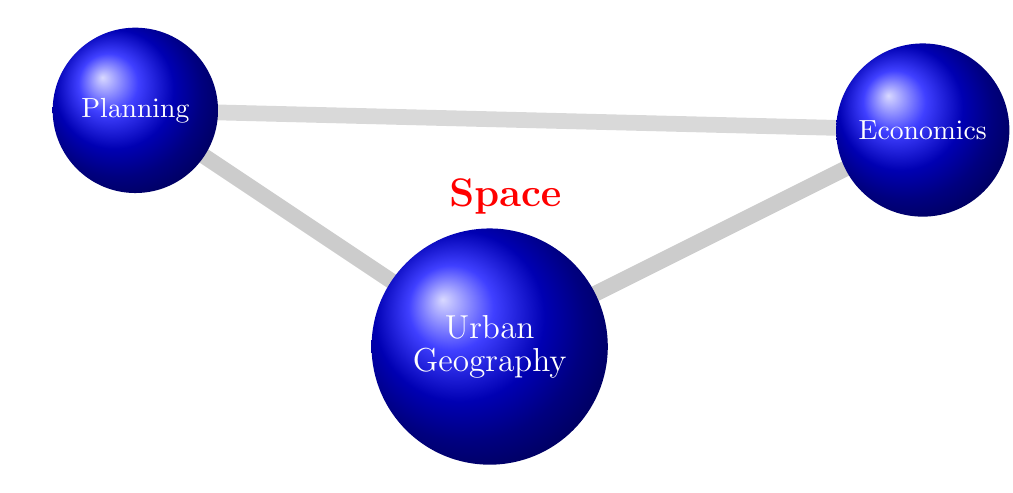
\begin{tikzpicture}{scale=.5}
% find color cotrol for ball. Tind way to stop line short of node
\coordinate (planning) at (-5,1);%PREFACE
\coordinate (economics) at (5,.75);%
 \coordinate (geography) at (-.5,-2); %history
\coordinate (finance) at (0,5); %

\draw [line width=2mm, black!15, ] (planning)--(economics);
\draw [line width=2mm, black!20, ] (geography)--(economics);
\draw [line width=2mm, black!20, ] (geography)--(planning);

%\draw [line width=2mm, black!25, ] (geography)--(finance);
%\draw [line width=2mm, black!20, ] (planning)--(finance);
%\draw [line width=2mm, black!20, ] (finance)--(economics);

\node [circle,shading=ball, minimum width=2.1   cm, white, align=center] (ball) at (planning) {Planning};
\node [circle,shading=ball, minimum width=2.2cm, white, align=center] (ball) at (economics) {Economics};
\node [circle,shading=ball, minimum width=3 . cm, white, align=center] (ball) at (geography)[text width=2cm] {\large Urban\\ Geography};

%\node [circle, shading=ball, minimum width=2.4cm, white, align=center] (ball) at (finance)[text width=2cm] {Finance};

\node at (-.3,-.1) [red] {\Large \textbf{Space}};
\end{tikzpicture}

Figure 1: The common concern of three fields
topic 

A simple economic insight -- that locational value gives rise to land rents -- provides an organizing principle for the three disciplines. Rent theory has a long history in economics, going back to thinkers such as Richard Cantillon (1680s-1734), François Quesnay (1694–1774), the marquis de Mirabeau (1715–1789) and Anne-Robert-Jacques Turgot (name physiocrat) and Adam Smith (1723-1790) and received its classic statement in Ricardo (1772-1823). Nearly contemporaneous thinker, Johann Heinrich  von Th\"unen (1783-1850) developed a planning model to guide the location of economic activities for an urban-agricultural society.  A version of that model  was reinvented in urban geography by XXX. Alonzo\footnote{We use a version of the well-established model of Alonso (1964), Muth (1969) and Mills (1967), and formalised by Wheaton (1974),}

We link the Alonzo model with more recent work on growth theory starting with Robert Solo's XXX and with the endogenous growth models of Lucas () and draw on Jane Jacobs's insight that endogenous urban growth  is. now driving economic development. Jacobs's insight is empirically supported by recent work in the complexity literature on urban scaling by XXXX ()




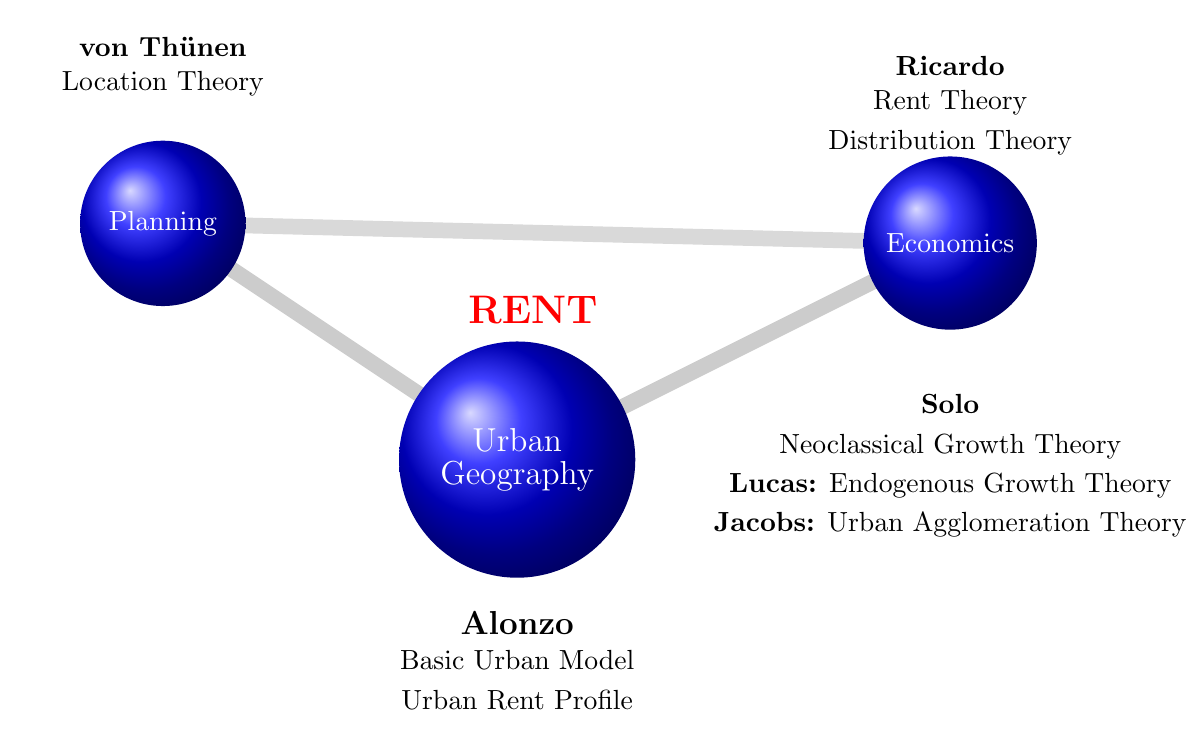
\begin{tikzpicture}{scale=.5}
% find color cotrol for ball. Tind way to stop line short of node
\coordinate (planning) at (-5,1);%PREFACE
\coordinate (economics) at (5,.75);%
 \coordinate (geography) at (-.5,-2); %history
\coordinate (finance) at (0,5); %

\draw [line width=2mm, black!15, ] (planning)--(economics);
\draw [line width=2mm, black!20, ] (geography)--(economics);
\draw [line width=2mm, black!20, ] (geography)--(planning);

%\draw [line width=2mm, black!25, ] (geography)--(finance);
%\draw [line width=2mm, black!20, ] (planning)--(finance);
%\draw [line width=2mm, black!20, ] (finance)--(economics);

\node [circle,shading=ball, minimum width=2.1   cm, white, align=center] (ball) at (planning) {Planning};
\node [circle,shading=ball, minimum width=2.2cm, white, align=center] (ball) at (economics) {Economics};
\node [circle,shading=ball, minimum width=3 . cm, white, align=center] (ball) at (geography)[text width=2cm] {\large Urban\\ Geography};

%\node [circle, shading=ball, minimum width=2.4cm, white, align=center] (ball) at (finance)[text width=2cm] {Finance};

\node at (-.3,-.1) [red] {\Large \textbf{RENT}};

% new stuff
\node at (planning) [above=2cm] {\textbf{von Th\"unen}};
\node at (planning) [above=1.5cm] {Location Theory};

\node at (economics) [above=2cm] {\textbf{Ricardo}};
\node at (economics) [above=1.5cm] {Rent Theory};
\node at (economics) [above=1.0cm] {Distribution Theory};

\node at (economics) [below=1.8cm] {\textbf{Solo}};
\node at (economics) [below=2.3cm] {Neoclassical Growth Theory};
\node at (economics) [below=2.8cm] {\textbf{Lucas:} Endogenous Growth Theory};
\node at (economics) [below=3.3cm] {\textbf{Jacobs:} Urban Agglomeration Theory};


\node at (geography) [below=1.8cm] {\textbf{\large Alonzo}};
\node at (geography) [below=2.3cm] {Basic Urban Model};
\node at (geography) [below=2.8cm] {Urban Rent Profile};
\end{tikzpicture}

Figure 3: space and value

Land rent was historically the basis of the wealth and political power of  the land-owning class in the era of the classical economists.


We further link the model of urban rents to emerging concerns about the financialization of the housing market. The key insight we offer is that the financialization  of the housing sector is a  form of rent-seeking that must have detrimental effects on urban development and on the well-being of urban residents.





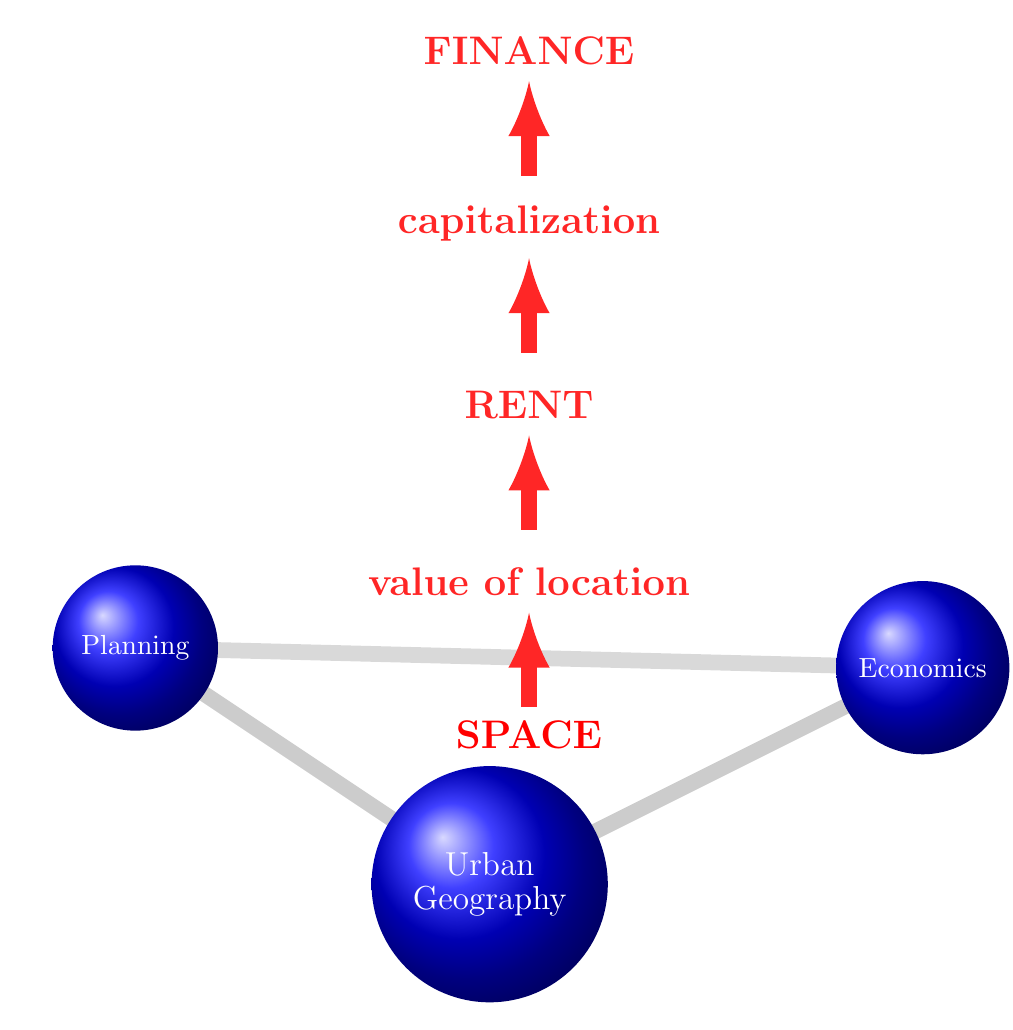
\begin{tikzpicture}{scale=.5}
% find color cotrol for ball. Tind way to stop line short of node
\coordinate (planning) at (-5,1);%PREFACE
\coordinate (economics) at (5,.75);%
 \coordinate (geography) at (-.5,-2); %history
\coordinate (finance) at (0,5); %

\draw [line width=2mm, black!15, ] (planning)--(economics);
\draw [line width=2mm, black!20, ] (geography)--(economics);
\draw [line width=2mm, black!20, ] (geography)--(planning);

%\draw [line width=2mm, black!25, ] (geography)--(finance);
%\draw [line width=2mm, black!20, ] (planning)--(finance);
%\draw [line width=2mm, black!20, ] (finance)--(economics);

\node [circle,shading=ball, minimum width=2.1   cm, white, align=center] (ball) at (planning) {Planning};
\node [circle,shading=ball, minimum width=2.2cm, white, align=center] (ball) at (economics) {Economics};
\node [circle,shading=ball, minimum width=3 . cm, white, align=center] (ball) at (geography)[text width=2cm] {\large Urban\\ Geography};

%\node [circle, shading=ball, minimum width=2.4cm, white, align=center] (ball) at (finance)[text width=2cm] {Finance};
\draw [line width=2mm, red!85, -latex ] (0, 7)--++(0,1.2)node[above=-.1] {\Large \textbf{FINANCE}};
\draw [line width=2mm, red!85, -latex ] (0, 4.75)--++(0,1.2)node[above=-.1] {\Large \textbf{capitalization}};
\draw [line width=2mm, red!85, -latex ] (0, 2.5)--++(0,1.2)node[above=-.1] {\Large \textbf{RENT}};
\draw [line width=2mm, red!85, -latex ] (0, .25)--++(0,1.2)node[above=-.1] {\Large \textbf{value of location}};
\node at (0,-.1) [red] {\Large \textbf{SPACE}};
\end{tikzpicture}



% \vspace {2cm}
% Figure 4 with finance

% \begin{tikzpicture}{scale=.5}
% % find color cotrol for ball. Tind way to stop line short of node
% \coordinate (planning) at (-5,1);%PREFACE
% \coordinate (economics) at (5,.75);%
%  \coordinate (geography) at (-.5,-2); %history
% \coordinate (finance) at (0,5); %

% \draw [line width=2mm, black!15, ] (planning)--(economics);
% \draw [line width=2mm, black!20, ] (geography)--(economics);
% \draw [line width=2mm, black!20, ] (geography)--(planning);

% \node at (-.3,2) [red] {\huge \textbf{RENT}};

% \draw [line width=3mm,  black!50,opacity=.5 ] (geography)--(finance);
% \draw [line width=2mm, black!20, ] (planning)--(finance);
% \draw [line width=2mm, black!20, ] (finance)--(economics);

% \node [circle,shading=ball, minimum width=2.1   cm, white, align=center] (ball) at (planning) {Planning};
% \node [circle,shading=ball, minimum width=2.2cm, white, align=center] (ball) at (economics) {Economics};
% \node [circle,shading=ball, minimum width=3 . cm, white, align=center] (ball) at (geography)[text width=2cm] {\large Urban\\ Geography};

% \node [circle, shading=ball, minimum width=2.4cm, white, align=center] (ball) at (finance)[text width=2cm] {Finance};


% \end{tikzpicture}

Summarizing the overall focus of the thesis,  we are concerned with the implication for urban development of growing rent extraction by the financial sector.  

\vspace {2cm}
Figure 4 with finance

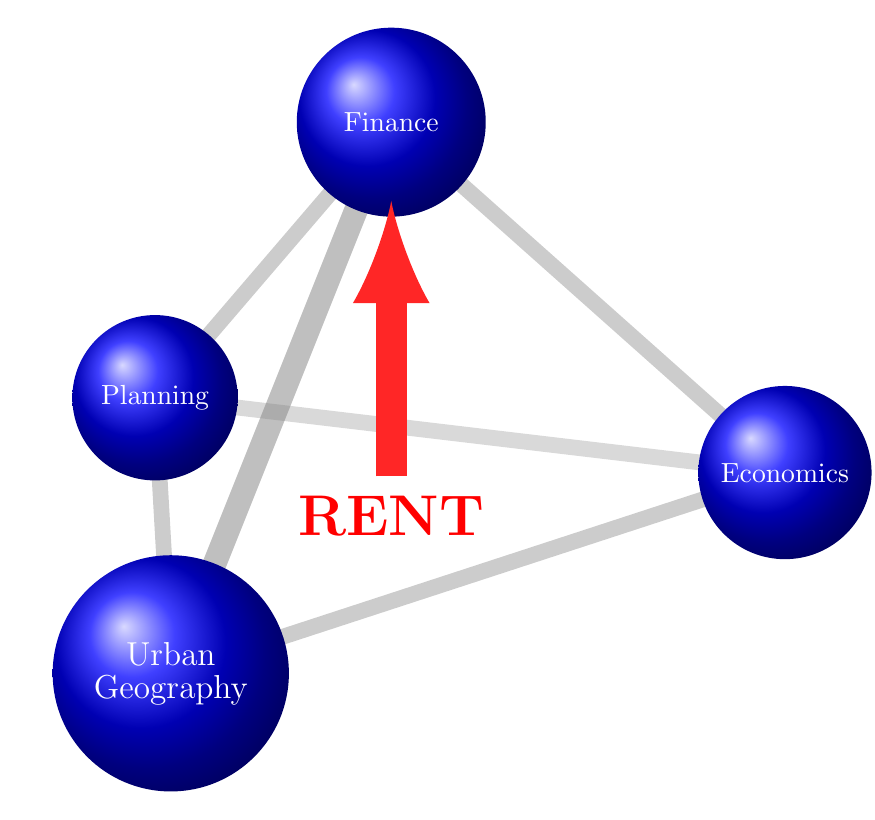
\begin{tikzpicture}{scale=.5}
% find color cotrol for ball. Tind way to stop line short of node
\coordinate (planning) at (-3,1.5);%PREFACE
\coordinate (economics) at (5,.55);%
 \coordinate (geography) at (-2.8,-2); %history
\coordinate (finance) at (0,5); %

\draw [line width=2mm, black!15, ] (planning)--(economics);
\draw [line width=2mm, black!20, ] (geography)--(economics);
\draw [line width=2mm, black!20, ] (geography)--(planning);

\node at (.0,0) [red] {\huge \textbf{RENT}};

\draw [line width=3mm,  black!50,opacity=.5 ] (geography)--(finance);
\draw [line width=2mm, black!20, ] (planning)--(finance);
\draw [line width=2mm, black!20, ] (finance)--(economics);

\node [circle,shading=ball, minimum width=2.1   cm, white, align=center] (ball) at (planning) {Planning};
\node [circle,shading=ball, minimum width=2.2cm, white, align=center] (ball) at (economics) {Economics};
\node [circle,shading=ball, minimum width=3 . cm, white, align=center] (ball) at (geography)[text width=2cm] {\large Urban\\ Geography};

\node [circle, shading=ball, minimum width=2.4cm, white, align=center] (ball) at (finance)[text width=2cm] {Finance};
\draw [line width=4mm, red!85, -latex ] (0, .5)--(0,4);


\end{tikzpicture}



\section{Document Overview}

\textbf{In chapter XXX}  we link classical rent theory, neoclassical production theory, neoclassical growth theory, the scaling literature, and urban spatial models.
To show how our model is directly connected with this broad collection of linked theories, we use the Cobb-Douglas function, which is used across this entire range of literature 

After we develop the mathematical description of the relationship among these will discuss  in more detail, rent theory and our contribution, scaling laws, ......  and other issues in the literature that draw on parts of this model and 

???  apply to the specific situation we're in why rent theory is related to discussions of exploitation why it might lead the inefficiencies, whether or not this links with other important models in the literature.

\textbf{In chapter XXX} we  provide a description of finacialization and show it is a a form of rent-seeking in the housing market and ?? the potential consequences of fiancialization in the housing market. 



\textbf{In chapter XXX} we  describe an illustrative agent-based model of the urban system. Most of the analysis of urban systems has employed analytical models with roots that go back to von Thunen () and more recently Alonzo. These models are extremely useful, but necessarily abstract from the concrete  and variable individual behaviour and  the details  of dynamics that make real cities path-dependent. XXX (Dawn) have shown that agent-based models can reproduce the features of the analytical models, at least in simple cases. 

ABMs can be run multiple times to produce distributions of expected outcomes, which makes them valuable in planning exercises. They also do not require  that we use a representative agent to make them tractable. Our model is intended to be elaborated  for such use. 

After we develop the mathematical description of the relationship among these will discuss in more detail, various relevant applications, and issues in the literature that draw on parts of this model and apply to the specific situation we're in why rent theory is related to discussions of exploitation why it might lead the inefficiencies, whether or not this links with other important models in the literature.


% Because we draw on a wide range of methods and literatures, we discuss the relevant literature and  methodologies in the chapters where they apply 



% \input{chapter-observations.tex}

% \part{A Model of Financialization and Rent}
% \chapter{Introduction}

Cities are a central feature of human society - Human beings are increasingly an urban species. Cities are one of the primary sources of technological development and increasing wealth. Behind these observations is a fundamental feature demonstrated in the recent literature on scaling laws: the productivity of cities increases super-linearly in population. Cities are the locus of a positive feedback loop: rising populations raises productivity, rising productivity attracts more people and resource.

Cities are where people live and work, where a great deal of production is concentrated, in addition to being where wealth is created and accumulated, cities are also where income is actually distributed. 

In Canada, there is a housing crisis. In the last few years, the need for affordable housing has come into focus as one of the most pressing issues facing Canadians. As more and more Canadians are finding housing unaffordable, the effects are being seen in everything from declining home ownership rates to an increasing number of Canadians unable to afford housing at all.

There has been extensive work on the drivers of the crisis, including supply shortages, stagnating incomes, and the finacialization of housing ownership.

There's been less work on the implications for productivity. The housing crisis raises the question of whether Canadian cities can continue to attract people and accumulate wealth for its residents and industries, whether in fact it can even sustain their growth.

This thesis presents a spatial model of the city that incorporates distributional issues and financialization and allows us to examine the productivity implications of the housing crisis. The model that incorporates the scaling of productivity in cities within a standard urban model. 
The urban model is based on those developed in geography, planning and urban economics. The organizing principle in  the spatial models of all three disciplines is an economic variable, land rent, which is the link to distribution, financialization and continuing productivity. *** (another sentence on why this is great)

The analysis makes clear that in addition to the recognized distributional consequences, the housing crisis has productivity impacts that should be considered in developing urban and housing policy. 


\subsection{OVERVIEW OF DOCUMENT}
\color{blue}

\textbf{In chapter XXX}  we link classical rent theory, neoclassical production theory, neoclassical growth theory, the scaling literature, and urban spatial models.
To show how our model is directly connected with this broad collection of linked theories, we use the Cobb-Douglas function, which is used across this entire range of literature 

After we develop the mathematical description of the relationship among these will discuss  in more detail, rent theory and our contribution, scaling laws, ......  and other issues in the literature that draw on parts of this model and 

???  apply to the specific situation we're in why rent theory is related to discussions of exploitation why it might lead the inefficiencies, whether or not this links with other important models in the literature.

\textbf{In chapter XXX} we  provide a description of finacialization and show it is a a form of rent-seeking in the housing market and ?? the potential consequences of fiancialization in the housing market. 



\textbf{In chapter XXX} we  describe an illustrative agent-based model of the urban system. Most of the analysis of urban systems has employed analytical models with roots that go back to von Thunen () and more recently Alonzo. These models are extremely useful, but necessarily abstract from the concrete  and variable individual behaviour and  the details  of dynamics that make real cities path-dependent. XXX (Dawn) have shown that agent-based models can reproduce the features of the analytical models, at least in simple cases. 

ABMs can be run multiple times to produce distributions of expected outcomes, which makes them valuable in planning exercises. They also do not require  that we use a representative agent to make them tractable. Our model is intended to be elaborated  for such use. 

After we develop the mathematical description of the relationship among these will discuss in more detail, various relevant applications, and issues in the literature that draw on parts of this model and apply to the specific situation we're in why rent theory is related to discussions of exploitation why it might lead the inefficiencies, whether or not this links with other important models in the literature.


\color{red}
Because we draw on a wide range of methods and literatures, we discuss the relevant literature and  nethodologies in the chapters where they apply 

\color{black}


Methodological questions: 

    - agent models (integrating theory more completely into agent models)
    
    - rent theory

Core model

    - static version
    
    - dynamic version

Simulations

Result---> hysterisis

policy

\subsubsection{OR (rougher):}

1. the core model and analysis - do a model of the endogenous dynamics of the model.

2. the resilience analysis -
but this is coupled with a larger system. we're interested in how it is coupled..

low interest rates have been key to financialization 
now they're going up?

we drive the system with signals to see how. and look at the external driving variables.

but what happens with changing interest rates? to explore we drive the system with external signal to explore how it is coupled with the larger economy and get an interesting resilience result, that it is actually a kind of ratchet pumping wealth out of communities on the upswing and on the downswing.

add interest, get a result which is hysteresis, which has policy implications
We get predictions about the implications of rising interest rates.

3.  policy analysis - finally we take a second step out to position the model within a larger dynamical system and do a systems analysis of the model and suggest policy implications. 

% \chapter{Antecedents of modern Urban Rent theory}
In this chapter, we link classical rent theory, neoclassical production theory, neoclassical growth theory, the scaling literature, and urban spatial models. 

%We use the Cobb-Douglas function %, which is used to cross this entire range of literature to illustrate each link and to show how our model is directly connected with this broad collection of linked theories. 
%The Cobb-Douglas function is a production function, expressing the output produced, in terms of inputs such as labour and capital.
%Our model connects to the results in this chapter at four points:



\section{Classical theories of production and distribution}
INTRODUCE RICARDO, CLASSICAL THEORIES - OR RESTRUCTURE AS AN INTRO SENTENCE.
MAYBE REVIEW SOME ALTERNATIVES/FRAME RICARDO
 % \subsection{Ricardo}

 The core social question that Ricardo addressed was who gets the surplus. % The question was pressing because it appeared that landlords were capturing the surplus without contributing to production while many of those who worked that land were very poor. 
Ricardo uses his model to explain the distribution of the product of the earth among the “three classes of the community” which is to say, to the owners of land, labour, and capital. 

% going back to the Physiocrates. 
% The physiocratic school of economics was the first to see labor as the sole source of value but, for the physiocrats, in the context of the prevalent European rural society of the time, only agricultural labor created a surplus. % actually? % detail for it was ag economy This was the theory? also the french enginneers- detail for start of math/calc-..
%The canonical reference for only agricultural labour mattering? For the definition of rent?

%Ricardo's famous 1815 discussion of capital and  land rent \footnote{ %\href{http://la.utexas.edu/users/hcleaver/368/368RicardoOnCornLaws.html}{An Essay on the Influence of a low Price of Corn on the Profits of Stock}; 
%showing the Inexpediency of Restrictions on Importation: With Remarks on Mr Malthus' Two Last Publications: "An Inquiry into the Nature and Progress of Rent," and "The Grounds of an Opinion on the Policy of restricting the Importation of Foreign Corn"} provides the canonical reference. 
% We haven't introduced this model or what kind of thing it is.
The concept of rent in economics must be distinguish from the common use of the term to mean the payment paid to rent a property. 

In the classical tradition, rent is the value landowners claimed for the use of their land. Ricardo defines rent strictly in this way, saying ``By rent I always mean the remuneration given to the landlord for the use of the original power of the land\footnote{'' David Ricardo corn laws note 7.}. % explan that ricardo used this as a formal definition of the term. he ....

For Ricardo, and for the classical economics in general however, land rent, is a kind of surplus value, that is an amount available after the costs of production have been paid, the term rent came to be used interchangeably with this more general concept in much of the classical work on rent.
%and the term rent has been used in a more general sense to other kinds of surplus value, as well as land rents 
as Saunders says in 1902, ``Of the concrete forms of income that have usually been classed as surplus, the rent of land was the earliest to be defined; and so prominent a position has been given to it that the terms "rent" and "surplus" have come to be used interchangeably.'' \footnote{Rent in Modern Economic Theory: An Essay in Distribution Author(s): Alvin Saunders Johnson, Publications of the American Economic Association, Nov., 1902, 3rd Series, Vol. 3, No. 4 (Nov., 1902), pp. 1-129}. 
So for instance professional sports players' income, above the opportunity cost they could get working at another position, is rent they capture for their skill. 

The classical idea of rent and rent can be illustrated with the story of a carter who picks up vegetables at the farm gate and transports them into town, where he sells them to a  storekeeper. %He pays the farmer at one end of the trip and is paid at the other. 
For simplicity, assume all farmers have the same cost of production, and the carters pay the farmer the farm gate price at the farm and receive the merchant price in town. 

\begin{figure}
    \begin{center}
     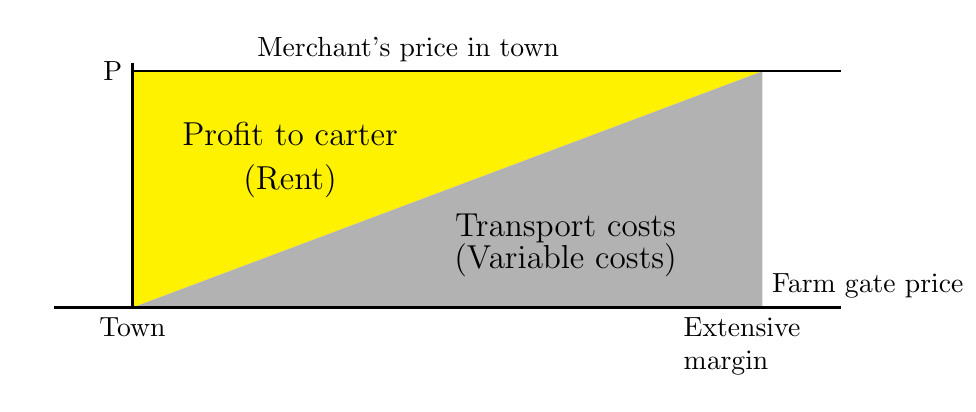
\begin{tikzpicture}[domain=0:2]
%\draw[thick,color=gray,step=.5cm, dashed] (-0.5,-.5) grid (3,3);
%\draw[line width=.01, green ] (0,0) -- (10,0) node[right  ] {Distance};
\node at (1,0) [below] {Town};
\fill[yellow]  (1,0) --(9,3)--(1,3) --cycle;
\fill[gray!60] (9,3) --(1,0)--(9,0) --cycle;

\draw[thick ] (1,3)node[left]{P}  -- (10,3);\node at (4.5,3)[above ] {Merchant's price in town} ;
\draw[thick ] (0,0)  -- (10,0); 

%\draw[thick,color=red] (1.5,0) -- (1.5,1) node[below right] {Fixed cost} -- (1.5,1.5) --(10,3.25)node[above left] {total cost};
\draw[thick] (1,0) -- (1,3.1) ;
\node[below,text width=2cm]at (9,0) {Extensive margin};
%\draw[ultra thick, blue,<-> ] (3,1.8) -- (3,2.5)node[left] {annual rent at a} -- (3,3) ; 
\node at (9,0)[above right] {Farm gate price};
\node  at (6.5,1){\large Transport costs};
\node  at (6.5,.6){\large (Variable costs)};
\node  at (3.,2.2){\large Profit to carter};
\node  at (3.,1.6){\large (Rent)};
\end{tikzpicture} 
    \caption{Transport costs, the yellow area, take a share of the profit for vegetables sold in the town}
    \label{fig:rent_ricardo}
    \end{center}
\end{figure}

In the figure \ref{fig:farm_rent}, total transport costs are shown as the yellow area. The area below the yellow triangle is profit for the carter. The carter makes a `profit' on the trip to the farm nearest to town, but there is a farm so far out  that transport costs eat up all the profit on the trip. That is as far as the carter will go\footnote{Note the similarity with Alonzo's urban model, illustrated in Fig \ref{Fig:rent_alonzo}.}. Ricardo termed this point the `extensive margin', the point at which there is no value for farming for the town. It is the limit for this use, and the profit there is zero. If the price goes up, the extensive margin moves out, and more land comes into production.

The land rent declines with distance from the town,\footnote{It also declines for less fertile land, where there is a higher cost of production.} At the extensive margin the land rent falls to zero. Even fertile land beyond the extensive margin will not be farmed because the product cannot be transported to market at a profit.\footnote{This simple example assumes that the land is uniformly productive and that there is only one product that can be marketed. Johann Heinrich von Th\"unen, in The Isolated state (Der isolierte Staat (1826)), provide a more complex analysis based on the same principles.} Transportation costs and the price of produce in town determine the size of the  rent triangle and therefore the amount of rent captured by the land-owning class.\footnote{The debate about the  `Corn Laws" that Ricardo  was engaged in was about whether Britain would allow wheat form Canada and Australia to enter, reducing the price of wheat and therefore reducing the income and influence of the land-owning class.} 

Together these two triangles/areas represent the ``produce of the earth'', but only the lower triangle is net income\footnote{ Termed the `\textit{produit net}' by the Physiocrats}. In modern supply and demand analysis it would be recognized as `producer surplus', the difference between what a producer gets for a good and what they would be willing to accept.

In Ricardo's case: the land owner delivers the grain to market and receives the merchant price. The profit is what the landowner could claim for the privilege of using the land %The profit now accrues to the landowner, and we call it land rent. For Ricardo, it was obvious that the land-owning class captured the land rent.
\footnote{In the modern economy, agricultural land rents may be captured by corporations,  either by owning the land or by controlling the supply chain.}  Landlord income is a locational land rent that exists because of the land's proximity to the market. 
 

%\subsection{A more explicit treatment}

Ricardo expounded a theory of land rent. While he did not write down a formal production function as later neoclassical theorists would, modern neoclassical production theory can be seen as having one of its origins in his work on classical economic theory.
In modern notation, Ricardo's model can be written:

\begin{equation} 
Y=F(K,L,N).
\label{Eqn:Prod1}
\end{equation} 

where $K$ is capital, $L$ is labour and $N$  is the natural resource  land.\footnote{This makes it a three factor model of production (cite us/lit) In principle any number of factors can be included.}  
Ricardo does not specify a functional form, but, %like mathematical neoclassical economists, 
he does assume diminishing returns to all factors. The landlord  receives the surplus generated by the land and the rest of the value of production goes to labour and to any capital employed in improving the land. 

The value of the land is the present discounted value of the surplus it generates, that is what it would be worth paying now, to capture the future rents from that land.


\subsection{Marx}


%Ricardo, agreeing with Malthus, essentially assumes that the wage is  just sufficient to reproduce the labouring class.\footnote{``In the natural advance of society, the wages of labour will have a tendency to fall, as far as they are regulated by supply and demand; for the supply of labourers will continue to increase at the same rate, while the demand for them will increase at a slower rate.''} He then explains the distribution of the fruits of labour on the land among the main classes of the economy.

 Marx shifted attention to the manufacturing economy in which the owners contributed the machinery, buildings, and even working capital to fund the workers until the product can be sold. %This contribution must be accumulated from their profits in the preceding cycle of production,  and has to be reinvested once the revenues of the current round have come in and the bills have been paid. Marx actually describes a circuit of capital from its form as money to its form as physical capital. 
As in Ricardo, however, labour is in surplus and capital is scarce. As in Ricardo the scarce factor owned by a special class - now the capitalists, is able to appropriate the is able to capture the surplus value. %Like Ricardo,  Marx saw the appropriation of surplus as without moral justification. 

Marx pointed to a new dynamic in capitalist systems - that productive capital is not fixed as land is, but  expands as surplus is reinvested. %He famously suggested that the expansion will eventually outrun the expansion of demand and the rate of return will fall, leaving capitalists unwilling to invest. % and creating a crisis. 

Marx gives the statement of the dynamic quality of the surplus
- work linking urban rents to the dynamic quality of the surplus in the urban system is in that tradition 
- how does the generative surplus gets distributed, its dynamics/the dynamics of the surplus. 
 
\subsection{Henry George} 


  Henry George, an influential American political economist,\footnote{Progress and Poverty: An Inquiry into the Cause of Industrial Depressions and of Increase of Want with Increase of Wealth: The Remedy (1879) book by social theorist and economist Henry George.}  returned to land rent with a new insight based on the emergence of the capitalist city: ``With the growth of population, land grows in value, and the men who work it must pay more for the privilege.'' For George the owners of urban land extract surplus in exactly the same way that owners of agricultural land in Ricardo's analysis. Where Marx saw the extravagant productivity of capital as the source of capitalist crises, George saw the extraction of wealth by land speculators as the mechanism that would bring on crises.
  
  Since land rent is not created by its owners, George argued that land rent should be seen as a social income - that it could be used to pay for all the needs of the community. The clearest statement of this view is found in Progress and Poverty: "We must make land common property." The same view was expressed by the Physiocrats who concluded  that ``ground rents'' should be the source of most or all taxes. They defined ground rent as that portion of all rent which is attributable only to the size and location of the parcel. George's analysis the `single tax' movement, which sought to shift all taxation to land  and resource rents.   
  
  In 1977, Joseph Stiglitz  showed, using a standard urban model, identified the conditions in which Henry George's "single tax" is  the only tax necessary to finance public expenditures.\footnote{Arnott, Richard J.; Joseph E. Stiglitz (November 1979). "Aggregate Land Rents, Expenditure on Public Goods, and Optimal City Size" (PDF). Quarterly Journal of Economics. 93 (4): 471–500. doi:10.2307/1884466. JSTOR 1884466. S2CID 53374401 }   The logic is fairly simple: if the public good increases productivity or the attractiveness of a city, attracting more people or businesses, land rents rise, and investment in the public good should proceed until the marginal cost of the public good is equal to the increase in land rent it brings. The result is now called the `Henry George theorem.'



The classical economists agreed that rents are unearned income. They did not emphasize, as George did, that land rents arise from labour's proximity to urban population and production.\footnote{To be fair, it was not lack of understanding, that the omission reveals, but rather lack of interest in explicitly examining urban land rent from residential or even industrial purposes.}% Ricardo von Thunen, Marx, Cantillon all grasped the notion of proximity to the market as part of the source land rent. The discussions seem to not gone farther than discussions of diffeerential and rents, however.  I just am not aware of them explicitly examining urban land rent for residential or even industrial purposes. 

%The need to be near a market or prodduction center is easily seen by considering a population at the carrying capacity of the land with individuals supporting themselves using purely local resources. There can be no land rent in this case. If a city rises that must be supplied from those still on the land, land close enough to the city will generate land rent. The value of the land is created by proximity to the city.



%  no separate and comprehensive data are provided on the amounts of land rents and subsoil rents charged and earned, because they are not officially regarded as part of value-added, and consequently are not included in the calculation of GDP (except for the value of productive lease contracts)     https://en.wikipedia.org/wiki/Differential_and_absolute_ground_rent#Rent_in_macro-economics    \href{https://en.wikipedia.org/wiki/Differential_and_absolute_ground_rent#Rent_in_macro-economics}{Wikipediat article on differential rent}

Stiglits is linking the capture of urban rents to productivity.

  \subsection{John Bates Clark and neoclassical distribution theory}
  Classical theories of distribution showed that ownership of a scarce and non-produced factor, land, was the  basis of rent extraction by the class of landowners. Profits were a bit puzzling in this context - Capital also earns its return from scarcity. Marshall pointed out, however, that scarcity profits (i.e., rent) would normally be competed away  as entrepreneurs entered the market in pursuit of those `excess' profits. He used the term `pseudo-rents' for these unearned but temporary incomes.\footnote{Alvin Saunders Johnson. Rent in Modern Economic Theory: An Essay in Distribution. AEA 3rd Series, Vol. 3, No. 4 (Nov., 1902), pp. 1-129 (129 pages)}

 John Bates Clark was one of the pioneers of marginalism and the neoclassical theory of  distribution.  The marginalist approach emphasized the rational decisions of economic agents in allocating their resources would lead them to allocate resources according to the value of the marginal product of the resource in production.  Initially a socialist like George, by 1986 he was praising the dynamical process of competition partly in opposition to the single tax movement George had initiated.  His (1891) ``Distribution as Determined by a Law of Rent,'' argued that, given  competition and homogeneous factors of production labor and capital, the division of the social product will be according to the productivity of the last (or marginal) physical input of units of labor and capital.\footnote{Responding to the "indictment that hangs over society" that it involves "exploiting labor," Clark wrote:

    It is the purpose of this work (his 1899 'Distribution of Wealth) to show that the distribution of the income of society is controlled by a natural law, and that this law, if it worked without friction, would give to every agent of production the amount of wealth which that agent creates. However wages may be adjusted by bargains freely made between individual men (i.e., without labor unions and other "market imperfections", the rates of pay that result from such transactions tend, it is here claimed, to equal that part of the product of industry which is traceable to the labor itself; and however interest (i.e., profit) may be adjusted by similarly free bargaining, it naturally tends to equal the fractional product that is separately traceable to capital.} 
 
Clark's analysis of income distribution does not contradict the classical view of rents, it simply displaces the analysis to the point where a competitive equilibrium prevails, and shifts attention away from the distribution of land rents. Rents are not earned by the marginal unit of land and  





\section{Neoclassical production theory}
The concept of a production function used by increasingly mathematical neoclassical economists and  rapidly developing statistical techniques  naturally led to attempts to identify the precise functional form that would describe the contributions of labour, capital, and income to output.
 
Mathematician Charles Cobb and Economist Paul Douglas came up with a specific and very convenient functional form\footnote{Cobb, C. W.; Douglas, P. H. (1928). "A Theory of Production"  American Economic Review. 18 (Supplement): 139–165. JSTOR 1811556. Retrieved 26 September 2016. The function had apparently previously been used by Knut Wicksell, Philip Wicksteed, and L\'eon Walras.} that captured much of what economists were talking about. The function is just a generalized arithmetic mean:
 
 \[Y=AK^\alpha L^\beta\]
 where $A$ is a constant scale factor, commonly called `Total Factor Productivity. This function becomes the workhorse of neoclassical growth theory in the second half  of the 20th century. Our urban model is a direct heir of those developments.

%The Cobb Douglas function has several convenient features. One is that the sum of the coefficents tells us the degree of returns to scale. If $\alpha+\beta = 1$, we have constant returns to scale,

%Another is that the coefficients of the factors, $\alpha$  and $\beta$ turn out to be the elasticities of output with respect to capital and labour respectively as well as the income share of the factor. These made it relatively easy for economists to combine national data on labour and capital stocks or income with output to test the model.

The Cobb–Douglas form was developed and almost immediately tested against statistical evidence in the USA by Cobb and Douglas between 1927–1947. It was  their widely circulated empirical work seems to have permanently associated this simple function with Cobb and Douglas for economists.

The Cobb-Douglas form captured  important regularities in the cross-sectional national data,\footnote{ A 2021 meta-analysis of 3186 estimates concluded that "the weight of evidence accumulated in the empirical literature emphatically rejects the Cobb-Douglas specification."Gechert, Havranek, Irsova, Kolcunova (2021), "Measuring capital-labor substitution: The importance of method choices and publication bias", Review of Economic Dynamics, doi:10.1016/j.red.2021.05.003, S2CID 236400765. More sophisticated models  such as the CES and translog functions have been developed  since.} 
but the estimates soon showed a systematic bias with time series. Essentially the value of the $A$ seemed to rise over time. Something that was not captured in the initial model  contributed to productivity over time: 
 \[Y=A(t)K^\alpha L^\beta\]



\section{MOVE SECTION BRINGING PRODUCTIVE LAND BACK IN Neoclassical production}

Ricardo analysis of land can be thourght of as:

\begin{equation} 
Y=F(K,L,N).
\label{Eqn:Prod1}
\end{equation} 
where $K$ is capital, $L$ is labour and $N$  is the natural resource  land.

Most modern neoclassical treatments of production have the same basic structure of the production function, but they simplify by omitting land: 

\begin{equation} 
Y=F(K,L).
\label{Eqn:Prod1}
\end{equation} 

    
Which makes sense for a number of reasons. The economy has shifted from agriculture to industry as well as
%Leaving land out of the model makes sense for a variety of reasons. 
And, according to the Ricardian theory, rent is a surplus above cost. It does not, therefore enter into price. Land is a fixed factor for society as a whole that is not consumed in  the process of production.  Furthermore, neoclassical treatments of production focus price determination based on the cost of the last unit used, the marginal  unit of input, while rents are generated on all of the inframarginal units, those units used earlier, which are more productive. The marginal unit of land generates no rents. In neoclassical analysis, the rents disappeared from view for this reason. This difference is at the heart of the distinction between classical and neoclassical economic theory. 

%John B. Davis. Ricardo's Theory of Profit and the Third Edition of the \textit{Principles}. Journal of the History of Economic Thought, 15, Spring 1993. °1993 by the History of Economic Society.
%``Questions arise, however, when one turns to exchange between a sector paying rent and one not.'' The Principles tells us that as cultivation is extended and exchange increases, profits fall while rents increase. 

Leaving land out, however, creates a problem in  the neoclassical growth theories we will examine below. Under the assumption of perfectly competitive goods and factors markets as well as marginal productivity pricing of capital and labor, neoclassical growth requires technical change to be generated outside the model because there are no resources left to innovate if both factors of production are paid their marginal product.\footnote{This follows from Euler’s theorem: if, for a given level of technology $\bar A$ output Y is produced according to a \textbf{constant returns to scale} and twice continuously differentiable function of capital and labor $F(K, L, \bar A)$, Euler’s theorem implies that $F_K K + F_L L=Y$, where $F_i$ is the marginal product of factor $i$. Payments to  capital and labor take up the entire national product and no resources are left to finance the production of technology-improving innovations. are paid their marginal product.} 
If, however, land is reintroduced, as it must be in an urban model, there must be rents and there is therefore as surplus available for innovation.
\footnote{An alternative and common approach is to assume imperfect competition, which may be based on increasing returns to scale, in which case firms with market power may achieve a surplus. ``Although seldom modeled outside the monopolistic competition framework, market incompleteness and imperfect competition are central to the new growth theories'' (Gilles Duranton, Growth and imperfect competition on factor markets: Increasing returns and distribution, European Economic Review, 44-2, 2000, 255-280), Similarly, Sjak Smulders and Theo van de Klundert conclude that ``Growth is higher in a more concentrated market provided that market power of firms is not too high,'' (Imperfect competition, concentration and growth with firm-specific R \& D, European Economic Review, 39-1, 1995,139-160).}
%I have not followed this track down to give references.

% ALSO Imperfect Competition and Total Factor Productivity Growth  AZZEDDINE M. AZZAM, ELENA LOPEZ and RIGOBERTO A. LOPEZ. Journal of Productivity Analysis. Vol. 22, No. 3 (November, 2004), pp. 173-184 (12 pages)

%Sjak Smulders and Theo van de Klundert.Imperfect competition, concentration and growth with firm-specific R & D European Economic Review. Volume 39, Issue 1, January 1995, Pages 139-160
% Duranton, Gilles (1997) Essays on growth: imperfect competition, labour supply and local public goods. PhD thesis, London School of Economics and Political Science.  http://etheses.lse.ac.uk/1471/1/U105715.pdf

%Alberto Bucci.  R&D, Imperfect Competition and Growth with Human Capital Accumulation, 2003. Scottish Journal of Political Economy. https://doi.org/10.1111/1467-9485.5004004. This paper studies the long-run consequences of imperfect competition on growth and the sectoral distribution of skills within an R&D-based growth model with human capital accumulation. We find that steady-state growth is driven only by incentives to accumulate skills. In the model imperfect competition has a positive growth effect, while influencing the allocation of human capital to the different economic activities employing this factor input. Contrary to general wisdom, the share of resources invested in R&D turns out not to be monotonically increasing in the product market power and its correlation with the equilibrium output growth rate is not unambiguous.

%NOTE URBAN COMPETITION PROVIDES INCENTIVES TO UPGRADE SKILLS!!!


% Both the Solow (1956) growth model and its Ramsey–Cass–Koopmans counterpart featuring an endogenous saving rate (Ramsey, 1928; Cass, 1965; Koopmans, 1965) see technical change as purely exogenous. In fact, under the assumption of perfectly competitive goods and factors markets as well as marginal productivity pricing of capital and labor, neoclassical growth requires technical change to be generated outside the model because there are no resources left to innovate if both factors of production. 

%  This follows from Euler’s theorem: if, for a given level of technology $\bar A$ output Y is produced according to a constant returns to scale and twice continuously differentiable function of capital and labor $F(K, L, \bar A)$, Euler’s theorem implies that $F_K K + F_L L=Y$, where $F_i$ is the marginal product of factor $i$. Hence, remunerating capital and labor takes up the entire national product, and no resources are left to finance the production of technology-improving innovations. Accordingly, the growth rate of technology will $\frac{\dot{A}}{A}=g_A$ is necessarily exogenous. %Focusing on balanced growth and 
% assuming that technical progress is labor augmenting (Uzawa, 1961), we can rewrite the production function as $F(K, AL$), where $AL$ is a measure of labor in efficiency units, or effective workers. Let k = K/(AL). Then, output per effective worker is y =Y/(AL)=f (k). Population grows at the constant rate n > 0 and, as we will assume throughout the whole paper, capital does not depreciate. The steady state of the Solow model solves

% $\frac{f(k_{ss}}{k_{ss}} = \frac{n+g_A}{s}kss s$

% Journal of Economic Surveys (2017) Vol. 31, No. 5, pp. 1272–1303 \c ECONOMIC THEORIES 1275


Classical rent re-appears in neoclassical theory as `economic rent' (``a money payment made for a factor of production that is over and above the minimum payment to keep it in its present use,'')  as quasi-or pseudo-rents (non-equilibrium rents that will be competed away in a competitive equilibrium according to Marshall.\footnote{see Lewis Cecil 4 Rent Under the Assumption of Exhaustibility, Quarterly Journal of Economics, May, 1914, Vol. 28, No. 3 (May, 1914), pp. 466-489}),  as consumer  and producer surplus in supply and demand analysis,  as rent profiles or Pseudo-rent curves in urban theory, as a major concern on resource economics, and the theory of rent-seeking. Economic rent is a surplus insofar as its payment is not necessary to ensure a supply of a particular factor of production. 


% HOUSING RENT IN THE NATIONAL ACCOUNTS
%   Owner-occupied housing is included in Peersonal Consumption Expenditure because the National Income and Producgt Accounts (NIPAs) treat the owner-occupant as if it were a rental business, or in other words, a landlord renting to him or herself. That is, BEA imputes a value for the services of owner-occupied housing (space rent) based on the rents charged for similar tenant-occupied housing, and this value is included in GDP as part of personal consumption expenditures. This imputation is necessary in order for GDP to be invariant when housing units shift between tenant occupancy and owner occupancy.


%Ricardo  clearly understood and used the concept of diminishing marginal product. This shows in his use of the terms ``extensive margin'' and ``intensive margin'' to explain the income of the landowner. He focussed on the difference between the cost of production on a unit of land and the revenue generated. The landlord would rent out all the land which generated at least enough to pay all the costs. Anything in excess of the costs could be charged as land rent to a tenant farmer.



%Clearly in his model there are two basic productive factors, land and labour. The landlord  receives the surplus generated by the land and the rest of the value of production goes to labour. 
Recent urban models, on the other hand, tend to ignore the production process and consider the locational implications of land and transportation costs location of people. Wealth distribution is often ignored. 


  \section{Neoclassical growth theories}  

 \subsection{The Solow-Swann growth model}
In 1956 Robert Solow\footnote{A Contribution to the Theory of Economic Growth,  Robert M. Solow, The Quarterly Journal of Economics, Vol. 70, No. 1 (Feb., 1956), pp. 65-94. Stable URL: http://www.jstor.org/stable/1884513} provided a possible explanation, opening the field for a further series of refinements in an enterprise that became known as ``growth theory.''
\footnote{Solow and his contemporary, Edward F. Denison in his 1961 monograph, \textit{The Sources of Economic Growth in the United States}, were attempting to account for the main features of U.S. economic growth, not to provide a theory of economic development.}%   R.E. Lucas, Jr., On the mechanics of economic development.}

Solow argued ``As a result of exogenous population growth the labor force increases at a constant relative rate n,'' so
  \[L(t)= L_0e^{nt}\] 
If we insert this term into the production function 
 \begin{eqnarray}
 Y&=cK^\alpha (L_0e^{nt})^\beta\\
    &=c(e^{nt})^{\beta}K^\alpha L^\beta\\
  %  &=A(t)K^\alpha L^{1-\alpha} \label{Eq:Solow}
 \end{eqnarray}
we see that $A$ becomes
 \[A(t)=c(e^{nt})^\beta\]
and we have a version of the time-dependent term needed to  allow the model to track the data better. More than half  of the cross-country variation in income can be explained by per capita saving and population growth alone.



%???       It is no surprise that adding a variable allowed the model to track the data better. More  interesting is that the appearance of term $1-\alpha}$ in the scale factor $A$ suggests a spillover effect of human capital on the productivity of other factors.\footnote{Breton, T. R. (2013). "Were Mankiw, Romer, and Weil Right? A Reconciliation of the Micro and Macro Effects of Schooling on Income" (PDF). Macroeconomic Dynamics. 17 (5): 1023–1054. doi:10.1017/S1365100511000824. hdl:10784/578. S2CID 154355849.}  

%The estimated model explained 78\% of the variation in income across countries.
% the estimates of $\beta$ implied that\textbf{ human capital's external effects on national income are greater than its direct effect on workers' salaries.}%(\url{https://en.wikipedia.org/wiki/Solow\%E2\%80\%93Swan_model)}.  Theodore Breton provided an insight that reconciled the large effect of human capital from schooling in the Mankiw, Romer, and Weil model with the smaller effect of schooling on workers' salaries. He demonstrated that the mathematical properties of the model include significant external effects between the factors of production because human capital and physical capital are multiplicative factors of production.[20] The external effect of human capital on the productivity of physical capital is evident in the marginal product of physical capital:
%    \[ MPK={\frac {\partial Y}{\partial K}}=\frac {\alpha A^{1-\alpha }(H/L)^{\beta }}{(K/L)^{1-\alpha} }\]


Solow's 1956 paper stimulated a vast literature in the 1960s, exploring many variations on the original one-sector structure. % (per Lucas on mechanics), See Burmeister and Dobell (1970) for an excellent introduction and survey. 
In these models, saving and population growth rates determine the growth trend of the economy. An important  contribution of the neoclassical framework stems from its ability to quantify the effects of various influences on growth. The estimated influences of saving and population growth with the Solow model appear too large, however.%Ludcas on the mechanics of ec dev
\footnote{In 1992, N. Gregory Mankiw, David Romer %(not to be confused with Paul M. Romer, mentioned above and below) 
and David N. Weil analyzed Solow’s Model in their paper “Contribution to the Empirics of Economic Growth” and  showed that %Solow correctly predicts the directions of saving and population growth, but not the orders of magnitude. Furthermore they pointed out that, 
if the model was augmented by including human capital $H$, it would fit the data even better.   (Mankiw et al. 1992). Their equation was, in our notation   \[Y=A(t)K^\alpha H^\gamma L^\beta\label{Eq:Mankiw}\] They assume $\alpha+\gamma<1$ which implies decreasing returns to all capital.}

To understand the relation between saving, population growth, and income, it was necessary to go beyond the textbook Solow model, which assumed  diminishing returns to capital and labor separately and constant returns to both factors jointly,


 MISSED Mankiw et al equation 
 % The  model became\footnote{Because they work with time series, all the quantities are dated. We omit the time marker for notational simplicity.}

In 1988, Robert E. Lucas would observe that ``It seems to be universally agreed that the model ... is not a theory of economic development.   \dots while it is not exactly wrong to describe these differences (in GDP  growth rates) by an exogenous, exponential term like A(t) neither is it useful to do so. We want a formalism that leads us to think about individual decisions to acquire knowledge, and about the consequences of these decisions for productivity.''\footnote{Lucas,  Robert E. On the Mechanics of Economic Development. Journal of Monetary Economics 22, 1988 3-42} 

% NOTE for  K   
%If we replace the labor-capital technology of the Solow model with a land-labor technology of the same form, and treat labor as the mobile factor and land as the immobile, we obtain a model that predicts exactly the immigration flows that occurred and for exactly the reason - factor price differentials - that motivated these historical flows



One of the predictions of the neoclassical growth model, even  when the concept of capital includes human capital, is that without  continuing improvements in technology, per capita income growth eventually ceases on the equilibrium path. 
By treating technological change as exogenous, neoclassical growth theory could not focus on the fundamental forces which determine long-run growth of nations. Theorists got around the problem to some extent by assuming that technological progress occurs in an exogenous manner. 

The models that followed, starting with Arrow's 1962 model of `learning by doing', introduce human capital and learning in a variety of ways. This is a central insight. Human capital may enter  as a stock that accumulates in the firm or the sector (Arrow (1962), Levhari (1966), and Sheshinski (1967b)) (proxied by aggregate prior capital investment.)
%(Levhari-Sheshinski)as  the experience of workers, the number of units previously produced, 
or the amount of innovation in other firms and sectors. % ( King and Robson )


Identifying  plausible ways that human capital might affect development was relatively easy. Measurement of human capital presents great practical difficulties. To extract the implications of a particular path, it was also necessary to construct a tractable model, analyze its dynamic properties, and find proxy data to test the initial hypothesis.   A series of papers did exactly that.

Kenneth Arrow (1962) gave a dynamic interpretation to increasing returns by emphasizing 'Learning by Doing'. This was an early attempt to render technological progress endogenous in growth models by making the productivity of a given firm an increasing function of cumulative aggregate investment for the industry. Productivity rises with cumulative firm output.


 It is important to note that these models all open the possibility that governments can  promote growth through investment in education, research, technology transfer, and incentives for firms.

\subsection{Endogenous (neoclassical) Growth Models}
A new wave of research on economic growth was stimulated by Romer (1986) and Lucas (1988). In their models, returns to scale are external to single economic agents and internal to a sector or larger parts of the economy. We apply the same insight to urban models to incorporate the growth-enhancing effect of agglomeration. 

%Basically, two branches have developed, pioneered by Romer (1990) and Lucas (1988). CHECK THESE SOURCES

Paul Romer's 1986  model\footnote{ based on his 1983 thesis} describes `learning by investment'. In this model, the increase in total factor productivity depends on firms’ learning, or investment in knowledge accumulation through research, rather than output. He models the incentives for the production of knowledge explicitly. The production function  can be written

\[Y = A(R^T)R^\gamma  K^\alpha L^\beta) \]
Where $R(\equiv R_i)$ is the research effort of the specific firm, and $R^T=\sum_iR_i$ is the total research in the industry,  $R$ is a choice variable for the firm, which is to say, it decides how much to invest in research. 

A notable feature of this model is the spillover effect on all other firms of the firm's investment through the Total Factor Productivity term,  $A(R^T)$. \textbf{This is the logic of our own model of agglomeration effects in the city.}



In 1988 Lucas also argued that technical progress is not exogenous, but endogenous. He proposed a model that is very close technically to the similar models of Arrow (1962), Uzawa (1965)and Romer (1986). Following our notation, 
\[ Y = A(H^e) K^\alpha (HeL)^\beta \] 
where $H^e$ is the economy's average level of skill (human capital).  Improvements in skill in any firm  increase overall productivity.  $HeL$  can be understood as the `effective' labour force of the firm. It is a product of $L$, size of the workforce. $H$, is the skill level of the firm's workers, and $e$, is the fraction of work time spent working. $1-e$ is the fraction of worker time  spent in training. The  special feature is that $e$ is a choice variable for the firm.\footnote{It could as easily be a choice variable for workers in the aggregate model.} More time training increase $H$ but reduces $e$, so the firm faces a tradeoff.


The difference between Romer and Lucas style theories is that endogenous growth in the theory of Romer is caused by accumulating technology (or knowledge), while in Lucas it is through training (accumulating human capital)\footnote{Although it is not of direct concern for our work, it is useful to recognize that much of the emphasis in these models is on finding the conditions that can explain the observed long term  and growth over and above that driven by exogenous population or technology growth. }

%THIS NEXT PARAGRAPH A SIMPLE COPY. FIND SOURCE

Again we see the  internal effects of human capital, where the individual worker undergoing training becomes more productive, and an external or `spillover' effect which increases the productivity of the economy. 
The evidence supports the existence of significant learning spillovers in a variety of industries. Using survey data, Mansfield (1985) found that information about new processes and products in ten industries surveyed had widely diffused within a year. Spillovers have also been found in econometric studies: Irwin and Klenow (1994) find them in semiconductors; Thornton and Thompson (2001) in wartime shipbuilding; Lieberman (1989) in chemicals; Foster and Rosenzweig (1995) in the adoption of high-yielding seed varieties; and Conley and Udry (2007) in the adoption of best practices by Ghanaian pineapple farmers. 

\textbf{ NOTE for Kirsten:  Neoclassical  growth theory predicts that growth rates of different countries with same rates of saving and population growth and with access to the same technology will converge. In  endogenous growth theory there is no force leading to the convergence of growth rates of different countries with closed economies. If the logic extends to urban systems as we believe it does, growth rates of cities will also diverge.}

\subsection{Neoclassical Production Theory and the City}
%\href{https://www.yourarticlelibrary.com/economics/new-theory-of-growth-of-economic-development/38329}{New Theory of Growth of Economic Development}Supriya Guru

In all of these models, the unit of analysis is the nation,  or the firm. Lucas has suggested,\footnote{Journal of Monetary Economics 22 (1988) 3-42.  ON THE MECHANICS OF ECONOMIC DEVELOPMENT*
Robert E. LUCAS, Jr., University of Chicago, Chicago, 1L 60637, USA}
however, that `` a national economy is a completely arbitrary unit to consider.'' and that ``we know from ordinary experience that there are group interactions that are central to individual productivity and that involve groups larger than the immediate family and smaller than the human race as a whole.''  


As a result, ``following very closely the lead of Jane Jacobs, whose remarkable book The Economy of Cities (1969)'', Lucas goes on to suggest `` that the 'force' we need to postulate account for the central role of cities in economic life is of exactly the same character as the 'external human capital' I have postulated as a force to account for certain features of aggregative development.''  He concludes that if this is so, ``\textbf{\dots land rents should provide an indirect measure of this force (emphasis  ours)}, in much the same way that schooling-induced earnings differentials provide a measure of the productive effects of internal human capital. ''

This insight, which parallels ours, has not been adequately explored, in our view.  Allowing Lucas to expand on his observation, 


\begin{quotation}
    Her emphasis on the role of cities in economic growth stems from the observation that a city, economically, is like the nucleus of an atom: If we postulate only the usual list of economic forces, cities should fly apart. \textbf{The theory of production contains nothing to hold a city together.} (empahsis ours) A city is simply a collection of factors of production - capital, people, and land - and land is always far cheaper outside cities than inside. Why don't capital and people move outside, combining themselves with cheaper land and thereby increasing profits? Of course, people like to live near shopping and shops need to be located near their customers, but circular considerations of this kind explain only shopping centers, not cities. Cities are centered on wholesale trade and primary producers, and a theory that accounts for their existence has to explain why these producers are apparently choosing high rather than low-cost modes of operation.
\end{quotation}

This observation provides a natural link to the scaling literature on cities.


\section{Cities and the Scaling Literature}
Neoclassical production theory does not address the spatial structure of the economy. Why are there cities? What drives the historic transition from land-based agricultural society to a much denser urban society? 

In The Economy of Cities (1969) Jane Jacobs argued that when people come together in cities they make each other more productive. This is in essence, a theory of urban agglomeration that could be written
\begin{equation}\label{eq:LtoN}
Y = A(t) K(t)^\alpha L^\beta 
\end{equation}
where $L$ stands for the size of the urban labour force. Since urban labour force and population are closely correlated, the familiar model is  observationally equivalent to
\begin{equation}\label{eq:N2}
Y = A(t)N^{\alpha+\beta}
\end{equation}
\footnote{ To see why, let  $cN$ be labour employed by capital in firms, where $N$ represents the urban population and  assume a constant capital-labor ratio $1/d$. Replace $K$ with $dcN$
\[Y = A(t) (dcN)^\alpha (cN)^\beta) \]
But  $dc^\alpha$ and $c^\beta$  are simply  multiplicative constants that can be incorporated into the scale factor $A$, so  the function becomes 
\[Y = A(d, c,\alpha, \beta, t)N^{\alpha+\beta}\]
}

A model of a national economy that uses the number of urban dwellers would track as well using the number employed. As countries develop, cities account for an ever-increasing share of  national populations and an ever-increasing share of national income.  This is  even more likely when we recall that the principle insights coming out of neoclassical growth theory point to human capital and education as the mystery factor in growth and cities are where the most skilled workers concentrate and where the strongest educational institutions tend to be. The mysterious contribution to growth pursued in the previous sections might  actually be a consequence of urbanization.

We have conventional diminishing returns to scale  if we impose the standard neoclassical assumption, 
$\alpha +\beta <1 $.\footnote{
The required condition is that 
$Y(\delta K,\delta L< \delta Y(K,L)$. 
In the function that we use to illustrate the models, 
$Y(\delta K,\delta L)= \delta^{\alpha +\beta}Y < Y(K,L)$.} 
That leaves us with a question: what do we need for Equation~\ref{eq:N1} to represent Jacobs' observation?  

The answer lies in making the synergies that Jacobs point to explicit: we require $N$ to generate a spillover effect similar to those  identified in neoclassical growth theory. There are three obvious generic ways to introduce such a term: $N$ can augment $A$, $K$, or $L$, 

NEEDS ALIGNMENT
  
\[Y = A*N^\gamma K^\alpha N^\beta= AK^\alpha N^{\beta+\gamma}\]
\[Y = A (N^\gamma* K)^\alpha  N^\beta= AK^\alpha N^{\beta+\gamma^\alpha}\]
\[Y = A K^\alpha (N^\gamma* N)^\beta= AK^\alpha N^{\beta+\gamma}\]

Each of these yields a form of
\[Y = AN^\psi\]
where $\psi> \alpha +\beta$ and may be greater than one. 
The question now is whether we can find estimates of $\psi$.

The evidence we need comes from another field. Complex systems theory is concerned with identifying and characterizing common design elements that are observed across diverse natural, technological and social complex systems. It focuses on general principles  identified in complex systems across many fields such as biology, physiology, ecology, stock markets, multi-user online  networks, data systems, human settlements.and urban systems.

Scaling analysis is a tool developed in complex systems science to investigate how extensive properties of the system vary with a system's size.  or scale.  In urban science, there are now many studies of  the relationships between urban population size and  features like urban economic output,  area, growth, traffic congestion costs, and even social  indicators like crime and homicide rates. Our particular interest is in studies linking city population  and  economic output. 

The model used is familiar. Omitting subscripts for time, $t$ and city, $i$, \footnote{Bettancourt (2021) writes the model \[Y_i = Y_0(t)N_i(t)^\beta e^{\xi(t)}\]. }
\[Y = Y_0e^{n(t)}N^\beta\]
where $Y_0$ is an initial value. Notice that this looks exactly like the form that we saw in the 
Solow-Swan model with the transform from $K^\alpha L^\beta$ to $N$.  The interpretation is different because the model is used to estimate the parameter $\beta$ and $e^{n(t)}$ is described  as an error term of the form commonly used in estimating multiplicative time-series models. As a result estimates of $\beta$  can be used as estimates  of $\psi$.

\vspace{1cm}
\textbf{\Large COPY BOTTOM FIVE ROWS OF TABLE ON BETTANCOURT PAGE 67}  


\vspace{2cm}
The empirical scale factor is a feature of  a static urban system, but, as we have seen it is essentially a growth model. If the population rises, output must rise more than proportionately, but if the population responds to the share of output, the population should then rise. This is a 

Much of growth theory was concerned with identifying the dynamics of such systems and in particular with the implications for the growth of incomes. The growth models, however, were not spatial models, and therefore abstracted from land rents And distribution. They have nothing to say about the distribution of city product and the effect that distribution might have on growth.\footnote{Early models employ a macroeconomic savings function which usually has a fixed savings rate, with savings being reinvested in productive capital. } 

\vspace{2cm}


\section{Does this belong here? Model stages}

Our model has three stages: first, a production function, modeling how urban regions generate wealth,  second a spatial model of an urban housing market, and third, an analysis of distribution within that model 

In this section, we introduce the basic structure of the production side and connect it to the literature on urban scaling. The basic scaling result at the level of the city allows us to incorporate the effect of agglomeration in a standard  circular-city model in a simple way, avoiding the need to explicitly model labour markets and firms.\footnote{Explicitly modeling labour markets and firms is a natural way to specify the model more completely, but it would require introducing many ancillary assumptions and selecting among alternative models of agglomeration, when when we want to focus on distributional and growth-affecting features of the system.}

\begin{enumerate}
    \item to introduce  the productive nature of cities we basically assume the presence of scaling. Given  that the scaling literature gives us an estimate of the economies of scale in a production function this allows us to simplify the model and focus on the features of the urban system rather than on fully specifying a production system. In our model, the city  exhibits economies of scale with respect to population directly. 

     \item  productivity of the city to generates an economic value for land that gives rise to rents

    \item  the rental value of land structures the spatial structure of the city

    \item we exploit the rent model and transport costs to get  distributional consequences
\end{enumerate}

\section{Equilibrium city size  in terms of scale factor} 
At this point we can briefly describe how the discussion of this chapter relates to our overall modelling. There are four basic equations in the model. The first two link output and the wage to population. 






\subsubsection{population and output}
Equation one, following Bettencourt (p65) says that  urban productivity is proportional to population via a scale factor: 
\[Y\propto N^{\beta}\]  
\footnote{ In contemporary US cities productivity increases by about 11\% with each doubling of their population.  Urban Scaling and the Production Function for Cities Lobo J, Bettencourt LMA, Strumsky D, West GB (2013) PLOS ONE 8(3): e58407. https://doi.org/10.1371/journal.pone.0058407 },
and has both theoretical and empirical support. 

% \begin{tabular}{ll}
% $Y$ is &Aggregate urban output, or GDP \\
% %$\alpha$ & agricultural wage\\
% $G$ is&a `prefactor', possibly time dependent, an initial population\\
%  $N$ is& city population\\
% $ \beta$  is& scale factor, the elasticity of output with respect to city population .\\
% \end{tabular}\vspace{.5cm}

This is illustrated below for $\beta=1.13$.



\begin{figure}
    \begin{center}
    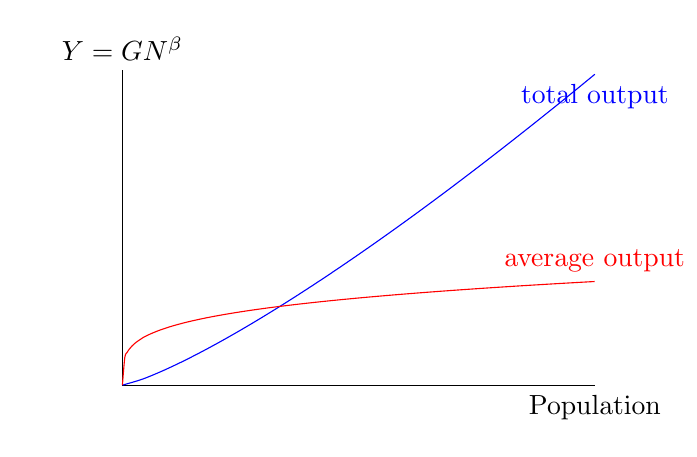
\begin{tikzpicture}
      \draw (0,4)node[above]{$Y= GN^{\beta}$}--(0,0) --(6,0)node[below]{Population};
       \draw[scale=1, domain=0:6, smooth, variable=\x, blue] plot ({\x}, {(\x/2)^1.25})node[below]{total output };% divide by 2 to get it on the plot
       %\draw (0,1)node[left]{$\alpha$}--(6,3.5)node[left]{$\alpha +\rho P$};
      \draw[scale=1, samples=200,domain=0:6, smooth, variable=\x, red] plot ({\x}, {(\x/2)^.25})node[above]{average output};% THis is the wage plot
           %   \draw[red] plot[samples=200, domain=-0:6] function {(\x/2)^.25};%node[above]{wage};
      %  \node [left] at (0,2){$w=\rho P$};
         % \draw [dashed](0,3)node[left]{$Y_i$}--(6,3);
    \end{tikzpicture}\vspace{.5cm}
    \caption{Urban productivity is proportional to population, $\beta=1.13$}
    \label{fig:scale_output}
    \end{center}
\end{figure}
 
 This figure illustrates a worry for me - the \textbf{average income} - {a proxy for the wage?) rises with $N$ but not more rapidly than transportation costs.
 
\subsubsection{Output and wage}
We need a combination of classical and neoclassical distribution theory.

City output is divided among the classes of society. Neoclassical theory suggests wages are allocated according to marginal product and classical theory suggests rents according to the pattern of ownership.

Equation one, in effect determines a wage, (Given the observed values for the scaling coefficients for total wages and labor, $bW < 1.15$ and $bL < 1$, )  although there are many possible distributional specifications and many possible labour market and firm structures. Bettencourt provides two  estimates,  1.11 and 1.35, for the scale factor for urban personal income in the Brazil and South Africa respectively.\footnote{A more recent  study supports the Bettancourt results for Chiin Wu W, Zhao H, Tan Q, Gao P. An Urban Scaling Estimation Method in a Heterogeneity Variance Perspective. Entropy (Basel). 2019 Mar 28;21(4):337. doi: 10.3390/e21040337. PMID: 33267051; PMCID: PMC7514821.} 

\subsubsection{Wage and city size}
The third determines the extent of the city. This comes form the Alonzo model discussed in chapter XXXXA. 

\begin{figure}
    \begin{center}
     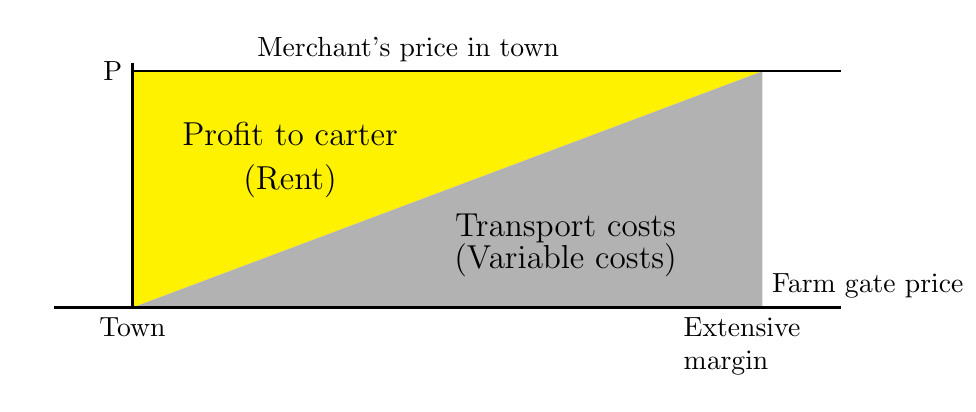
\begin{tikzpicture}[domain=0:2]
%\draw[thick,color=gray,step=.5cm, dashed] (-0.5,-.5) grid (3,3);
%\draw[line width=.01, green ] (0,0) -- (10,0) node[right  ] {Distance};
\node at (1,0) [below] {Town};
\fill[yellow]  (1,0) --(9,3)--(1,3) --cycle;
\fill[gray!60] (9,3) --(1,0)--(9,0) --cycle;

\draw[thick ] (1,3)node[left]{P}  -- (10,3);\node at (4.5,3)[above ] {Merchant's price in town} ;
\draw[thick ] (0,0)  -- (10,0); 

%\draw[thick,color=red] (1.5,0) -- (1.5,1) node[below right] {Fixed cost} -- (1.5,1.5) --(10,3.25)node[above left] {total cost};
\draw[thick] (1,0) -- (1,3.1) ;
\node[below,text width=2cm]at (9,0) {Extensive margin};
%\draw[ultra thick, blue,<-> ] (3,1.8) -- (3,2.5)node[left] {annual rent at a} -- (3,3) ; 
\node at (9,0)[above right] {Farm gate price};
\node  at (6.5,1){\large Transport costs};
\node  at (6.5,.6){\large (Variable costs)};
\node  at (3.,2.2){\large Profit to carter};
\node  at (3.,1.6){\large (Rent)};
\end{tikzpicture} 
    \caption{Transport costs, the yellow area, take a share of the profit for vegetables sold in the town}
    \label{fig:rent_ricardo}
    \end{center}
\end{figure}

\begin{figure}
    \begin{center}
    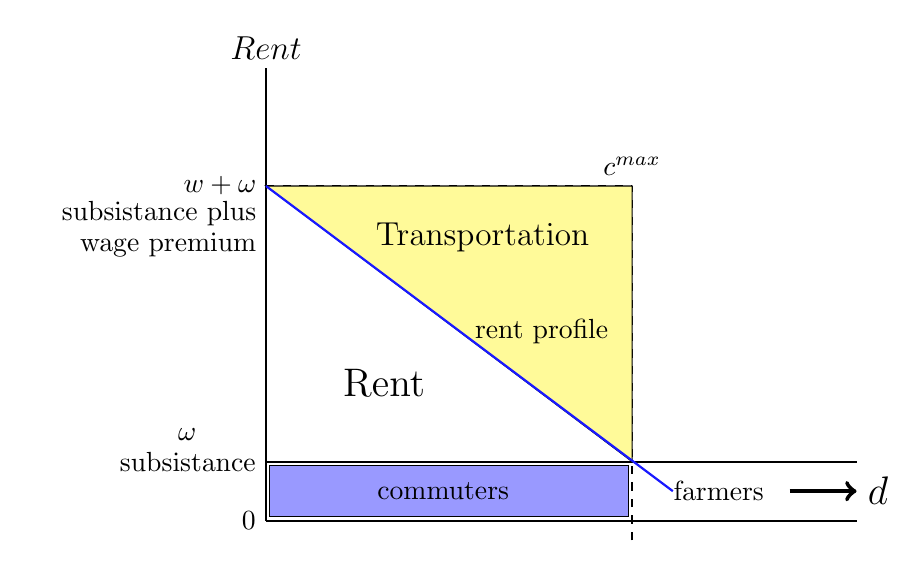
\begin{tikzpicture}[scale=.5]
\def\bndmax{5}        
\def\bndmin{0.2}
\def \n {10}  % height of y axis
\def \d {15}  % length  of x axis
\def \t {.75}  %  cost of transportation per unit x
\def \th {1}   %
\def \w {7}    %  wage premium
\def \om{1.5}%  omega =rural wage Zero for urban population
\def \azero{2}
\def \aprime {-.0}	
\tikzset{func/.style={thick,color=blue!90}}	
\draw [thick] (0,-\om) --(\d,-\om);  			% Zero for rural population
\draw [thick] (0,-\om)node[left]{$0$} --(0,\n);	% Y axis
\node at (0,\n+0.5){\large$Rent$};

\draw [thick] (0,0)node[left]{subsistance}--(\d,0);
\node a t(-2,.7) {$\omega$};
\node[left] at (0,\w){$w+\omega$};
\node[left] at (0,\w-.7){subsistance plus};
\node[left] at (0,\w-1.5){wage premium};	
\draw [dashed, thick](9.3,-2)-- (9.3,\w)node[above]{$c^{max}$};
\draw [dashed, thick](0,\w)-- (9.3,\w);
% solid color for commuters
\draw[fill=blue!40] (0.1,-0.1) rectangle (9.2,-\om+.1);
\draw[fill=yellow!40] (9.30,7.) -- (0,7)--(9.30,0.)--cycle;% Rent \w-.2
\draw[func,domain=0:\w/\t+1] plot [samples=200] (\x,{\w-\t*\x});
\node at (5.5,5.7){\large Transportation};
\node at (7,3.3){rent profile};		%Rent Profile	
\node at (3.,2){\Large Rent}; 		%Rent 
\node at (4.5,-\om/2){commuters};
\node at (11.5,-\om/2){farmers};
\draw [ ultra thick, ->](13.3,-\om/2)--(15, -\om/2)node [right] {\Large $d$};
\end{tikzpicture}
    \caption{A circular city with uniform transportation costs.}
    \label{fig:rent_alonzo}
    \end{center}
\end{figure}

A simple case is the circular city with uniform transportation cost, $t$. \[r^*= \frac{w}{t}\]% A more complex model might have density depend on location, for example, in the continous circular cityt\,
If transportation costs vary by  distance we might have something like this constraint on extent\[w=\int_0^{d*} t(d)dt.\]

This approach imposes an equilibrium condition on the model. It is unnecessary working with a citation of known extent and density. The analytic approach is easily extended to variable transportation cost, although at the expense of additional computational complexity.

\subsubsection{City extent and population}
Equation  four  closes the model by linking the extent of the city to the population. A simple case is the circular city with uniform population $d$, where $d$ is density per unit area and $r^*$ is the radius of the city: \[P=d\pi r^{*2}\] 
More generally, density might vary with for example, the distance $r$ from the centre of the city:
\[P=\pi \int_{0}^{r*}d(r)\,dr\] In a computational model a table of densities would provide the link.


\subsubsection{challenges}
maybe discuss some of the modeling challenges - division of income, lags, ???

\color{black}


\vspace{2cm}


\color{green}
 The growth of many cities was initially fueled by agricultural rents and resource exports. The industrial revolutions transformed many of these consumption cities into thriving production centers. 

while the ``origins'' of consumption cities can be traced to (i)
resource rents, (ii) rents from agricultural exports in countries with sufficiently high agricultural productivity, and (iii) ``premature'' deindustrialization.  Source:
%\href{https://www.brookings.edu/blog/future-development/2022/07/14/1622441/}
{Are cities engines of production or consumption, and does it matter?}








\subsection{Rent seeking}
  Rent-seeking is the act of growing one's existing wealth without creating new wealth by manipulating the social or political environment. Rent-seeking activities have negative effects on the rest of society. They result in reduced economic efficiency through misallocation of resources, reduced wealth creation, lost government revenue, heightened income inequality,


\color{black}
% 

\chapter{Urban Land and Land Rent}
\section{The Alonzo-Jacobs Model}
In 1964, William Alonso published \textbf{Location and Land Use}, in which he described a model that specifically linked the urban wage premium to urban land rents and  became the central model in modern urban economics. 
We use an \textbf{Alonzo-Jacobs model} to explore the source and distribution surplus value, where the reference to Jane Jacobs links the wage premium to Jacobs-style  agglomeration effects that generate urban productivity.% and the wage premium. 

Ricardo had described a model with a central market for corn, producing corn took land and transporting corn to market was costly. Because there is one market price for corn, land with low transportation costs near the central market earns a rent. More distant land has lower value. In Alonzo's model there is central market and a single price for labour, producing labour takes land, and transporting labour to the market is costly. Alonzo simply re-presents Ricardo's conception of rent  mathematically for a different social system and production technology.  

The logic of the model is illustrated in the following figure. The height of the green bar on the left illustrates the premium for urban labour at the centre of an Alonzo circular city. The height red triangle at the left is the rent earned on land at the centre, which has no transportation costs.\footnote{The model says nothing about who gets the rent in the urban economy. For classical economists it was obvious that the agricultural rents went to the class of land-owners.} Transportation to and from the center costs $t$ times the distance $d$ from the center. Fuel, capital, and time costs are  all included in $t$. 


\begin{figure}
    \begin{center}
    
% Simple Alonzo model
%%%%%%%%%%%%%%%%%%%%%%%% PARTITIONING THE LABOUR SHARE
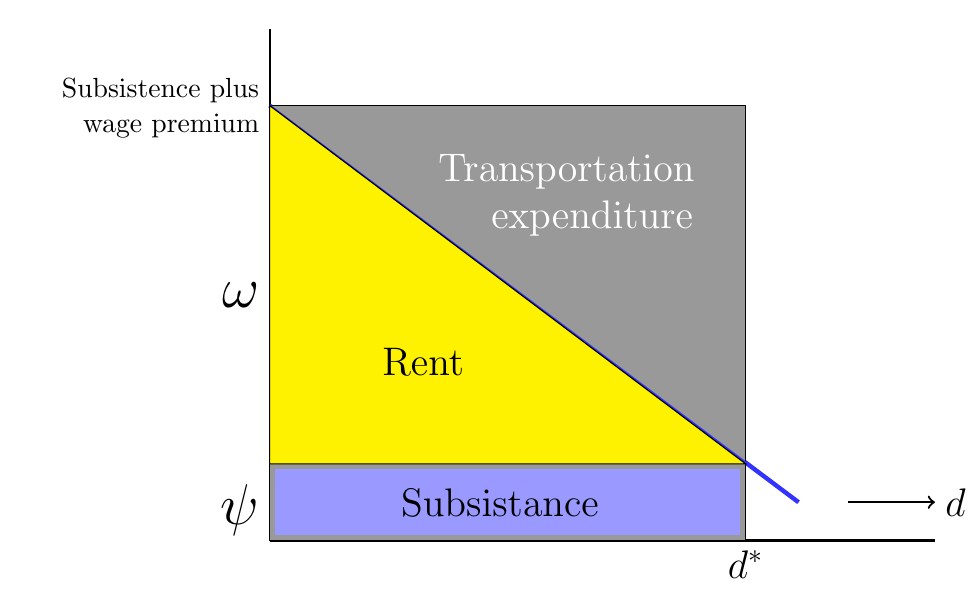
\begin{tikzpicture}[scale=.65]
\def\bndmax{5}        %https://tex.stackexchange.com/questions/68462/filling-a-complex-region-with-tikz
\def\bndmin{0.2}
\def \n {8.5}  % height of y axis
\def \d {13}  % length  of x axis
\def \t {.75}  %  cost of transportation per unit x
\def \th {1}   %
\def \w {7}    %  wage premium
\def \om{1.5}%  omega =rural wage Zero for urban population
\def \azero{2}
\def \aprime {-.0}	
\tikzset{func/.style={thick,color=blue!80}}	

% FIRST FIGURE just axes PARTITIONING THE LABOUR SHARE
\draw [thick] (0,-\om) --(\d,-\om);  			% Zero for rural population
\draw [thick] (0,-\om) --(0,\n); %node[above]{\Huge $w$};	% Y axis
%\node at (0,\n+0.5){\large $Rent$};

% \draw [thick] (0,0)node[left=.5]{Subsistence}--(\d,0);
%\node at(-2,1) {$\omega$};
\node[left=.25] at (0,3.3){\huge $\omega$};
\node[left=.25] at (0,-0.9){\huge $\psi$};
%\node[left=.25] at (0,3){$w+\omega$};
\node[left=.25] at (0,\w+.3){Subsistence plus};
\node[left=.25] at (0,\w-.4){wage premium};	

%\foreach \xi in {0,..., \n} \draw (\xi,0)--(\xi,-.1)node[below=1]{\small$\xi$};
%\foreach \yi in {1,...,\n} \draw (0,\yi)--(-.1,\yi)node[left]{$\yi$};
%\foreach \i in {1,4,9,16} {
%\node at (7,-\om/2){people scattered uniformly across the land  };

%SECOND FIGURE WITH AGGLOMERATION WAGE
%   \pause %  add urban production and net wage PARTITIONING THE LABOUR SHARE
%\draw[fill=white, white] (0.1,-0.1) rectangle (14,-\om+.1);
%\draw [fill=green!80] (-.25, 0) rectangle(.25, \w);
\node[right] at  (.25, \w/2){Added Productivity};
% \node[right, text width = 3cm] at  (10,9){Where does the increase in productivity come from?};
\draw [ thick, ->](11.3,-\om/2)--(13, -\om/2)node [right] {\Large $d$};

%  THIRD FIGURE  add wage profile PARTITIONING THE LABOUR SHARE
% \pause
%\node[right, white, fill=white,  text width = 3cm] at  (10,9){Where does the increase in productivity come from?};
\draw[func, domain=0:\w/\t+1,ultra thick] plot [samples=200] (\x,{\w-\t*\x}); %Net wageprofile  for 
%\node[right, white, fill=white] at  (.25, \w/2){Added Productivity};
%\node[right, fill=white, text width =3.5cm ] at  (1, \w/2){Declining wage  net \\of transportation\\ costs $T(d)$ };

%   FOURTH FIGURE     commuters PARTITIONING THE LABOUR SHARE
%\pause
%\draw[fill=blue!40] (0.1,-0.1) rectangle (9.2,-\om+.1);
%\node at (4.5,-\om/2){commuters};

%   FOURTH FIGURE    wage bill
%\pause %add total new value
\draw[fill=green!40] (0,-\om) rectangle(9.30,\w);% new product
\node at (4.5,\w/2){\Large urban wage bill};

%%   FIFTH FIGURE   distribution
%\pause
%\node at (9,\n){\Large Partitioning the Labour Share};

\draw[fill=black!40] (0,-\om) rectangle (9.30,\w);% new product repeat
\draw[func, domain=0:\w/\t+1] plot [samples=200] (\x,{\w-\t*\x}); %rent profile
\fill[blue!40] (0.1,-0.1) rectangle (9.2,-\om+.1);
\node at (4.5,-\om/2){\Large Subsistance};
\draw[fill=yellow,] (0.,0.) -- (0,7)--(9.30,0.)--cycle;% Rent \w-.2
\node at (3.,2){\Large Rent}; 		%Rent 
\node at (5.8,5.7)[white]{\Large Transportation};
\node at (6.3,4.8)[white]{\Large expenditure};
\node at (9.3,-1.5)[below]{\Large  $d^*$};
% \node at (4.8,\w)[above]{\huge $d^*$};
 \end{tikzpicture}
 

    \caption{}
    \label{fig:city_simple_alonzo}
    \end{center}
\end{figure}



% %%%%%%%%%%%%%%%%%%%%%%%% PARTITIONING THE LABOUR SHARE
The entire rectangle, $\omega$ $\times$ $d^*$, is the surplus generated by urban agglomeration. Urban land rent, which is the residual when transport costs are deducted from the wage premium, declines  with distance $d$ until, at the very edge of the city, $d^*$, t the cost of transportation  consumes the entire wage. Property values are simply the the present discounted value of the rent at any point.

At the bottom of the figure we illustrate the conventional `subsistence wage'  earned by a worker whether in the city or outside of the city.   In most analyses of urban spaces this living wage is simply ignored, since it is the wage premium that generates rents.  It is also common to assume that the labour market and production at the centre takes no space.   


Workers are attracted to the city by the wage premium, $\omega$,  which represents the share of the surplus generated by the city that goes to labour.  The grey triangle represents the amount of the surplus dissipated in travel costs.  

The extent  of the city  $d^*$ is a simply the distance at which total $rt$ transportation cost  is equal to the wage premium
\[d^* t= \omega\]
where $t$ is the unit cost of transportation. In the figure, $-t$ is the slope of the diagonal line dividing rent from transportation expenditure.



 \section{Implications and results from Alonzo's Circular City}
 It is a beautifully simple model that accounts for many features of urban structure and urban history. In this section we describe some of the insights supported by the model. Extensions can incorporate variation in wages, density, transportation costs,  preference, and even building technology and codes. The limitations of the simple, continuous, equilibrium based versions described above can be overcome using agent-based models to model the evolution of complex and much more realistic urban systems. 

 \subsection{The magnitude of Rents and transportation costs}
 From $w$, $t$ and population density we can derive population, wage bill, total rent, transportation costs. The figure above suggest that  half of the urban surplus is spent on transportation, but because the city is circular, the total value of rents can be represented as the volume  \[ V=\frac{1}{3}\pi  d^{*2} \omega \]
of a cone with radius $d^*$ and  height $\omega = td^*$. Substituting out either  $\omega$ or  $d^*$, we find that total rent is  proportional to the \textbf{cube} of either  $d^*$ or $\omega$. 

The total value of wage payments would appear as the volume of cylinder enclosing the cone\footnote{since the wage is the same for each unit of labour no matter where is t is produced (resides).}.  
$V=\pi r^2 \omega$


 \vspace{1cm}

\begin{figure}
    \begin{center}
    
\begin{tikzpicture}[scale=.5]
   %%%%%%%%%%%%%%%%%%%%%%%%%%%%%%%%%%%%%%%%%%%%%%%%
% definitions for schematic
\def\bndmax{5}        %https://tex.stackexchange.com/questions/68462/filling-a-complex-region-with-tikz
\def\bndmin{0.2}
\def \n {10}  % height of y axis
\def \d {12}  % length  of x axis
\def \t {.75}  %  cost of transportation per unit x
\def \th {1}   % theta?
\def \w {7}    %  wage premium
\def \om{1.5}%  omega =rural wage Zero for urban population
\def \azero{2}
\def \aprime {-.0}	
\tikzset{func/.style={thick,color=blue!90}}	

    %%%%%%%%%%%%%%%%%%%%%%%%%%%%%%%%%%%%%%%%%%%%%%%%
% definitions for Cone3
%\node at (0, 2.5){\input{SA_Cone3.tex}};
     \pgfmathsetmacro{\radiush}{9.7};%Cone base radius was 9.6
        \pgfmathsetmacro{\theight}{7.1}%Cone height (negative if you want a inverse cone)
        \pgfmathsetmacro{\cheightp}{.03}%Cut height in percent of cone height

        %Calculating coordinates
        \coordinate (center) at (0,0);
        \pgfmathsetmacro{\radiusv}{.2 * \radiush}; %HORIZONTAL RADIUS
        \coordinate (peak) at ($(center) + (0,\theight)$);     
        \pgfmathsetmacro{\sradiush}{\radiush * (1 - \cheightp)};%ADJUST FOR COVERAGE AT CORNERS
        \pgfmathsetmacro{\sradiusv}{.2 * \sradiush};
   %     \pgfmathsetmacro{\sradiusv} {\sradiusv -.1 };

\coordinate (antipeak) at ($(center) + (0,-\theight)$);  %thanks  %I added this
\coordinate (vert1) at ($(center)+(\radiush,-.2)$);
\coordinate (vert2) at ($(center)-(\radiush,.2)$);
%problem
   
\coordinate (svert1) at ($(vert1)!\cheightp!(peak) +(0.1,.75)$);
\coordinate (svert2) at ($(vert2)!\cheightp!(peak)+(.5,.75)$);  
    % \coordinate (svert3) at ($svert1+(0,\w)$);
    % \coordinate (svert4) at ($vert2)+(0,\w)$);  
    %  \coordinate (svert3) at ($svert1+(0,7)$ );  % Shifting up by W
    % \coordinate (svert4) at ($svert2 + (0,\w)$0;
   %%%%%%%%%%%%%%%%%%%%%%%%%%%%%%%%%%%%%%%%%%%%%%%%


 
%\draw[step=.5,black,thin] (-9.6,0) grid (9.6,7);
 
% Cone Drawing    
 \fill[ left color=red!70, right color=red!70,  opacity=20,middle color=red!20,shading=axis] (svert1) -- (peak) -- (svert2) arc (170:370:\sradiush cm and \sradiusv cm);

    % FAT GREEN BAR
 \draw [fill=green,opacity=80] (-.2, 0) rectangle(.2, \w);
 \node[above] at (0,\w){$\omega$};
 
%Uncomment this for top of cylinder
      \fill[inner color=gray!2,outer color=gray!40,shading=radial,opacity=.5] ($(center) + (.35,\theight)$ ) circle (9.4 cm and 1.55 cm );
      
        % \draw [thick]($(svert1) +(.3,-.3)$)-- ++ (90:\w-.2);
        % \draw [thick]($(svert2)-(.2,.3)$)-- ++ (90:\w-.2);
        %Lines, \h in percent of cone height
 def \sradiusv2 \sradiusv cm -.1 cm)
% Cylinder drawing
  \fill[ left color=black!50, right color=red!30,  middle color=red!30,shading=axis,opacity=.2]  (-9.05,.5) 
  arc (180:360:\sradiush cm and \sradiusv cm)-- ++(90:\w-.2) 
  arc (360:180:\sradiush cm and \sradiusv2 cm -.1 cm)--(-9.05,.5);  

   \node[above] at (0,\w){\Large $\omega$};
% TRY TO Make a cylinder
%\draw ($svert2 + (0,\theight)$) [arc (180:360:\sradiush cm and \sradiusv cm)]; 
%     \fill[left color=gray!70,right color=gray!70,middle color=gray!30,shading=axis] (vert1) -- (svert1) arc (0:-180:\sradiush cm and \sradiusv cm) -- (vert2) arc (180:360:\radiush cm and \radiusv cm);

% DASHED LINE AT BACK OF CONE
\foreach \h in {0.03}{   %.38,.34,.30, .7
            \pgfmathsetmacro{\rh}{-\radiush * (1 - \h)}
            \pgfmathsetmacro{\rv}{.2 * \rh}
            \draw[black!70,densely dashed] ($(svert2)!\h!(peak)-(.3,.9)$) arc (370:170:\rh cm and \rv cm);%$(vert2)!\h!(peak)$)
        }
  %      \draw[opacity=.90, line width=.05cm, green] (0,0)--(0,{\theight - .05});
%     \foreach \h in {0, .38,.34,.30, .7}{
%            \pgfmathsetmacro{\rh}{\radiush * (1 - \h)} %            \pgfmathsetmacro{\rv}{.2 * \rh}
%            \draw[black!70,densely dashed] ($(antipeak)!\h!(vert2)$) arc (180:360:\rh cm and \rv cm);
%   }
%  \draw[red] (antipeak) arc (30:60:3);
%  \draw[dashed, thick] arc (0:-180:\sradiush cm and \sradiusv cm) -- (vert2) arc (180:360:\radiush cm and \radiusv cm);
%%%%%%%%%%%%%%%%%%%%%%%%%%%%%%%%%

% %\foreach \xi in {0,..., \n} \draw (\xi,0)--(\xi,-.1)node[below=1]{\small$\xi$};
% %\foreach \yi in {1,...,\n} \draw (0,\yi)--(-.1,\yi)node[left]{$\yi$};
% %\foreach \i in {1,4,9,16} {
% %\node at (7,-\om/2){people scattered uniformly across the land  };

% %SECOND FIGURE WITH AGGLOMERATION WAGE
% %  add urban production and net wage
% %\draw[fill=white, white] (0.1,-0.1) rectangle (14,-\om+.1);

% \node[right, text width=4cm] at  (3, \w+1){Added Productivity due to agglomeration};
% %\node[right, text width = 3cm] at  (10,9){Where does the increase in productivity come from?};
 \draw [ thick, ->](0,0)--(2.5, 0)node [right] {\Large $d$};


% \draw[thick] (0,0) -- ++ (50:2.6cm);  %   diagonal for perspective
% \draw[thick] (0,0) -- ++ (230:2.35cm); 

% %  THIRD FIGURE  add RENT profile in blue

% %\node[right, white, fill=white,  text width = 3cm] at  (10,9){Where does the increase in productivity come from?};
% \draw[func, domain=0:\w/\t+1,ultra thick] plot [samples=200] (\x,{\w-\t*\x}); %Net wageprofile  for 
% %\node[right, white, fill=white] at  (.25, \w/2){Added Productivity};
% %\node[right, fill=white, text width =3.5cm ] at  (1, \w/2){Declining wage  net \\of transportation\\ costs $T(d)$ };
% %\node[right, fill=white, text width =3.5cm ] at  (4,9){Declining wage  net \\of transportation\\ costs  };
% %
% %\node at (0, 1.5){\includegraphics{\input{SA_Cone3.tex}} };
% %\node at (0, 2.5){\input{SA_Cone3.tex}};

% %   FOURTH FIGURE     commuters
% %\pause
% %\draw[fill=blue!40] (0.1,-0.1) rectangle (9.2,-\om+.1);
% \node at (4.5,.4*\om){commuters};


\end{tikzpicture}
    \caption{}
    \label{fig:city_conical}
    \end{center}
\end{figure}




 \vspace{1cm}
and total transport costs are 
$\frac{2}{3}\pi  d^{*2} \omega).$
With uniform density, population is proportional to the square of  $d^{*2}$ while rents and  transportation costs are proportional to the cube. 

\subsection {Changing Transportation Costs}



 It is easy to see that the transportation cost revolution brought about by first street cars and later automobiles made much larger cities possible.  It also affected social structure and left indelible marks of the form of cities developing at the time and after.In North America, with large amounts of land, it generated massive urban sprawl, but also made land available for a growing `middle class.' Ultimately it generated congestion and rising transportation cost that began to limit urban growth. 

\section{Adding Jacobs-style agglomeration effects}
Rising urban productivity will raise the wage, attracting more workers. If they are added in suburbs at the edge of the city (Ricardo's extensive margin) virtually all of the wage premium they receive is dissipated in transportation costs. Closer to the centre,  land rents rise. Owner-occupiers capture the increase as property value appreciation. Tenants are likely to be faced with higher rents.      

If agglomeration is the source of productivity gains, however, the new workers increase the urban premium, further increasing land values and attracting more workers. 

% \chapter{Financialization}
% \chapter{Model}
\label{Sec:Model}
%MAIN VERSION HERE IN OVERLEAF UNTIL MOVED BACK

%We build a spatially explicit agent model where agents work in one location and have transportation costs to travel to work. 

This work integrates a model of production and labour into a standard spatial model of the city. 
In this chapter, we introduce an analytic model of production and a labour market in a stylized circular city. 
We develop a spatial model with a labour market and agglomeration effects consistent with the literature as our base model. 
% Extended appropriately, this basic model could be used for planning.
We take a step beyond integrating labour markets in a city, to studying the distributional effects: who gets the surplus, what does that mean for the class structure, and ultimately the productivity of cities? 
% In this section we introduce the production function, introduce the labour supply and the urban model, the source of the surplus, then we calculate profit, consider who gets the profit, and from there we draw our conclusions.. then we calculate the urban surplus, and consider who gets it. 
%In subsequent sections we relax assumptions and look at how the interaction between the production of social wealth in cities interacts with housing and the extraction of rent to drive patterns in a richer model with heterogenous agents interacting over space and time. 
In the next chapter we will integrate a version of this production model in a spatially explicit agent based model with financialized investment. 

This model has two parts, first a production function, modelling how urban regions generate wealth, and second a model of an urban housing market. 
In this section, we introduce the basic structure of the model and examine the effect of agglomeration, using a circular city model.  
\textbf{The model has a Solow-Swan style production model with agglomeration effects using a Cobb-Douglas production function that incorporates Jacobs-style labour-augmenting agglomeration economies 
%(Beaudry and Schiauerova 2009, Panne 2004, J. Jacobs 1969), 
in the way neoclassical growth theory incorporates labour-augmenting technical change.}
It then integrates the production function with an Alonso-style urban model of a city economy (Alonso 1964). 
It is a model of a productive economy since the centre is productive and demands labour.

% Alternative phrasing 
%We integrate a labour market into a spatial urban model, set up to explore rent, and implications for the distribution of wealth.
%This model has two parts, first a production function, modelling how urban regions generate wealth, and second a model of an urban housing market. In this section introduce the labour supply and the urban model, we model the production function, then we calculate profit, consider who gets the profit, and draw conclusions. % The work draws on the Alfonso/Von Thünen model of the concentric city and Dawn Parker and Filatova's work in agent based modelling of housing markets (see http://jasss.soc.surrey.ac.uk/12/1/3.html 2009).% We begin with a simple model of a circular city with urban agglomeration effects. In subsequent sections we will use an agent based model to relax assumptions to look at how the interaction between the production of social wealth in cities interacts with housing and the extraction of rent to drive patterns for individuals over space and time.

The result is a simple model in which marginal productivity determines the wage, the wage determines the size of the city, the size of the city determines the labour supply, and labour supply determines marginal productivity. 
The model is constructed so that there is neither land rent nor capitalist exploitation in the rural economy. 
This special case allows us to examine the distribution of the social surplus generated by agglomeration economies and the effect of financialization.

In the simplest model, the central place pays a uniform wage, $w$ to all employees, who have identical preferences and transportation costs. $w$ is an attribute of individual residents. Residents  purchase or rent equal quantities of land at differing locations $l$ for identical housing.  

There are transportation costs $T$ that depend on distance from the  central place, so land close to the central place is more attractive than land farther from the central place.  

The equilibrium concept is that a market with identical individuals with identical incomes and transportation costs will result in identical utilities. The result is that land rent must decline with distance from the central place to offset rising transportation cost. 

The size of the city is determined by population and lot size. Income and transportation costs will interact with lot size. The basic model can be initialized by matching the number of properties to the size of the population. 


\subsection{A Circular City}

%Call it a radial city?
Following the Alonzo model [], firms are located at the centre of a circular city, the central business district. Residents residents live, spread across the space, and can take jobs and commute to work.
%In the simplest version, firms concentrate at the city centre. Workers are spread over space and pay transportation costs to commute.

Firms produce goods to sell. They can produce more goods by hiring additional workers. 
There is an agglomeration effect, which means firms can also produce more goods by operating in a city with more people, because of the connections and interactions between people (CITE). 
The simple circular city can be extended to to produce other forms, including polycentric cities and hierarchies of cities at the cost of additional computational complexity. The simple case we examine will allows us to focus on the general, and neglected, distributional features of this class of models.

\subsection{Labour Supply}

%The wage  determines how far people can travel, since it pays for subsistence, that surplus can go to travel, so the higher the wage, the farther workers travel for work. \note{Maybe } 

Workers in the countryside receive a subsistence wage, $\psi$, which could come from work in the local community, living off the land, family support, social support, or something else. % cite other models with subsistence wage.

Firms pay a wage premium, $w$, over the subsistence wage to attract workers. 
When workers take a job, they give up the subsistence income and instead receive the wage from their employer. 
The total wage employers pay is thus the subsistence wage plus the urban wage premium  $\psi + w$.
Specifying the model in terms of a wage premium simplifies the link to the production side and the treatment of household choice.

The urban wage premium determines how far people can travel. The higher the wage, the farther workers travel for work. 
Workers will go to work if the wage premium is greater than the cost of travel, $\tau$ per unit distance. 
Wage and transportation cost therefor determine the radius of the circular city, which determines the size of the labour force which affects urban productivity.  The cost of travel is therefore an important variable in the development of urban productivity. 

%Living close to work has value to workers because it saves the cost of transportation. 
%We assume workers receive a subsistence wage, $\psi$, in the countryside, which could come from work in the local community, living off the land, family support, social support, or something else. % [MAYBE ADD This follows xyz's approach, and makes it possible to explore resident's choice to work]. 

%If the cost of transportation is $\tau$ per unit distance, then t
The farthest workers will travel to work is thus $\frac{w}{\tau}$, which defines the radius of the commuter shed. Thus a worker, located at a distance $d$ from work, paying as much as $w-\tau d$ in rent, would still choose to work, and the maximum distance that workers will commute is the radius of the commuter shed. Given a uniform lot size $s$, with one worker per unit land, the labour available is the area of the city. In the circular city, this is the area of the circle divided by the lot size
\begin{equation}
                 L%=  \frac{\pi}{s}(c^{max})^2	
			=\frac{\pi}{s}  \left(\frac{w}{\tau}\right)^2
			=\frac{\pi}{\tau^2 s} w^2, \label{Eqn:LabourSupply}
\end{equation}
which increases with the square of the wage. This is the equilibrium urban labour supply curve.

As in the standard circular city model the constraint on city size and hence growth is provided by transportation costs, which limit the size of the labour force at any wage. 
% Rising transportation costs can become the limit on firm or city expansion. 

%To get wage, we can write thee  inverse labour supply function  is
%\begin{equation}
%	w= (\frac{ \tau^2s}{\pi})^{0.5} L^{0.5},	%\label{Eqn:InverseLabourSupply}
%\end{equation}

 % TODO:  FOOTNOTE the transportation cost/distance relationship appears to be non-linear in many cases. While the linear model connects with the established literature, we likely want to explore the implications of more empirically grounded curve (e.g. Alain Bertaud, 2015)
% More generally, if we were to introduce variations in lot size and housing types  we would want the integral of the worker density function. In our ABM version  of the model we simply count the workers within the commuter shed.

% DETAILS AND ALTERNATIVE PHRASING  
% MARGINAL PRODUCT The marginal product of labour is monotonically declining, ensuring a labour market equilibrium, to connect with the analytic tradition of economic modelling by ensuring there is an equilibrium level of production.  While adding more labour may always adds some value, the rate at which it adds value drops off. 
% If the marginal product increased, then a firm that got large enough would out compete smaller firms, hire all labour, always be able to produce more wealth by hiring more people, and would always produce more wealth by hiring people than by firing people. This doesn't happen. 
% Perhaps, the firm hires employees who best fit its needs first, but to grow, eventually it must hire less selectively. Finding markets may get harder with growth. Perhaps expansion adds additional costs, building a parking lot, administration, acquiring a larger building. Whatever the explanation, the marginal product of labour declines. 

% Frictional unemployment usually just refers to people moving between jobs. When people look for jobs, it may take time to get them. The analytic model offers an equilibrium solution with full employment. In the agent based model this assumption does not hold, workers are laid off, and take time to find new employment.
% labour adjustment costs include moving costs for the employee or hiring, firing, or training cost for the firm. (there might be a hiring, firing, or training cost on the firm side, or on the employee side: expected time to employment costs, moving costs, etc.)
% The assumption of monotonically embedded marginal product of labour is embedded in the production function, so it applies in the analytic and agent models. This appears in the requirement that the sum of the exponents in the Cobb Douglass are less than one without agglomeration effects. Agglomeration effects can push the sum above one. When the exponents add up to less than one, there are diminishing returns to scale.  Exploring alternatives would involved exploring other formulations of the production function.

% $mvp(x) = p(x)$ where x can be labour, capital or any other factor, falls out of the function when you introduce profit maximization. Continuity and differentiability assumed but it is a convenient approximation-- take away assumptions you typically get a close approximation.

%We have a two factor model of production with labour and capital.  


\subsection{Production}

Firms produce goods which they sell in a commodity market\footnote{For simplicity, assume firms produce a variety of perfectly substitutable commodities which are exported and locally consumed at a fixed price in a large market. Note increasing product variety may produce a consumption agglomeration economies as in \cite{FujitaKrugmanVenables}.}. Demand for the urban product is perfectly elastic which means producing more won't affect the product's price; and there are decreasing returns to scale, which means each new worker increases output by less than the last worker did. 
  
We use a two factor model of production, where production, is a function of capital and labour. The firm maximizes profit by setting the marginal value of the product of each factor equal to the unit cost per factor. We model agglomeration with a Solow-Swan style term for labour augmenting technical change. In the Solow-Swan model 

 \begin{equation} 
Y(t)=K(t)^{\alpha }(A(t)L(t))^{\beta }
\label{Eqn:Solow-Swann}
 \end{equation}
where $Y$, $K$ and $L$ are aggregate output, capital, and labour, respectively,  $A$ is the term the Solow-Swan model introduced for technology, that can capture the growth of labour productivity over time, $\alpha$ is the elasticity of output with respect to capital, $\beta$ the elasticity of output with respect to effective labour, and $t$ time. If $\beta=1-\alpha$, this is a constant returns to scale (CRS) production function at the firm level.

% In the Solow-Swan model all factors of production are fully employed, and initial values $A ( 0 )$, $K(0)$, and $n( 0 )$  are given. The number of workers, i.e. labor, as well as the  level of technology grows exogenously at rate %s are $n$ and it   $g$,% respectively:     $L(t)=L(0)e^{nt}$     $A(t)=A(0)e^{gn}$ 
 
This model uses a similar functional form to look at  the effect of population density increasing % productivity. %how density increases in in  % It models how population increases productivity. $\Lambda(n)n$ is  ``effective labor'' 
 the productivity of labour, rather than technology growing productivity over time. With labour augmenting agglomeration, $\Lambda(n)$, in place of technology, the equation becomes 

\begin{equation} 
Y=K_i^{\alpha }(\Lambda(n)n_i)^{\beta }.
\label{Eqn:Prod1}
\end{equation} 
where $n_i$ is the number of workers at the firm, the labour, and $n$ is the urban population. The agglomeration factor increases with population. It multiplies labour because agglomeration scales the productivity of workers. 

A natural functional form of the agglomeration effect for illustrative purposes n is $\Lambda(n) = n^\gamma$. Then:

\begin{eqnarray}
 Y&=K^{\alpha }(n^{\gamma}n)^{\beta}  \nonumber\\
 Y&=K^{\alpha }n^{\beta(1 + \gamma)}.
 \label{Eqn:Prod2}
\end{eqnarray}
If $\gamma=0$ there are not agglomeration effects. Notice that  this formulation implies it is possible to have increasing returns to scale for the urban economy even with a production function at the firm level with decreasing returns to scale: the return to the total economy $\alpha + \beta(1 + \gamma)$ can be greater than one, even if $\alpha +\beta$ is less than one. %.\label{Fn:PSI}}  
(CITE Appendix: Excess Returns)

Assume $\Lambda(1)=1$ so the agglomeration effect has no influence with one person in a multiplicative function like the Cobb-Douglas, and %$\die
FIX die ${\Lambda}{n}>0$, so it is increasing with population.

%%%%%%%%%. ***WHY
If $\beta=1-\alpha$, this is a constant returns to scale (CRS) production function. Without agglomeration effects, $T(n)=1$,  Then  \textbf{$\mathbf{L(n) = T(n) n}$} 

% Without agglomeration effects, $\Lambda(n)=1$,  Then  \textbf{$\mathbf{L(n) = T(n) n}$} }

% Firms will purchase the time of workers to capture the product of their effective labour % and enjoy the product of effective labour. %was If labour markets are competitive, it will set 
%$\die{Y}{L}=w$.
%*** DEFINE EFFECTIVE LABOUR, COMPETITIVE MARKET
% Effective labour is the productive output from labour. As soon as you introduce agglomeration economies, labour becomes a more complex phenomena. There is the benefit of the single worker which should be perfectly declining on that nice concave production function and there is the diagonal movement as a result of increasing productivity because you keep adding people to the market. That means that your productivity of the worker isn't' just attached to the worker and your plant. It has this other component.. 'effective labour' -- the output including the A term.
% Labour always depends on the human capacity, technology, tasks aside so it is always complicated
%Capital is always complicated too it has dates, whether you can get the inputs for it, whether they're produced nearby etc.. -- 

%** ``The notion that your labour force is on average more productive when there are more people around is pretty dramatic and it's very much not part of the basic model that we use. Our starting point is that's the fundamental feature of cities, and what does that do with financial capital and what does that do to distribution and that's not been explored.

%Competitive market- everybody is a price taker they don't assume.
%price takers don't assume anything you do affects other producers or suppliers .. so you act in terms of account your internal prices and costs.
%Take into account any one else's behaviour
%the easy way to see that is assume prices are fixed - all that's required to get the behaviour.

%* have a few other things like free exit and entry, perfect information etc -- to get the efficiency result. - (or to ensure price taking)

%Monopolists knows that increasing output will require a reduction in price-- and take into account how consumers will apply and take it into account.
%No externalities imperfect information etc.. ensure efficiency but aren't needed, all you need is price taking for individuals to only pay attention to their own costs and their own benefits. 

%competitive markets many sellers, many buyers, monopoly single seller, monopsony - single buyer, intermediate cases - monopolistic competition - with some market power but not complete - duopoly- some inefficiency depending on the behavioural model because in the duopoly case they may be able to take advantage of the behaviour of buyers.
% Start with perfect competition, then introduce monopolistic competition is most likely.. but it's more difficult to handle. e.g. with brand names, people have some preference for some feature of your particular good so you can price it higher even though you may loose some marginal people. Firms compete on brand name and reputation, not the pure cost effect.
% In the spatial economy, goods are deferentially interchangeable. Put them on a line and firms pick a place along they line. Firms are in competition but are competing on a line-.. spatial model moved over to characteristic space.. -- looking at this would involve overlaying another space - the characteristic space on the physical space. .. There are also local places with local grocery stores. Polycentric stores have effectively monopolistic competition in real space. - like a named cafe downtown has the same.
% Market power means you can price above marginal costs. Need free entry to get rid of it. -- it doesn't drive out profit - profits can be sustained over longer.
% Monopolist can charge a higher price but pays competitive price for all inputs including labour. If a firm also had a monopoly on offering jobs, they could drive down wages.

%Firms calculate what the next worker is worth to them. That's what they're willing to pay for labour. 
%This is the labour demand function based on the marginal product which is declining. When a firm has only a few workers, it is high on that demand function, and has to move down. It cuts workers. If it's too low, it expands and hires. Note this says something about the geometry of what employers could pay. Firms can't pay workers more than they can earn in the long term, unless that money comes from somewhere, but they could push down wages and extract more profit, invest more in other factors of production, etc

To maximize profit 
% firms set the marginal value product of labour, $p\die{Y_i}{n_i}$, equal to the wage. 
in a competitive market, firms offer a wage equal to marginal value of labour, 
%$p\die
FIX p die ${Y_i}{n_i}$, where $i$ indicates the $i^{th}$ firm. In the analytic model, there is no frictional unemployment, there are no labour adjustment costs.\footnote{Note: we do not assume equilibrium conditions in the agent model, however our approach is to stay close to the analytic tradition, relaxing assumptions to clarify what drives each results, and connect the work with classical and neo-classical theory.}. % For instance in the agent model, employees are simply laid off and seek work, so there is unemployment, but there are not labour adjustment costs for firms.}. For convenience, price per unit is one. 

A labour market equilibrium exists if the marginal product of labour, is monotonically declining, which it is with a Cobb Douglas production function, and $\alpha + \beta<1$ 
Population would be expected to adjust much more slowly than firm wages, so labour supply should converge. The case where there are increasing returns at the city level introduces interesting dynamics, explored in appendix CITE % 'furthur discussion' appendix.

%To ensure there is a labour market equilibrium to study in the analytic model, the marginal product of labour declines monotonically, 
%***ILLUSTRATE AND CLARIFY
%If you see it as just supply and demand .. 
%Supply demand with fixed product and everything’s neat
%Agglomeration changes everything,.. firms are underestimating each time they add a worker, the value that’s going to be produced. They benefit from an agglomeration effect and that’s where they interesting dynamics are coming from..
% we know that there is a marginal product of labour for a firm that it should be able to figure it out.. can the person on the shop floor figure out whether it's worth hiring another person.. we can talk about it, add details etc. We have a declining marginal product of labour. Because of transportation costs, we have a rising cost of getting labour so they cross and there is an equilibrium. There are adjustment questions like which adjusts quickly, how fast people move in, how fast firms decide to hire etc, but we know that there is in principle and equilibrium and that it is in principle a stable equilibrium (DIAGRAM STROGATS) although there are complications with this-- some argue these market equilibria never make sense- true in lots of way, but useful for analysis. 
% The question is then, what happens in our city? Do you get a growth dynamic? What seems to be the case is that if all the firms add workers then the marginal value of the product of all the workers they have goes up, which means they are making more profit which means if they are making more profit they want to hire more workers? Does it ever converge? Likely eventually, but it's got a very powerful dynamic.  If you add other features like more products being created in the city, which is part of this agglomeration process you can start seeing, if you exhaust one source of growth, we know that there are others, that simplification is just firms of the same sort hiring workers of the same sort is wrong. so we need to add the local service sector, we need to add the possibility of creating new products and those depends on the number of workers and so depend on further agglomeration effects. What does this mean? For the purpose of the model, we'd want to strengthen the agglomeration effect relative to what they are for specific firms or industries..

Population/workforce, $n$, and the wage will be determined endogenously in competitive markets. 


 \subsection{Rent}
\label{Sec:Rent}

%``We model how land rent is captured by landowners and how that affects wealth creation and the development of the city. 

%Land is a monopoly good \note{talk about what you mean by monopoly good?} 
The supply of land at any distance from the center is inelastic. 
Its value comes from proximity to the productive urban centre, not from the value of improvements made to the property. 
% Reference sections on development which is different, and the contribution of amenity % Because supply is fixed for urban land, and the landowner has a monopoly claim on rents, the rents that can be depend on wages and amenity rather than the cost of improvements made to the property.
% The source of rents is the free gifts of nature, the coming together of people to create value in cities, and the concentration of public amenity in cities. 
In the circular city with linear transportation costs, the maximum rent for living closer to work is at distance $r$, from the center, is $w-\tau r$.  is Workers could pay that much and it would still be worthwhile to commute to work. 

Rents go to landowners. %the owners of a given property. 
Landowners therefore capture a fraction of the wage premium generated by agglomeration.

If workers own their own homes, rents go to them. If others own the land, they capture them. %\note{REPHRASE? rent is  extracted from the coalition of capital and workers.} % Rents may also be taxed, could be shared between multiple owners, etc. 
%The rents are captured by landowners.  The capture of rents by landowners is common buy not necessary. 
In principle the gains from urban productivity and amenity can be allocated as social wealth through shared ownership, as is often done on a small scale with cooperatives and land trusts, distributed to all citizens through something like a social wealth fund, or captured in taxes or fees as Henry George suggested. 
%The rents would otherwise go to labour and capital.

% Agglomeration benefits get extracted by landowners. Labour gets only their marginal value they don't get any of the surplus. They don't even keep always their marginal value.
the dynamic story is that the class of landowners eventually becomes financial capital.
PLOT RENTS HERE

The value of land increases over time. Those who purchase land earlier claim a share of the growing value of the city. % As the city grows, they own an increasingly valuable asset.
 
%In this model, workers are the initial owners, but they build this wealth which becomes a source of capital that can support them.

EQUATION FOR THE SHARE THEY CAN CAPTURE


\subsection{Demographics}

Workers can leave the workforce and retire, and new people can come into the city. Land value rise as the city grows, so newcomers pay more for housing near the centre.

In the case in which individual workers purchase houses and then sell them on retirement, the housing market drives the creation of classes on its own. A strictly random process in which agents have a range of ages and sell at retirement creates a structural advantage where workers who arrive earlier in the city and own land, benefit from their own labour but also get to claim a share fo the productive output of the city as it grows. % those who begin work later. % to a division in wealth
%the emergence of a class of those who came early and those who came late.
%Early agents may also rent out their land. Could it be though of as a pyramid scheme?

In the classical language, someone is exploited if someone else gets a share of the value of their labour. %(REPLACE WITH MORE PRECISE DESCRIPTION). 
 Employers capture a share of the value of workers' labour, so they exploit workers under this definition.
Those who own land early in a growing city are also capture a share of everybody's production. Since they capture a share of the productivity of others working in the city, through the rents, they are also exploiters, they form a kind of hybrid class. %Rents could be captured directly through renting out the property after they retire away from the city,  or by selling the property at a higher value than they bought it. 

% MARGINALIST DISTRIBUTION
%we've been paying some people less than the market wage so our profits our higher. this is what it would be if we paid everybody
% FOOTNOTE - RELATIONSHIP with marginalist distribution story ******** TODO Does the marginalist approach assume they are not exploited? Is it an experiment in examining the case where production is non-exploitative? 
% In a sense if labour gets the marginal value of their product, are they exploited. It's a matter of interpretation.  -It has an attraction 
%Clark tried to make an ethic of this. if everyone is being paid the marginal product of their labour. We know that's an efficient outcome. If it's efficient, is it also fair
%Is it possible someone's taking out an extra large fair. Yes. Not fair for simple classical reason that labour has been exploited in the past and that the current owner ship is a result of exploitation. The ownership of land introduces a kind of exploitation-- clearly exploitation if you claim that. 
%Lot's of marxists didn't like Henry George making it a locational question, they wanted to keep it located in the factory.
% You could - well what value did they create -- in line with those other-- could interpret.. 
%What is the average value, because every worker is not just marginal, they're also average/identical. What is the value created by the whole of the workforce. Should they be paid the marginal value or the average value of their work.
%
%The avg value -- declining.. 
%The demand for labour is declining--  
%Every infra marginal worker has been paid less than the avg contribution 
%Every infra marginal workers should - 
%every marginal worker should get the average wage.. that's fair.
%
%Get to the margin - that's what you pay.. that's what the next worker is worth to the firm. .. 5th' worker is paid more than the 10th. should it be averaged out and paid to all workers? paid to worker, or should the difference between top and the marginal goes to the firm- -- that's profit.. pay everyone the marginal value and keep the rest as profit.. 
%Effective labour has a higher marginal product.. - even higher - higher for the firm.. - but they don't have to pay the workers that... firms only have to pay enough to get their marginal individual cost down to the wage. The problem there is if they're making more profit they want to expand the workforce, but that wage only supports a certain size of city -- they've got off raise the wage a bit.. so they face an upward sloping supply curve for labour=-- that's why you know there's an equilibrium.. declining product and upward sloping supply so they cross.
%
%(all the profit you earn on the way could be redistributed)

\section{Chapter: Land Market}

Urban productivity %and amenity
drives land values through the housing market.%Agents purchase homes to live in. The value of the the proximity to work and to amenity drives shapes the what agents are willing to pay. 
% These prices shape the relationship between housing markets and the wealth of households.
Our goal is to look at the relationship between housing markets, financialized investment, and production. % and labour markets. 
To explore this relationship, we integrate the model of production developed above with a spatially explicit agent based land market. % in which heterogenous individuals and institutions buy and sell properties given their individual goals, resources and available information. We integrate this housing market with % within this model of individual and institutional actors in a spatially explicit property market, a model of production and employment.

We examine the effect of housing on wealth inequality by looking at 
%We explore the wealth forming dynamics of the urban agglomeration effect by modelling 
a city in which agents work in the city and leave their jobs when they reach retirement age. They may choose to rent or sell their home. %?They may chose whether to stay in the city, if there is sufficient amenity value for them, to rent their house, or to sell it. % Todo can agents choose not to retire? Can they keep working? Do they get the subsistence wage on retirement? Do they need to leave the city to get it? 
New agents enter the city to work. 
Agents fund their retirement from savings, as well as returns on their home if they own one. Savings may be invested in a pension fund, or in local property,  depending on expected risks and returns. % either in the stock market, or in pensions.
A financial institution manages the pension, investing in the market or in property.
%Institutional and individual investors can access debt. %We also consider a case where outside money can come under institutional management, not just local retirement savings. A parameter controls the inflow of additional money beyond local investment in the pension fund. 

% There is an outside world in two respects. There is a market for the urban product produced by firms, and a financial market that agents can invest in.
% Lots of simple extensions e.g. 2 cities with immigration, differentiated labour, products, market power, neighbourhood effects (see extensions map/typology), we focus on those elements central to seeing the structure of the resilience dynamics of the wealth/housing effect. Consider adding density, to look at how it interacts with agglomeration effects. (integrating with transportation effects is very neat)
 
 If there is a housing market, agents can move. %In the analytic case above, the population stays in place, and travels to work if it is worthwhile given the transportation costs. 
%Those who come to the city will be those for whom the benefits the city offers make it worthwhile to  whether that's building their network, accessing markets, accessing amenity, learning, finding specialized employment, or increased wages. In this model 
The demand for labour drives urban growth. % The housing market depends on how many people from the periphery are completing to claim places in the city. TODO IF ANY RURAL AGENT COULD MOVE IF THE CITY HAS ADDITIONAL DEMAND FOR LABOUR, HOW DO WE DECIDE WHICH DO? Could use a parameter for immigration (or how 'hot' the market is) and in the simplest case (corresponding to how many agents from outside are looking at the housing/rental market), have the inflow match. % Agents have debt and there is an undifferentiated labour market
 % We may. 
 
Figure xyz traces the flow. In each time step agents firms update wages and job availability, agents decide whether to work and whether to buy and sell homes.
 % Schedule: Multi step by breed
 % Steps Labour
 % step - workers: market/production, enter market to buy, list properties real estate agent matches agents - has bids 
 % bidding - workers and firm consider properties and make bids (2nd step or spread over 2 steps)
 % negotiation - sellers consider and accept bids (or real estate agents manage negotiation)
%Buyers evaluate their need for housing.
% Agents decide whether to enter the housing market as a renter or a buyer.


 
Worker agents from outside the city can always consider moving and accepting a job. % QUESTION - how to manage the flow of new agents?
%, or can make more from rents and moving away (with a non-differentiated workforce)
% They need to approximate housing prices to know if it makes sense to work. Do they use past prices?
% 
% 
The higher their need, the more houses an agent considers, and the more willing they are to negotiate on price. % Buyers rank their housing need on a scale of one to ten. 
% Maybe later: Buyers could consider neighbourhood pressures, demographic changes, changes in job location, desire for amenity etc. in their assessment of housing need. 
Buyers then consult with a financial agent to determine the maximum mortgage and interest rate they'd qualify for based on their income. This gives an upper bound to the range of homes they may consider. 

Next buyers request a selection of homes to consider from a real estate agent. Those with higher need for housing look at more homes. The real estate agent offers a selection of homes based on the agent's requirements. A randomness parameter determines how many divergent houses are also considered. When the parameter is 1, the selection of homes is fully randomized, When it is 0, the agent sorts all available homes and offers those which fit the agents budget, space, and other requirements best.

Finally agents rank all the homes offered and place bids.  For simplicity of implementation, they place bids on all homes they consider. They place the most competitive bids on those homes they prefer. If they have higher urgency they place strong bids on more homes. 
A utility function/algorithm specifies agents preferences over the attributes that matter. - algorithmic continuous. lexographic- any traits. 

Finally Variables from last time also affect desire and urgency in the next time step. If there is a good fit/price ratio, their assessment of desire increases. If they dislike what they see, their desire decreases -- they settle for what is there. 



%Calculate willingness to pay
%Consider options
%Place bids
%
%Calculate willingness to pay (urgency/position on the market)
%Assess need for housing
%- Urgency of need Unhoused, sold house or served notice? 
%- Family or demographic changes
%- Financial viability of current situation
%Assess financial situation
%Get Max mortgage and max carrying cost given income and wealth from a bank
%Get options from real estate agent
%Place bids based on xy
%Consider options
%Place bids
%
%
%
%BUYER
%
%Enter market to buy
%Decide level of urgency (or decide with prospect theory - functional form for optimism/urgency/time to choose)
%(income/wealth)
%Maximum mortgage 
%Maximum carrying cost
%Household attributes - household size, employment location, amenity
%Current housing
%
%Realtor gives list of houses to look (real estate search -e.g. price range)
%Place offers - low if can't afford, higher if market is tight
%If failed, consider renting or buying next time.




\begin{figure}
    \begin{center}
 \tikzstyle{decision} = [diamond, draw, fill=blue!20, 
     text width=4.5em, text badly centered, node distance=3cm, inner sep=0pt]
 \tikzstyle{block} = [rectangle, draw, fill=blue!20, 
     text width=5em, text centered, rounded corners, minimum height=4em]
 \tikzstyle{line} = [draw, -latex']
 \tikzstyle{cloud} = [draw, ellipse,fill=red!20, node distance=3cm,
     minimum height=2em]
%
 \begin{center}
 \begin{tikzpicture}[node distance = 2cm, auto]
     % Place nodes
     \node [block] (need) {Assess need for housing};
     \node [block, below of=need] (finance) {Assess financial situation};
     \node [block, below of=finance] (alternatives) {Select homes to consider};    
     \node [block, below of=alternatives] (bid) {Place bids on homes};    
     % Draw edges
     \path [line] (need) -- (finance);
     \path [line] (finance) -- (alternatives);
     \path [line] (alternatives) -- (bid);        
 \end{tikzpicture}   
 \end{center}
    \caption{}
    \label{fig:code_worker_choice}
    \end{center}
\end{figure}



\subsubsection{Financialized Capital}

%Individuals and institutions play a role in the housing market through credit markets and direct investment.Agent's access credit shapes worker's ability to purchase homes. Credit is offered by institutions.
% Agents may be able to foresee future growth. %They may even over invest if they follow market trends and bubbles form. 
% They can claim a share of the urban wealth as it grows over time by owning the land. 

If the return on housing investments is competitive with alternative investments, capital from institutions and individuals will flow into housing. Institutional investors can purchase housing.  Individual households can also allocate a larger share to housing to capture the returns.
% If the return on investment in housing is competitive with alternative investments, can purchase housing for it's financial return. They can rent housing and sell the asset with appreciation later. We examine the conditions in which this increased demand can drive up prices in the market. 
% Capturing future growth of the city, depending on their foresight - how much does it take to block individuals from gains-- Regime.
% both institutional investors and individual agents can purchase additional housing for it it's return on investment even though they don't need it as a place to live. 
% Use value vs rent value. 
%Institutional investors can purchase housing as an investment. Individuals with more wealth may invest 
Households may, for example purchase a larger house than they need, purchasing additional units to rent out, or keep a house after retiring rather than downsizing.  % and individuals with sufficient means can purchase larger homes than they need to benefit from appreciation, or purchase additional units to rent to others. 
% Investors can also purchase housing to claim a share of the future productivity of the city. Individuals and groups can put extra money into housing. Institutional housing providers can buy up the housing supply.
% HYPOTHESIS FEEDBACK LOOP -- FINANCIALIZED INVESTMENT --
%The rise in spending on housing as a proportion of income can be driven by both rising prices (cutting into quality of life) and increasing investment to claim a share of the returns.  -- disaggregate and show the geometry -
% Test how linear is this relationship? 

%With financialization, in the case where 
If financialized buyers can access a better interest rate, they can consolidate ownership, capture rents, drive class differentials, and amplify wealth inequality. % This appears to be the case as lenders offer wealthier and larger entities lower interest rates. % We expect to observe in this class of models larger, likely power law-distributed, wealth effects.

%There is a supply of money- if there's too much for other investments, some will flow here- e.g. excess liquidity.



\subsubsection{Size of mortgage available, $m_i$}
\[m_i= \frac{0.25Y_i}{r_i}\]
where $r_i$ is $i$'s cost of capital, $Y_i$ is $i$'s income.

\subsubsection{Cost of capital $r_i$}
The cost of capital is known to differ for rich and poor. Say for example, the cost of borrowing, $r_i$ for agent $i$ if the base lending rate is $\bar{r}$
 \[ r_i = (A + B \frac{\bar{W}}{W_i})\bar r\]
where $\bar{W}$ is mean wealth and $W_i$ is individual wealth. %Figure~\ref{Fig:BorrowingCost} illustrates the effect.

%\begin{figure}[htb]
%\begin{center}
%\chapter{SAPriceOfCapital}

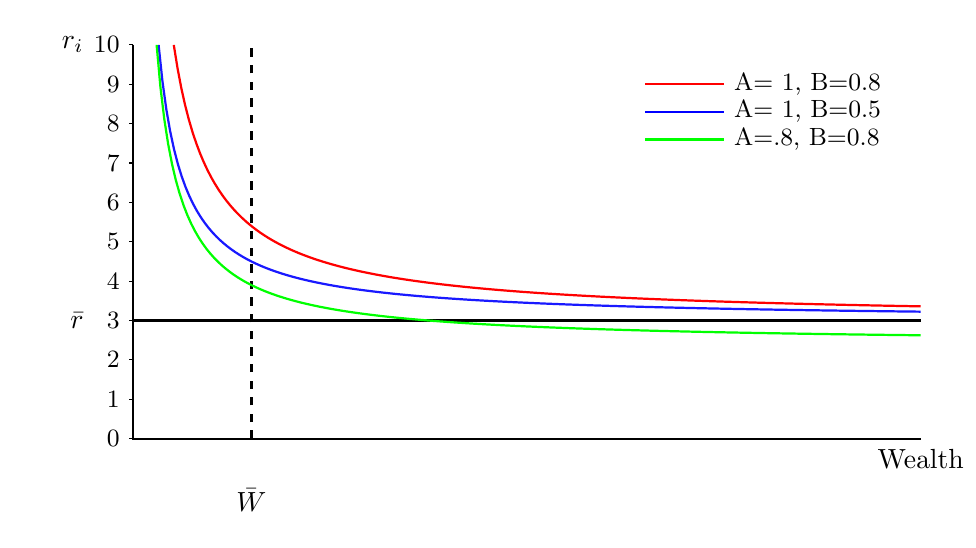
\begin{tikzpicture}[scale=.5]
%\def\bndmax{5}        %https://tex.stackexchange.com/questions/68462/filling-a-complex-region-with-tikz
%\def\bndmin{0.2}
\def \Y {10}  % height of y axis pecent
\def \W {20}  % length  of x axis
\def \Wbar {3} % jmeam wealth
\def \omega {3}
\def \A {1}  %was .5
\def \B {.5}
%Equation   \[ r_i = (A + .5 \frac{\bar{W}}{W_i})\omega\]
\def \Wmin{.63}  %This sets the lower limit fo the 
\def \Wmin{(\B*\Wbar)/(\Y/\omega-\A)} %function to keep in in bounds
	
\tikzset{func/.style={thick,color=blue!90}}	

\draw [thick] (0,\Y)node[left=.5cm]{$r_i$} -- (0,0)--(\W,0)node[below]{Wealth};  	% Axes
\draw [thick] (0,\omega)node[left=.5cm]{$\bar r$} -- (\W,\omega);  	% Axes
\draw [thick,dashed] ( \Wbar,0)node[below=.5cm]{$\bar{W}$} -- (\Wbar,\Y);  	% Axes

\foreach \yi in {0,...,\Y} \draw (0,\yi)--(-.1,\yi)node[left]{\small$\yi$};

\draw[func,domain=\Wmin:\W] plot [samples=200] (\x,{(\A+\B*\Wbar/\x)*\omega});
\def \A {.8}
\draw[func,domain=\Wmin:\W, green] plot [samples=200] (\x,{(\A+\B*\Wbar/\x)*\omega});

\def \A {1}
\def \B {.8}
\draw[func,domain=\Wmin:\W, red] plot [samples=200] (\x,{(\A+\B*\Wbar/\x)*\omega});

\draw [red,  thick](13, 9)--(15,9)node [right, black] {\small A=\ 1,\ B=0.8};
\draw [blue,  thick](13, 8.3)--(15,8.3)node [right, black] {\small A=\ 1,\ B=0.5};
\draw [green, thick](13, 7.6)--(15,7.6)node [right, black] {\small A=.8, B=0.8};
 \end{tikzpicture}
% Figure of cost of borrowing
%\caption{Hypothetical wealth-dependent borrowing cost}
%\label{Fig:BorrowingCost}
%\end{center}
%\end{figure}%

This has a number of immediate implications. First, if agents discount at their borrowing rate, wealthier agents a lower discount rate and therefore value properties more highly. 

Second, given the  common rule that mortgage payments cannot exceed some fraction of disposable income, the wealthy will be able borrow larger amounts and at lower interest rates that the less wealthy. At any distance from the centre they will be able to make a higher bid.
 
If the expected return on a property is greater than the individual cost of borrowing, it would pay any agent to borrow as much as possible and purchase properties as they become available.

\subsubsection{The rate of return on a property purchase $v$}
To explore the implication of the financialization of the urban land market we need a function to calculate the return on a unit of land that reflects the actual gradient of opportunity in financial markets. We begin with the price appreciation, $\Delta P=P_T-P_0 = (1+\dot p)P_0-P_0 $, where $\dot p$ is the rate of price appreciation over the period $T$. Rates will all be specified for the period $T$. Transaction costs, including real estate fees, take a fraction from the value of the final sale.

 The speculator invests a down payment, $D$, and gets back at time $T$ the  increased price $(1+\dot p)P_0$, plus rents, minus any costs and minus the mortgage with interest.
%footnote{We can include a use value, $U$ in place of rent for expatriate owners to represent using the property - say one month a year - when they are not renting the property and a \textbf{vacancy tax},
%$T$ at rate $t$ to affect the speculator's  decision.
 
The rate of return is the value of the gain, $V$,  over the size of the downpayment, $D$, where
\begin{equation}
V =capital\ gain - Interest\ due  	+ Rent  - operating\ cost\    
\end{equation}

The rate of return is $v = \frac{V}{D}$. 

Both the  share of the price  that can be mortgaged, $m$, and the interest rate  and $r$ may be functions of the agent's wealth. $\delta$ represents the net capital gains tax. It makes it possible to capture the capital gains kept. If it is set to one, it simplifies the equations, all is kept. Keeping the variable offers a policy variable to control the return on financial capital.

\begin{eqnarray*}
V  %	&=& capital\ gain - Interest\ due  	+ Rent  - operating\ cost\\
% 	&=& \delta P_T-D \qquad \qquad \quad - (1+\delta r)M \quad	 + R  	-C\\
% 	&=& \delta P _T \qquad-(P_0-M) \quad- (1+\delta r)M 	 + R  	-C\\
%	&=& \delta (1+\dot p)  P_0 -(P_O -M)  -(1+\delta r)mP_0  + R  -C\\
%	&=& \delta (1+\dot p)  P_0 -P_O + M \qquad -(1+\delta r)mP_0  + R -C\\
%	&=&( \delta (1+\dot p)-1)  P_0  + mP_0 \quad -(1+ \delta r)mP_0  + (\rho-\kappa)P_0\\	
%	&=& \left(  \delta (1+\dot p)-1    + m \quad - m(1+\delta r)  + (\rho-\kappa)\right)P_0\\'
%	&=& \left(  \delta (1+\dot p)-1    + m \quad - m-\delta rm  + (\rho-\kappa)\right)P_0\\
&=& \delta(P_T- (1+r)M) \qquad \qquad 	 + R  	-C   - T\\
&=& \delta((1+\dot p)  P_0- (1+r)mP_0)   + \rho P_0  	-\kappa P_0 - tP_0\\
&=&( \delta((1+\dot p)  - (1+r)m) \ + \rho   	-\kappa -t) P_0
\end{eqnarray*}

This is the  net present value of buying, and selling after one period. \textbf{It has  6 exogenous parameters}. Operating revenue and costs $ \rho -\kappa - t$ a present value. 

The rate of return is $v = \frac{V}{D}$. For expat investors, we get a \textbf{decision rule}:\begin{enumerate}
\item  if $v \geq a$ (with some private use?) with no rent,  don't bother renting. 
\item If $v(no\ rent\ and\ tax) < a\leq v(with\ rent)$,  then  rent. 
\item If $ v(with\ rent) \le a $,  then sell 
\end{enumerate}


We can, with some simplifications, write
\begin{eqnarray}
\frac{V}{D}&=&( \delta((1+\dot p)  - (1+r)m) \ + \rho   	-\kappa - t ) \frac{P_0}{D}   \nonumber\\
		&=&( \delta((1+\dot p)  - (1+r)m) \ + \rho   	-\kappa - t ) \frac{P_0}{P_0-mP_0}   \nonumber\\
		&=&\frac{ \delta(1+\dot p  - (1+r)m) \ + \rho   	-\kappa - t } {1-m} \label{Eqn:DecisionRule}
\end{eqnarray}

\subsubsection{Returns on capital are higher for wealthy investors}
\[   r^h=\frac{ \delta(1+\dot p  - (1+r)m) \ + \rho   	-\kappa - t } {1-m}    \]
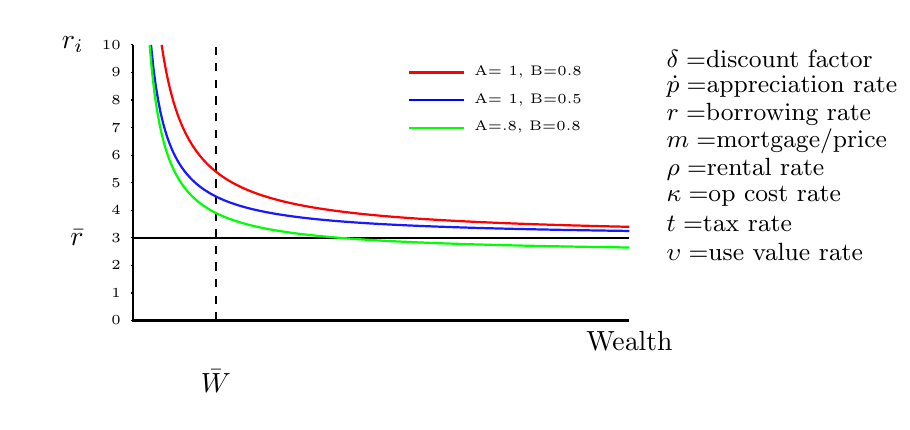
\begin{tikzpicture}[scale=.35]
%\def\bndmax{5}        %https://tex.stackexchange.com/questions/68462/filling-a-complex-region-with-tikz
%\def\bndmin{0.2}
\def \Y {10}  % height of y axis percent
\def \W {18}  % length  of x axis
\def \Wbar {3} % j mean wealth
\def \omega {3}
\def \A {1}  %was .5
\def \B {.5}
%Equation   \[ r_i = (A + .5 \frac{\bar{W}}{W_i})\omega\]
\def \Wmin{.63}  %This sets the lower limit fo the 
\def \Wmin{(\B*\Wbar)/(\Y/\omega-\A)} %function to keep in in bounds
	
\tikzset{func/.style={thick,color=blue!90}}	

\draw [thick] (0,\Y)node[left=.5cm]{$r_i$} -- (0,0)--(\W,0)node[below]{Wealth};  	% Axes
\draw [thick] (0,\omega)node[left=.5cm]{$\bar r$} -- (\W,\omega);  	% Axes
\draw [thick,dashed] ( \Wbar,0)node[below=.5cm]{$\bar{W}$} -- (\Wbar,\Y);  	% Axes

\foreach \yi in {0,...,\Y} \draw (0,\yi)--(-.1,\yi)node[left]{\tiny$\yi$};

\draw[func,domain=\Wmin:\W] plot [samples=200] (\x,{(\A+\B*\Wbar/\x)*\omega});
\def \A {.8}
\draw[func,domain=\Wmin:\W, green] plot [samples=200] (\x,{(\A+\B*\Wbar/\x)*\omega});

\def \A {1}
\def \B {.8}
\draw[func,domain=\Wmin:\W, red] plot [samples=200] (\x,{(\A+\B*\Wbar/\x)*\omega});

\draw [red,  thick](10, 9)--(12,9)node [right, black] {\tiny A=\ 1,\ B=0.8};
\draw [blue,  thick](10, 8)--(12,8)node [right, black] {\tiny A=\ 1,\ B=0.5};
\draw [green, thick](10, 7)--(12,7)node [right, black] {\tiny A=.8, B=0.8};

\def \W {19}  % length  of x axis
\node[right] at (\W,9.5){\small$\delta=$discount factor};
\node[right] at (\W,8.5){\small$\dot p=$appreciation rate};
\node[right] at (\W,7.5){\small$r=$borrowing rate};
\node[right] at (\W,6.5){\small$m=$mortgage/price};
\node[right] at (\W,5.5){\small$\rho=$rental  rate};
\node[right] at (\W,4.5){\small$\kappa=$op cost rate};
\node[right] at (\W,3.5){\small$t=$tax rate};
\node[right] at (\W,2.5){\small$\upsilon=$use value rate};
 \end{tikzpicture}


% 

\chapter{Conclusion}


The economics is clear that this is what's at stake is productivity of cities, the distributive features of the economy and the impact of the middle class.

In a passage that can be seen as a direct precursor to our analysis of urban land rent, Ricardo  wrote in his 1817 Principles of Political Economy, %Early theorists like Ricardo described something can be thought of as describing a three-factor, three-class model with great precision but without the use of mathematics.   

Adding 2 things 1. rent extraction and 2. power law scaling of productivity, we find rent is the breaks on the engine of wealth creation

INTEGRATE- AS THIS SUGGEST ALL GOES TO LANDLOARDS?
What changes over time is the share that goes to each group:

As Ricardo said

\begin{quotation}   
 “The produce of the earth - all that is derived from its surface by the united application of labour, machinery, and capital, is divided among three classes of the community; namely, the proprietor of the land, the owner of the stock or capital necessary for its cultivation, and the labourers by whose industry it is cultivated. ...  But in different stages of society, the proportions of the whole produce of the earth which will be allotted to each of these classes, under the names of rent, profit, and wages, will be essentially different; ”  Chapter 1
\end{quotation}

what's changed is xyz

Ricardo was ``the first writer to take the industrial phenomenon of city life and to create an economy based upon those characteristics.''  \footnote{Simon N. Patten,  The Quarterly Journal of Economics, volume 7, Issue 3, April 1893, Pages 322–352, https://doi.org/10.2307/1884006 }  

Our focus is land rents, but in the context of an urban economy. 

{Ricardo concluded that % , ``It follows then, that 
``the interest of the landlord is always opposed to the interest of every other class in the community.'' }



%Strikingly, Ricardo concluded\footnote{An Essay on the Influence of a low Price of Corn} that, “It follows then, that the interest of the landlord is always opposed to the interest of every other class in the community.” Rents approriated by the land owner are not available to the worker  or the capitalist for re-investment. This is a view that Henry George would later pick up and it is one that we return to in our study, since the issue of urban rents is of great policy importance. 

%----------------------------------------------------------------------
% END MATERIAL
% Bibliography, Appendices, Index, etc.
%----------------------------------------------------------------------

% Bibliography

% The following statement selects the style to use for references.  
% It controls the sort order of the entries in the bibliography and also the formatting for the in-text labels.
\bibliographystyle{plain}
% This specifies the location of the file containing the bibliographic information.  
% It assumes you're using BibTeX to manage your references (if not, why not?).
\cleardoublepage % This is needed if the "book" document class is used, to place the anchor in the correct page, because the bibliography will start on its own page.
% Use \clearpage instead if the document class uses the "oneside" argument
\phantomsection  % With hyperref package, enables hyperlinking from the table of contents to bibliography             
% The following statement causes the title "References" to be used for the bibliography section:
\renewcommand*{\bibname}{References}

% Add the References to the Table of Contents
\addcontentsline{toc}{chapter}{\textbf{References}}

\bibliography{thesis-bib.bib}
% Tip: You can create multiple .bib files to organize your references. 
% Just list them all in the \bibliogaphy command, separated by commas (no spaces).

% The following statement causes the specified references to be added to the bibliography even if they were not cited in the text. 
% The asterisk is a wildcard that causes all entries in the bibliographic database to be included (optional).
% \nocite{*}
%----------------------------------------------------------------------

% Appendices

% The \appendix statement indicates the beginning of the appendices.
\appendix
% Add an un-numbered title page before the appendices and a line in the Table of Contents
\chapter*{APPENDICES}
\addcontentsline{toc}{chapter}{APPENDICES}
% Appendices are just more chapters, with different labeling (letters instead of numbers).
% \chapter[PDF Plots From Matlab]{Matlab Code for Making a PDF Plot}
\label{AppendixA}
% Tip 4: Example (above) of how to get a shorter chapter title for the Table of Contents 
%======================================================================
\section{Using the Graphical User Interface}
Properties of Matab plots can be adjusted from the plot window via a graphical interface. Under the Desktop menu in the Figure window, select the Property Editor. You may also want to check the Plot Browser and Figure Palette for more tools. To adjust properties of the axes, look under the Edit menu and select Axes Properties.

To set the figure size and to save as PDF or other file formats, click the Export Setup button in the figure Property Editor.

\section{From the Command Line} 
All figure properties can also be manipulated from the command line. Here's an example: 
\begin{verbatim}
x=[0:0.1:pi];
hold on % Plot multiple traces on one figure
plot(x,sin(x))
plot(x,cos(x),'--r')
plot(x,tan(x),'.-g')
title('Some Trig Functions Over 0 to \pi') % Note LaTeX markup!
legend('{\it sin}(x)','{\it cos}(x)','{\it tan}(x)')
hold off
set(gca,'Ylim',[-3 3]) % Adjust Y limits of "current axes"
set(gcf,'Units','inches') % Set figure size units of "current figure"
set(gcf,'Position',[0,0,6,4]) % Set figure width (6 in.) and height (4 in.)
cd n:\thesis\plots % Select where to save
print -dpdf plot.pdf % Save as PDF
\end{verbatim}

% GLOSSARIES (Lists of definitions, abbreviations, symbols, etc. provided by the glossaries-extra package)
% -----------------------------
\printglossary
\cleardoublepage
\phantomsection		% allows hyperref to link to the correct page

%----------------------------------------------------------------------
\end{document} % end of logical document
